
% options:
% thesis=B bachelor's thesis
% thesis=M master's thesis
% czech thesis in Czech language
% english thesis in English language
% hidelinks remove colour boxes around hyperlinks
\documentclass[thesis=B,english]{FITthesis}[2012/10/20]



% ******************************************************************
% *************************   PACKAGES   ***************************
% ******************************************************************

\usepackage{todonotes} % causing Marginpar on page x moved
\usepackage{xcolor}

\newcommand\TODO[1]{\textcolor{red}{#1}}


% \usepackage[utf8]{inputenc} % LaTeX source encoded as UTF-8
% \usepackage[latin2]{inputenc} % LaTeX source encoded as ISO-8859-2
% \usepackage[cp1250]{inputenc} % LaTeX source encoded as Windows-1250

\usepackage{graphicx} %graphics files inclusion
% \usepackage{subfig} %subfigures
% \usepackage{amsmath} %advanced maths
% \usepackage{amssymb} %additional math symbols

\usepackage{pgfplots}
\pgfplotsset{compat=1.10}
\usetikzlibrary{calc}

\usepackage{adjustbox}



\usepackage[detect-none]{siunitx}


%\usepackage{tikz}

\usepackage{dirtree} %directory tree visualization

% other packages
\usepackage{enumerate}

% Mathematic Packages
% mathbb - double -> R,N,Z ...
% mathcal - curved -> N, O
% sigma tilde hat 
\usepackage{amsmath}
\usepackage{amssymb}
\usepackage{amsthm}
\usepackage{mathrsfs}

% \begin{description}
% 	\item[BP] 
% 	\item[DP] 
% \end{description}

% h float specifier changed to ht -- image floating environment error


% \begin{itemize}
% 	\item 
% 	\item 
% \end{itemize}


% - (known as an hyphen) between the elements of compound words
% -- (known as an en-dash) for ranges "3–7"
% --- (known as a em-dash) punctuation for digressions in a sentence—though how it differs from a parenthetical comment I have never known—which is why you don't see it much


% downloaded - in root folder
\usepackage{kbordermatrix}% http://www.hss.caltech.edu/~kcb/TeX/kbordermatrix.sty


% **** PSEUDOCODE ****
\usepackage{amsfonts}
\usepackage[titlenumbered, ruled, linesnumbered]{algorithm2e}

% ***& MY MACROS ****
% mymacros.sty
% file with my macros
\usepackage{mymacros}

% % list of acronyms
% \usepackage[acronym,nonumberlist,toc,numberedsection=autolabel]{glossaries}
% \iflanguage{czech}{\renewcommand*{\acronymname}{Seznam pou{\v z}it{\' y}ch zkratek}}{}
% \makeglossaries


% \usepackage[style=numeric]{biblatex}
% \addbibresource{BP_ja_bibliography.bib}
% ...
% \printbibliography

% ******************************************************************
% **************************   HEADER   ****************************
% ******************************************************************

\department{Department of Applied Mathematics}
\title{Probabilistic algorithms for computing the LTS estimate}
\authorGN{Martin} %author's given name/names
\authorFN{Jen{\v c}} %author's surname
\author{Martin Jen{\v c}} %author's name without academic degrees
\authorWithDegrees{Martin Jen{\v c}} %author's name with academic degrees
\supervisor{Ing. Karel Klouda, Ph.D.}
\acknowledgements{I wish to express my sincere thanks to Ing. Karel Klouda, Ph.D., chair of the Department of Applied Mathematics, for providing me with all the facilities and encouragement necessary in finishing this work.}

\abstractEN{The least trimmed squares method is a robust version of the method of least squares which is an essential tool of regression analysis used to find an estimate of coefficients in the linear regression model. Computing the least trimmed squared estimate is known to be NP-hard, hence only suboptimal probabilistic algorithms are usually used in practice. Besides describing those algorithms, we propose a few ways of combining those algorithms to obtain better performance.}

%%


\abstractCS{Metoda nejmen{\v s}{\'i}ch usekan{\'y}ch {\v c}tverc{\r u} je robustn{\'i} verz{\'i} zn{\'a}m{\'e} metody nejmen{\v s}{\'i}ch {\v c}tverc{\r u}, jedn{\'e} ze z{\'a}kladn{\'i}ch metod regresn{\'i} anal{\'y}zy, pou{\v z}{\'i}van{\'e} k odhadov{\'a}n{\'i} koeficient{\r u} line{\'a}rn{\'i}ho regresn{\'i}ho modelu. V{\'y}po{\v c}et odhadu pomoc{\'i} metody nejmen{\v s}{\'i}ch usekan{\'y}ch {\v c}tverc{\r u} je zn{\'a}m jako NP-t{\v e}{\v z}k{\'y} a proto jsou v praxi nej{\v c}ast{\v e}ji pou{\v z}{\'i}v{\'a}ny pouze subotim{\'a}ln{\'i} pravd{\v e}podobnostn{\'i} algoritmy. Mimo popisu t{\v e}chto algoritm{\r u} navrhneme n{\v e}kolik zp{\r u}sob{\r u} jak je zkobinovat za {\'u}{\v c}elem dosa{\v z}en{\'i} lep{\v s}{\'i}ch v{\'y}sledk{\r u}.}
\placeForDeclarationOfAuthenticity{Prague}
\keywordsCS{nejmen{\v s}{\'i} usekan{\'e} {\v c}tverce, LTS odhad, linearn{\'i} regrese, robustn{\'i} statistika, nejmen{\v s}{\'i} {\v c}tverce, chybn{\'a} pozorovan{\'i}}
\keywordsEN{least trimmed squares, LTS estimate, linear regression, robust statistics, ordinary least squares, outliers}
\declarationOfAuthenticityOption{1} %select according to the desired license (integer 1-6)
% \website{http://site.example/thesis} %optional thesis URL



% ******************************************************************
% ***********************   MAIN DOCUMENT   ************************
% ******************************************************************

% CONTENTS SUB SECTION
\setcounter{tocdepth}{3}
\setcounter{secnumdepth}{3}
%%

\begin{document}
% \newacronym{CVUT}{{\v C}VUT}{{\v C}esk{\' e} vysok{\' e} u{\v c}en{\' i} technick{\' e} v Praze}
% \newacronym{FIT}{FIT}{Fakulta informa{\v c}n{\' i}ch technologi{\' i}}



% ******************************************************************
% **************************  CHAPTERS  ****************************
% ******************************************************************

\setsecnumdepth{part}
\chapter{Introduction}
Goal of this thesis is to research currently used algorithms for calculation Least trimmed squares. Least trimmed squares was first introduced in 1984 and since that time couple of researchers came up couple of solutions. Beside that we'll propose extension of current algorithms which was never used before. We'll show that this updated algorithm is fast enough and also gives same or better results than currently used algorithms. We'll also compare speed  and performance of this algorithms on various data sets both from literature and also using our custom data generator which provides very flexible way of generating data with outliers. 
We'll extend all those algorithms and implement all of them both in C++ an python. 
We'll implement python library with C++ bac end which will provide all of the currently used algorithms.

In first chapter we'll introduce linear regression and ordinary least squares method and it's downfalls. We'll introduce robust statistic and methods of evaluating robust models.
In second chapters we'll analyze all of the algorithms together with is time complexity etc

%% psat v pritomnem case; ale muzeme psat v kapitole se budeme zabyvat % ale i kapitola 5 se zabyva

\subsection{Conclusion}
There is still lot of future works on least trimmed squares. Proof of couple of thoughts is still about to come. 

% je lepsi citovat od "zdroje" tedy k clanku kde to bylo prvne zadefinovane



\setsecnumdepth{all}
% \listoftodos

\chapter{Least trimmed squares}
In this chapter, we introduce one of the most common regression analysis models which is known as the linear regression model. It aims to model the relationship between one variable which is called \defterm{dependent} and one or more variables which are called \defterm{explanatory}. The relationship is based on a model function with parameters which are not known in advance and are to be estimated from data. We also describe one of the most common methods for finding those parameters in this model, namely the ordinary least squares method. It is important to note that all vectors in this text are considered as column vectors. On the other hand, we denote a row vector as a transposed vector.



%%%%%%%%%%%%%%%%%%%%%%%%%%%%%%%%%%%%%%%%%%%%%%%%%%%%%%%%%%%%%%%%%%%%%%%%%%%%%%%%%%%%%%%%%%%%%%%%%%%%
%%%%%%%%%%%%%%%      SECTION: LINEAR REGRESSION MODEL     %%%%%%%%%%%%%%%%%%%%%%%%%%%%%%%%%%%%%%%%%%
%%%%%%%%%%%%%%%%%%%%%%%%%%%%%%%%%%%%%%%%%%%%%%%%%%%%%%%%%%%%%%%%%%%%%%%%%%%%%%%%%%%%%%%%%%%%%%%%%%%%

\section{Linear regression model}
\begin{definition}\label{definition:lr_model}
    The \defterm{linear regression model} is given by
\begin{equation}
        y = \vec{x}^T\vec{w} + \varepsilon ,
\end{equation}
where $y \in \mathbb{R}$ is a random variable which is called \defterm{dependent variable} and $\vec{x}^T = (x_1, x_2, \ldots, x_p)$ is a vector of \defterm{explanatory variables}. Usually we call $x_i$ a regressor. Finally $\varepsilon \in \mathbb{R}$ is a random variable called \defterm{noise} or \defterm{error}. The vector $\vec{w} = (w_1, w_2, \ldots, w_p)$ is a vector of parameters called  \defterm{regression coefficients}. 
\end{definition}
In regression analysis we aim to estimate the $\vec{w}$ using $n$ measurements of $y$ and $\vec{x}$. We can write this in matrix form 

% In practice, we usually deal with multiple dependent variables so we define multiple linear regression model.

% \begin{definition}\label{definition:lr_model_multiple}
% The \defterm{multiple linear regression model} is 
% \begin{equation}
%         y_i = \vec{x_i}^T\vec{w} + \varepsilon_i,\\ i=1,\ldots , n.
% \end{equation}
% It is common to write the whole model in a matrix form

\begin{equation}
    \vec{y} = \vec{X}\vec{w} + \vec{\varepsilon}    \numberthis
\end{equation} where

\[ 
\vec{y} = \begin{bmatrix}
    y_{1} \\
    y_{2} \\
    \vdots \\
    y_{n}
  \end{bmatrix}\\,
 \vec{X} = \begin{bmatrix}
    \vec{x_1}^T \\
    \vec{x_2}^T \\
    \vdots \\
    \vec{x_n}^T
\end{bmatrix}
=
\begin{bmatrix}
    x_{11} & x_{12} & x_{13} & \dots  & x_{1p} \\
    x_{21} & x_{22} & x_{23} & \dots  & x_{2p} \\
    \vdots & \vdots & \vdots & \ddots & \vdots \\
    x_{n1} & x_{n2} & x_{n3} & \dots  & x_{np}
\end{bmatrix}\\,
\vec{w} = \begin{bmatrix}
    w_{1} \\
    w_{2} \\
    \vdots \\
    w_{p}
  \end{bmatrix}\\,
  \vec{\varepsilon} = \begin{bmatrix}
    \varepsilon_{1} \\
    \varepsilon_{2} \\
    \vdots \\
    \varepsilon_{n}
  \end{bmatrix}
\]
This means that we can think of rows of matrix $\vec{X}$ as columns vectors $\vec{x_i}$ written into the row.

It is assumed that errors are independent and identically distributed so that $\vec{\varepsilon} \sim \mathcal{N}(0,\,\sigma^{2})$.
% \end{definition}
%It this work we talk about the multiple linear regression model, but for simplicity, we call it merely the linear regression model.

\begin{note}
    It is usual refer to given $\vec{X}$ and $\vec{y}$ as to \defterm{data set} and to $y_i$ with corresponding $\vec{x_i}$ as to $i$th \defterm{data sample} or \defterm{observation}.
\end{note}

%%%% OK TO HERE
\subsection{Prediction with the linear regression model}
The linear regression model contains the vector $\vec{w}$ of regression coefficients which are unknown and which we need to estimate in order to be able to use the model for predictions. Let us assume that we already have estimated regression coefficients as $\vec{\hat{w}}$. Then the predicted values of $y$ are given by
\begin{equation}
    \hat{y} = \vec{\hat{w}}^T\vec{x}. \numberthis
\end{equation}
The true value of $y$ is given by 
\begin{equation}
    y = \vec{w^{*}}^T\vec{x} + \varepsilon
\end{equation}
where $ \vec{w^{*}}$  represents actual regression coefficients which we aim to estimate. 

Because we assume linear dependence between dependent variable $y$ and explanatory variables $\vec{x}$ which we assume to be non-random, then what makes $y$ random variable is a random variable $\varepsilon$. Because we assume that $\mathbb{E}(\varepsilon) = 0$ we can see that 

\begin{equation} \label{equation:vary}
\mathbb{E}(y) = \vec{x}^T\vec{w} + \mathbb{E}(\varepsilon) = \vec{x}^T\vec{w}
\end{equation}
so $\hat{y}$ is a point estimation of the expected value of $y$.

\subsubsection*{Intercept}
In real world situations it is not usual that $\mathbb{E}(\varepsilon) = 0$. Consider this trivial example.
\begin{example} \label{example:intercept}
Let us consider that $y$ represents price of the room and $x$ represents the number of the windows in such a room. If this room does not have windows thus $x = 0$ and $\mathbb{E}(\varepsilon) = 0$ then $ y = wx + \varepsilon$ equals zero. But it is very unlikely that room without windows is free. 
\end{example}

Because of that, it is very common to include one constant regressor $x_1 = 1$. The corresponding coefficient $w_1$ of $\vec{w}$ is called an \defterm{intercept}. We refer this model as a \defterm{model with an intercept}. The intercept then corresponds to expected value of $y$ when all regressors are zero and prevent the problem from Example~\ref{example:intercept}. This means that intercept can be assumed as a shift so that it corresponds to $\mathbb{E}(\varepsilon) = \mu$. With regards to this fact we can still assume that in the model with intercept $\varepsilon \sim \mathcal{N}(0,\,\sigma^{2})$.
In this work, we consider the model with the intercept. This means that we consider $\vec{x} = (x_1, x_2 \ldots x_p)$ where constant $x_1 = 1$ represents intercept.  
\begin{note}
Sometimes in the model with an intercept, the explanatory variable $\vec{x}$  is marked as $\vec{x} \in \mathbb{R}^{p+1}, \vec{x} = (x_0, x_1 \ldots x_p)$, 
which means that actual observation $\vec{x} \in \mathbb{R}^p$ and the intercept $x_0 = 1$ is explicitly marked.
\end{note} 


%%%%%%%%%%%%%%%%%%%%%%%%%%%%%%%%%%%%%%%%%%%%%%%%%%%%%%%%%%%%%%%%%%%%%%%%%%%%%%%%%%%%%%%%%%%%%%%%%%%%
%%%%%%%%%%%%%%%      SECTION: ORDINARY LEAST SQUARES    %%%%%%%%%%%%%%%%%%%%%%%%%%%%%%%%%%%%%%%%%%%%
%%%%%%%%%%%%%%%%%%%%%%%%%%%%%%%%%%%%%%%%%%%%%%%%%%%%%%%%%%%%%%%%%%%%%%%%%%%%%%%%%%%%%%%%%%%%%%%%%%%%

\section{Ordinary least squares}
We want to estimate $\vec{w}$ so that an error of the model on the whole data set is the least possible. This error is measured by a \defterm{loss function} 
$L : \mathbb{R}^2 \rightarrow  \mathbb{R}$,
which in case of the \defterm{ordinary least squares} (OLS) method is quadratic loss function $L(y, \hat{y}) := (y - \hat{y})^2$. 
So the idea is to find $\vec{\hat{w}}$ so that it minimizes the sum of squared \defterm{residuals}
\begin{equation}
    r_i(\vec{w}) =y_i - \hat{y_i} = y_i - \vec{x_i}^T\vec{w} ,\ i = 1,2,\ldots ,n.
\end{equation}
This is commonly know as residual sum of squares $RSS$
\begin{equation}
    RSS(\vec{w}) = \sum\limits_{i=1}^n r_i^2(\vec{w}) = \sum\limits_{i=1}^n (y_i - \vec{w}^T\vec{x_i})^2.
\end{equation}
\begin{definition} The RSS as the function of $\vec{w}$ is an \defterm{objective function} for OLS
    \begin{equation}
        \of^{(OLS,\vec{X}, \vec{y})}(\vec{w}) = \sum\limits_{i=1}^n (y_i - \vec{w}^T\vec{x_i})^2 = (\vec{Y} - \vec{X}\vec{w})^T(\vec{Y} - \vec{X}\vec{w}).
    \end{equation}
\end{definition}
The point of the minimum of this function 
\begin{equation}
\vec{\hat{w}^{(OLS, n)}}  = \argmin_{\vec{w} \in \mathbb{R}^p} \of^{(OLS,\vec{X}, \vec{y})}(\vec{w})
\end{equation}
is a the ordinary least squares estimate of regression coefficients.

To find the minimum of this function, we first need to find the gradient by calculating all partial derivatives
\begin{equation}
    \frac{\partial {\of^{(OLS,\vec{X}, \vec{y})}} }{\partial w_j} = \sum\limits_{i=1}^n 2(y_i - \vec{w}^T\vec{x_i})(-x_{ij}) \\, \ \ j \in \{{1,2,\ldots,p\}}. 
\end{equation}
By this we obtain the gradient 
\begin{equation}
    \nabla \of^{(OLS,\vec{X}, \vec{y})} = -\sum\limits_{i=1}^n 2(y_i - \vec{w}^T\vec{x_i})\vec{x_i}. 
\end{equation}
Putting gradient equal to zero we get the so called \defterm{normal equations}
\begin{equation}
    -\sum\limits_{i=1}^n 2(y_i - \vec{w}^T\vec{x_i})\vec{x_i} = 0 
\end{equation}
that can be rewritten in a matrix form as 
\begin{equation}    \label{equation:zerogradient}
    \vec{X}^T\vec{y} - \vec{X}^T\vec{X}\vec{w} = 0.
\end{equation}

Let us now construct the hessian matrix using second-order partial derivatives:
\begin{equation}
    \frac{\partial^2{\of^{(OLS,\vec{X}, \vec{y})}} }{\partial w_h\partial w_j} = \sum\limits_{i=1}^n 2(- x_{ik})(-x_{ij}) \\, \ \ h \in \{{1,2,\ldots,p\}}. 
\end{equation}
We get 
\begin{equation}
    \vec{H_{\of^{(OLS,\vec{X}, \vec{y})}}} = 2\vec{X}^T\vec{X}.
\end{equation}

We can see that hessian $\vec{H_{\of^{(OLS,\vec{X}, \vec{y})}}}$ is always positive semi-definite because for all $\vec{s} \in \mathbb{R}^p$

\begin{equation}
    \vec{s}^T(2\vec{X}^T\vec{X})\vec{s} = 2(\vec{X}\vec{s})^T(\vec{X}\vec{s}) =  2 \norm{\vec{X}\vec{s}}^2
\end{equation}

It is easy to prove that twice differentiable function is convex if and only if the hessian of such function is positive semi-definite. Moreover, any local minimum of the convex function is also the global one. Hence the solution of~\eqref{equation:zerogradient} gives us the global minimum. 

Assuming that $\vec{X}^T\vec{X}$ is a regular matrix, its inverse exists, and the solution can be explicitly written as

\begin{equation} \label{wols}
    \vec{\hat{w}}^{(OLS,n)} = (\vec{X}^T\vec{X})^{-1}\vec{X}^T\vec{y}, 
\end{equation}
where $(OLS,n)$ denotes that $\vec{\hat{w}}^{(OLS,n)}$ is the estimate of true regression coefficients given by the OLS method for $n$ observations. 

Moreover, we can see that if $\vec{X}^T\vec{X}$ is a regular matrix, then the hessian $\vec{H_{\of^{(OLS,\vec{X}, \vec{y})}}}$ is positive definite and $\of^{(OLS,\vec{X}, \vec{y})}$ is strictly convex and $\vec{\hat{w}}^{(OLS,n)}$ is the unique strict global minimum.

% norms can be used to create distance as d(x,y) = || x - y ||
% but not all distances have corresponding norm! trivial example. d(x,x) = 0, d(x,y) = 1

\subsection{Properties of the OLS estimate}
Gauss-Markov theorem~\cite{mccullagh2018generalized} tells us that if particular assumptions about the regression model are fulfilled then the OLS estimate is unbiased and efficient. Gauss-Markov theorem states that OLS is the best linear unbiased estimator (BLUE). Being an efficient estimate means that any other linear unbiased estimate has the same or higher variance. The most important conditions are:

\begin{itemize} \label{ols:assumptions}
  \item Expected value of errors is zero.
  \item Errors are independently distributed and uncorrelated thus \\ $cov(\varepsilon_i, \varepsilon_j), \ i, j = 1, 2 \ldots , n, \ \ i \neq j$
 % \item Regressors $\vec{x_i}, i = 1, 2, \ldots , n$ and corresponding errors 
%$\varepsilon_i, \ i = 1,2, \ldots , n$ are uncorrelated.
 \item All errors have same finite variance. This is known as \defterm{homoscedasticity}.
\end{itemize}

% \begin{note}
%  As described in Example~\ref{example:intercept} the first assumption is usually fulfilled if we use the model with intercept. Rest of the conditions, on the other hand, are rarely met.
% \end{note}

There are also other theorems which describe properties of OLS under specific conditions, but they are out if the scope of this work.


%%%%%%%%%%%%%%%%%%%%%%%%%%%%%%%%%%%%%%%%%%%%%%%%%%%%%%%%%%%%%%%%%%%%%%%%%%%%%%%%%%%%%%%%%%%%%%%%%%%%
%%%%%%%%%%%%%%%      SECTION: ROBUST STATISTICS      %%%%%%%%%%%%%%%%%%%%%%%%%%%%%%%%%%%%%%%%%%%%%%%
%%%%%%%%%%%%%%%%%%%%%%%%%%%%%%%%%%%%%%%%%%%%%%%%%%%%%%%%%%%%%%%%%%%%%%%%%%%%%%%%%%%%%%%%%%%%%%%%%%%%

\section{Robust statistics} \label{section:roboust}
Standard statistics methods rely on multiple assumptions and fail if those assumptions are not met. The goal of the robust statistics is to produce acceptable results even when the data are from some unconventional distributions or if data contains outliers or errors which are not normally distributed. 

Such assumptions about the OLS method are described in Section~\ref{ols:assumptions}. Before we explain what happens if those conditions are not met or met only partially let us describe one of the most common reasons why assumptions are false.

\subsection{Outliers}
We stated many assumptions that are required for the OLS method to produce a acceptable estimate of $\vec{\hat{w}}$. Unfortunately, in real conditions, these assumptions are often false so that the ordinary least squares do not guarantee to return reasonable results. One of the most common reasons for the assumptions being not met are observations called outliers.

Outliers are for instance erroneous measurements such as transmission errors or noise. Another common reason for outliers is that nowadays the data are automatically processed by computers. Sometimes we are also given data which are heterogeneous in the sense that they contain data from multiple regression models. In some sense outliers are inevitable. One would say that we should be able to eliminate them by precise examination, repair or removal of such data. That is possible in some cases, but often the data we are dealing with are too big and highly dimensional to check.

The robust methods are sometimes not only useful to create models that are not being unduly affected by the presence of outliers but also capable of identifying data which seems to be outliers. 

We use terminology from~\cite{rouss:1990} to describe certain types of outliers. Let us have observation $(y_i, \vec{x_i})$. If the observation is not outlying in any direction we call it \defterm{regular observation} . If it is outlying in direction of the explanatory variable $\vec{x_i}$  we call it \defterm{leverage point}. We have two types of leverage points. If $\vec{x_i}$ is outlying but $(y_i, \vec{x_i})$ follows the liner pattern we call it a \defterm{good leverage point}. If it does not follow such a pattern we call it \defterm{bad leverage point}. Finally if $(y_i, \vec{x_i})$ is  outlying only in direction of $y_i$, we call it a \defterm{vertical outlier}.

\subsection{Measuring robustness}
There are a couple of tools to measure the robustness of an estimate. One of the most popular one is called \defterm{breakdown point}. Others are \defterm{empirical influence function} and \defterm{influence function and sensitivity curve}.  Here we describe only breakdown point right now. More on robustness measures can be found in~\cite{hampel1986robust}.

\begin{definition}
    Let $T$ be a statistics, $\vec{x} = (x_1, x_2,\ldots,x_n)$ be an $n$-element random sample and $T_n(\vec{x})$ value of this statistics. The breakdown point of $T$ at sample $\vec{x}$ is defined using sample $\vec{\overline{x}}^{(k)}$, that arose by replacing $k$ points from the original sample $\vec{x}$ with random values $x_i$. Then the \defterm{breakdown point} is 

\begin{equation}
    \bdpoint(T,\vec{x_n} ) = \frac{1}{n} \min S_{T, \vec{x_n}} , 
\end{equation}
where 
\begin{equation}
   S_{T, \vec{x_n}, D} = 
  \left\{ k \in \{{1,2, \ldots ,n\}} : \sup_{ \vec{\overline{x}}^{(k)} } \norm{T_n(\vec{x}) - T_n(\vec{\overline{x}}^{(k)})} = \infty   \right\}.  
\end{equation}
\end{definition}

This definition is says that the breakdown point is the function of the minimal number of observations needed to be changed so that the estimator gives arbitrarily biased results.

Intuitively, a reasonable breakdown point should not be higher than~$0.5$~\cite{rouss:1986} ; if more than $50\%$ of the data is exchanged, the model of exchanged data should override the model of the original data. 

In the case of the OLS estimator, one outlier is enough to increase the value of $\vec{\hat{w}}^{(OLS,n)}$ to any desired value~\cite{agullo2001new} thus 
\begin{equation}
    \bdpoint(\vec{\hat{w}}^{(OLS,n)},\vec{x_n} ) = \frac{1}{n}.
\end{equation}

\begin{figure}[h]
    \centering
    % \missingfigure{Image visualizing  one C-step}
    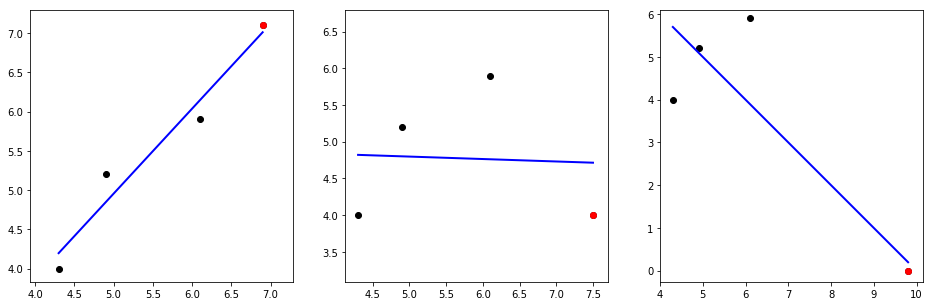
\includegraphics[width=12cm]{img/outlier_regression}
    \caption{Change of the regression hyperplane when one of the four observations (highlighted with red color) starts to deviate from the linear pattern.}
    \label{figure:outlier:hyperplane}
\end{figure}

Figure~\ref{figure:outlier:hyperplane} gives us an idea of how one outlier may change the hyperplane given by the OLS estimator of regression coefficients.



    

For an increasing number of the data samples $n$ the breakdown point of $\vec{\hat{w}}^{(OLS,n)}$ tends to zero. We can see that ordinary least squares estimator is not resistant to outliers at all. Due to this fact, multiple robust estimators alternatives to the OLS have been proposed.




%%%%%%%%%%%%%%%%%%%%%%%%%%%%%%%%%%%%%%%%%%%%%%%%%%%%%%%%%%%%%%%%%%%%%%%%%%%%%%%%%%%%%%%%%%%%%%%%%%%%
%%%%%%%%%%%%%%%      SECTION: LEAST TRIMMED SQUARES       %%%%%%%%%%%%%%%%%%%%%%%%%%%%%%%%%%%%%%%%%%
%%%%%%%%%%%%%%%%%%%%%%%%%%%%%%%%%%%%%%%%%%%%%%%%%%%%%%%%%%%%%%%%%%%%%%%%%%%%%%%%%%%%%%%%%%%%%%%%%%%%
\section{Least trimmed squares}
The least trimmed squares (LTS) estimator is a robust version of the OLS estimator. In this section, we give a definition and show that its breakdown point is variable and can go up to the maximum possible value of breakdown point, thus~$0.5$.

\begin{definition} \label{definition:of:lts:real}
Let us have $\vec{X} \in \mathbb{R}^{n,p}$, $\vec{y} \in \mathbb{R}^{n,1}$, 
    $\vec{w} \in \mathbb{R}^p$ and $h$, $ n/2 \leq h \leq n$. The objective function of LTS for data $\vec{X}$ and $\vec{y}$ is
    \begin{equation}  
        \of^{(LTS,h, n)}(\vec{w}) =  \sum\limits_{i=1}^h r_{i:n}^2(\vec{w})  
    \end{equation}
\end{definition}
where $r_{i:n}^2(\vec{w})$ denotes the $i$th smallest squared residuum at $\vec{w}$, i.e. 
\begin{equation}
    r_{1:n}^2(\vec{w}) \leq r_{2:n}^2(\vec{w}) \leq \ldots \leq r_{n:n}^2(\vec{w}).   
\end{equation} 

Even though that objective function of LTS seems similar to the OLS objective function, finding the minimum is far more complex because the order of the least squared residuals depends on $\vec{w}$. Moreover, $r_{i:n}^2(\vec{w})$ residuum is not uniquely determined if more squared residuals have same value. This makes finding the LTS estimate non-convex optimization problem and, in fact, finding the global minimum is NP-hard~\cite{bernholt2006robust}. 

\subsection{Discrete objective function} \label{sectionofltsdiscrete}
The LTS objective function from Definition~\ref{definition:of:lts:real} is not differentiable and not convex, so we are unable to use the same approach as with the OLS objective function. Let us transform this objective function to a discrete version which is easier to use by algorithms to minimize it.

Let us assume for now that we know the vector $\vec{\hat{w}^{(LTS, h, n)}}$ of estimated regression coefficients minimizing the LTS objective function. Let $\pi$ be the permutation of $\hat{n} = \{{1,2,\ldots, n\}}$ such that 

\begin{equation}
    r_{i:n}(\vec{\hat{w}^{(LTS, h, n)}}) = r_{\pi(j)}(\vec{\hat{w}^{(LTS, h, n)}})\\, \ \ j \in \hat{n}.
\end{equation}
Put
 \begin{equation}
   Q^{(n,h)} = \left\{ \vec{m} \in \mathbb{R}^n \ | \ m_i \in \{{0, 1\}} \\,i \in \hat{n} \\,   \sum\limits_{i=1}^n  m_i = h \right\},
\end{equation}
which is simply the set of all vectors $\vec{m} \in \mathbb{R}^n$ which contain $h$ ones and $n-h$ zeros. Let $\vec{m}^{(LTS)} \in Q^{(n,h)}$  such that  $m^{(LTS)}_j = 1$ when $\pi(j) \leq h$ and $m^{(LTS)}_j = 0$ otherwise. Then

\begin{equation} \label{ltshat}
    \vec{\hat{w}^{(LTS, h, n)}} =  
  \argmin_{\vec{w} \in \mathbb{R}^p} \sum\limits_{i=1}^h r_{i:n}^2(\vec{w}) = 
  \argmin_{\vec{w} \in \mathbb{R}^p} \sum\limits_{i=1}^n m^{(LTS)}_i r_{i}^2(\vec{w}). 
\end{equation}
This means that if we know the vector $\vec{m}_{LTS}$ than we can compute the LTS estimate as the OLS estimate with $\vec{X}$ and $\vec{Y}$ multiplied by the diagonal matrix $\vec{M}_{LTS} = diag(\vec{m}^{(LTS)})$:

\begin{equation}  \label{lts:discrete:objective}
    \vec{\hat{w}^{(LTS, h, n)}} = (\vec{X}^T\vec{M}_{LTS}\vec{X})^{-1}\vec{X}^T\vec{M}_{LTS}\vec{y}.
\end{equation}
In other words, finding the minimum of the LTS objective function can be done by finding the OLS estimates~\eqref{lts:discrete:objective} for all vectors 
$\vec{m} \in Q^{(n,h)}$. 
Thus if we denote $\vec{X_{M}} = \vec{M}\vec{X} $ and $\vec{y_{M}} = \vec{M}\vec{y}$ which corresponds to the $h$-element subsets of $\vec{X}$ and $\vec{Y}$, then as described in~\cite{kloudaVyzkumnyUkol},


% \of^{(LTS,\vec{X_{M}}, \vec{y_{M}} }(\vec{m})


\begin{align} \label{kloudaodvozeni}
\minim_{\vec{w} \in \mathbb{R}^p} 
    \of^{(LTS, h, n)}(\vec{w})  
&=\minim_{\vec{w} \in \mathbb{R}^p} 
    \sum\limits_{i=1}^h r_{i:n}^2(\vec{w})  \\
&= \minim_{\vec{w} \in \mathbb{R}^p,\vec{m} \in Q^{(n,h)}} 
        \sum\limits_{i=1}^n m_i r_{i}^2(\vec{w})\\
&= \minim_{\vec{m} \in Q^{(n,h)}} 
            \Big( \minim_{\vec{w} \in\mathbb{R}^p} 
            \of^{(OLS,\vec{M}\vec{X},  \vec{M}\vec{y} )} (\vec{w}) \Big)\\
&= \minim_{\vec{m} \in Q^{(n,h)}} 
            \Big(\minim_{\vec{w} \in\mathbb{R}^p}  
            \norm{ \vec{M}\vec{y} -   \vec{M}\vec{X}\vec{w}  }^2 \Big).
\end{align}

Substituting $\vec{w}$ with the OLS estimate as in~\eqref{ltshat} we get
%% TODO %%%%%%%%%%%%%%%%%%%%%%%%%%%%%%
\begin{align*}
\vec{\hat{w}^{(LTS, h, n)}}
&=  \minim_{\vec{m} \in Q^{(n,h)}} 
    \Big( \norm{ \vec{M}\vec{y} -  \vec{M}\vec{X}(\vec{X}^T\vec{M}\vec{X})^{-1}\vec{X}^T\vec{M}\vec{y}  }^2 \Big)
\end{align*}

We get the discrete objective function with domain $\vec{m} \in Q^{(n,h)}$

\begin{equation} \label{oflts_discrete}
    \oflts(\vec{m}) =  \norm{ \vec{M}\vec{y} -  \vec{M}\vec{X}(\vec{X}^T\vec{M}\vec{X})^{-1}\vec{X}^T\vec{M}\vec{y}  }^2.
\end{equation}

Minimizing this OF could by done straightforwardly by iterating over the $Q^{(n,h)}$ set. Unfortunately, this set has cardinality equal to $\binom{n}{h}$, which is huge, so this approach is infeasible for bigger data sets. Multiple algorithms were proposed to overcome this problem. Majority of them are probabilistic algorithms, but besides those, some exact algorithms were proposed. 

Finally, let us point out some fact about the number $h$ of non-trimmed residuals and how it makes least trimmed squares robust.
The LTS reaches maximum breakdown point $0.5$ at $h = [(n/2] + [(p+1)/2]$~\cite{agullo2001new}.
This means that up to $50\%$ of the data can be outliers. In practice, the portion of outliers is usually lower; if an upper bound on the percentage of outliers is known,  $h$ should be set to match this percentage.
\chapter{Algorithms}

% mathbb - double -> R,N,Z ...
% mathcal - curved -> N, O
% sigma tilde hat 
In previous chapter we've covered necessary theory needed to implement algorithms that are in this chapter. Let's quickly recap most important fact that we know so far.

With robust linear regression problem we assume that our model with intercept
\begin{equation}
		y_i = \vec{w}^T\vec{x_i} + \varepsilon_i
\end{equation}
where $\varepsilon_i \sim \mathcal{N}(0, \sigma^2)$ is $i.i.d.$ random variable has some displacements in upmost half of the explanatory $\vec{x_i}$ or dependent $y_i$ variables. Thus only some subset $\vec{\tilde{X}} = \vec{M}\vec{X}$ with corresponding $\vec{\tilde{y}} = \vec{}\vec{y}$ where $\vec{M} = diag(\vec{m})$ and $\vec{m} \in Q^{(n,h)}$ can be perceived so that 

\begin{equation}
	\tilde{y}_i \sim \mathcal{N}(\vec{w}^T\vec{\tilde{x}_i}, \sigma^2).
\end{equation}
We'll denote this subset simply as $h subset$ of data in order to simplify following text.
We've also learnt that finding solution of LTS we need to find correct $h$ subset and then calculate estimate of regression coefficients $\tilde{w}$. 
So to find exact solution of LTS we need to go through all h subsets, find the correct one and calculate ordinary least squares fit to get the regression coefficients. There are not much of other options because objective function is non-differentiable and non-convex with lots of local minima.  

We also know that exhaustive approach will fail due  exponential size of $Q^{(n,h)}$. So what are the possibilities? First attempts were based on iterative removal data samples whose residuum had the highest value based on OLS fit on whole dataset. Such attempts were proven to be completely wrong because initial OLS fit is usually already  heavily affected by outliers and we my end up removing data samples which represents original model.

Then there are algorithms based on purely on random approach. 

On such algorithm  is Random solution algorithm \cite{bai2003random} which is basically randomly selects $L$ $h$ subsets and subsequently compute OLS fit on each of them and selecting fit with smallest $RSS$ and consider it a approximate solution. Such approach is very simple, but in general probability of selecting at least one such subset from $L$ subsets which don't contain outliers thus has a chance of producing good result goes to zero for increasing number of data samples $n$ as we'll describe in detail in \ref{hrandomsamples}.

Another very similar algorithm called Resampling algorithm introduced in \cite{rousseeuw1987robust}
have basically just a little difference and that it select vectors from $Q^{(n,p+1)}$ instead of 
$Q^{(n, h)}$. This minor tweak has not only higher chance to succeed because number of vectors in this set is significantly lower than in $Q^{(n, h)}$ (at least if $h$ conservatively chosen thus $h = [(n/2] + [(p+1)/2]$) but also because probability of selecting $L$ subsets of size which is independent of $n$ gives nonzero probability of selecting at least one subset such that it don't include outliers see \ref{prandomsamples} for more details.

Generating all possible h subsets is computationally hard and relying on selecting random subsets don't produce sufficiently good results. So what are our options? In \cite{hawkins1999improved} two criterions called \defterm{necessary conditions} are introduced. They talk about necessary properties which some $h$ subset must satisfy so it could be set which leads to global optima of LTS. Let's introduce those two necessary conditions. For that it's convenient not to only label $h$ subset of used observations but also complementary subset of not used observations. We'll refer to this complementary subset as $g$ subset.

\begin{theorem} \label{strong_condition}Strong necessary condition.
The criterion cannot be improved by exchanging any of the observations from $g$ subset 
for any of the currently used observations in $h$ subset. Thus $\vec{m} \in Q^{(n, h)}$ meets the criterion if  $J(\vec{m}) \leq J(\vec{m_{swap}})$ where $\vec{m_{swap}}$ is any vector from $Q^{(n, h)}$ such that it has same values except one swapped.
\end{theorem}

\begin{proof}
	Trivial. LTS uses subset of $h$ observations that minimize it's objective function. To be this true none of the swaps between observations from $h$ subset and $g$ subset  must not improve (reduce) it's objective function. 
\end{proof}
Based on this idea algorithm can be created. We'll discuss it in detail in \ref{section_feasible_solution}.

Second necessary condition named \defterm{weak necessary condition} 
\begin{theorem}
	$\vec{m} \in Q^{(n, h)}$ meets the criterion if for each observation from $h$ subset has smaller (or equal) squared residual than any observation from $g$ subset.
\end{theorem}	
Again, based on this criterion an algorithm can be crated. Corollary of this criteria together with proof can be found in \ref{section_fast_lts}. 

Very interesting consequence which we'll use later gives us following lemma.

\begin{lemma} \label{lemma_conditions}
	Strong necessary condition is not satisfied unless weak necessary condition in satisfied. Thus if strong condition is satisfied then weak is also. 
\end{lemma}

\begin{proof}
	We'll make proof by contradiction. Let's assume that we have $\vec{m} \in Q^{(n, h)}$ and $J(\vec{m})$ for which strong necessary condition is satisfied but weak necessary condition is not. That means there exists $\vec{x_i}$ with $y_i$ from $h$ subset and $\vec{x_j}$ and $y_j$ from $g$ subset such that $r_j^2 < r_i^2$. Thus 

	\begin{equation} 
		\oflts(\vec{m}) > \oflts(\vec{m}) + r_j^2 - r_i^2  
	\end{equation}

	Now we just need to show that $\vec{m_{swap}}$ vector that is created by swapping that $j$th observation from $g$ subset with $i$th observation from $h$ subset leads to 

	\begin{equation} 
	  \oflts(\vec{m}) + r_j^2 - r_i^2  \geq \oflts(\vec{m_{swap}}).
	\end{equation}
	That's indeed trivial because $\oflts(\vec{m_{swap}})$ is in fact just OLS hat minimize objective function on given subset of observations. Thats of course contradiction with our assumption which says that strong necessary condition is already satisfied. 
\end{proof}
When we'll discuss algorithms based on this conditions we'll show that algorithm based on weak necessary condition is much faster than algorithm based on strong necessary condition which will lead us to another algorithm where we'll use \ref{lemma_conditions}.

Now we've covered all necessary theoretical background and it's time to introduce currently popular algorithms of computing LTS estimate.

\section{Computing OLS}  \label{ols:computing}
In this section we'll describe what algorithms of computing OLS exists. We'll see that beside computing OLS directly from the objective function there are better ways. Let's now start with this straightforward  approach.

\begin{lemma}
	Time complexity of OLS  on $\m{X}^{n \times p}$ and $\m{Y}^{n \times 1}$ is $O(p^2n)$.
\end{lemma}

\begin{proof}
	Normal equation of OLS is $\vec{\hat{w}} = (\m{X^T}\m{X})^{-1}\m{X^T}\m{Y}$.
	Time complexity  of matrix multiplication $\m{A}^{m \times n}$ and  $\m{B}^{n \times p}$ is $\sim \mathcal{O}(mnp)$.
	Time complexity of matrix $\m{C}^{m \times m}$ is $\sim \mathcal{O}(m^3)$
	So we need to compute 
	$\m{A} = \m{X^T}\m{X} \sim \mathcal{O}(p^2n)$ and
	$\m{B} = \m{X^T}\m{Y} \sim \mathcal{O}(pn)$ and
	$\m{C} = \m{A}^{-1} \sim \mathcal{O}(p^3)$ and finally 
	$\m{C}\m{B} \sim \mathcal{O}(p^2)$. 
	That gives us $\mathcal{O}(p^2n + pn + p^3 + p^2)$. Because  $\mathcal{O}(p^2n)$ and 
	$\mathcal{O}(p^3)$ asymptotically dominates over $\mathcal{O}(p^2)$ and $\mathcal{O}(pn)$ we can
	write $\mathcal{O}(p^2n + p^3)$.

	\todo{ CO zo toho je vic? Neni casove narocnejsi vynasobeni $\m{X^T}\m{X}$ nez inverze, kdyz bereme v uvahu $n >> p$ ???}
	
\end{proof}
\todo{complete this section with describing computation of OLS using matrix decomposition}

\section{Computing LTS}

\begin{note}
	When discussing following algorithms, we'll refer to given $\vec{X}$ and $y$ as to \textbf{\textit{data set}} and to $y_i$ with corresponding $\vec{x_i}$ as to \textbf{\textit{data sample}} or \textbf{\textit{observation}}. Sometimes it's also useful to refer to multiple observations as to subset of observations. When we want to mark subset of observations  
	$y_i\\, \vec{x_i}\\, i \in H\,, H \subset \{{1,2,\ldots , n\}}$ we can simply refer to it as to subset of observations $H$. Sometimes it's also useful to mark matrix $\vec{X}$ with only some subset of observations which we'll do by $\vec{X_H}$.  
\end{note}

% \textbf{X} - bold
% \pmb{X} - strong bolda
% \boldmath{X} - quite normal
%  $\textbf{X}^T$ - TRANSPOSED MATRIX

% change arrowed vector to the bold vector
% mathbf give bold 
% bold-symbol gives bold cursive
% **********************************************************************************
% *************% ************* ************ FAST - LTS *********************************************
% ************* ************ FAST - LTS *********************************************
% ************* ************ FAST - LTS *********************************************
% ************* ************ FAST - LTS *********************************************
% ************ FAST - LTS *********************************************
% **********************************************************************************
\section{FAST-LTS} \label{section_fast_lts}
In this section we will introduce FAST-LTS algorithm\cite{rouss:2000}. 
It is, as well as in other cases, iterative algorithm. We will discuss all main components
of the algorithm starting with its core idea called concentration step which '
authors simply call C-step.

% $\showVec{\hat{w}}{w}{n}$
% $\boldsymbol{Y}$ - bold cursive

\subsection{C-step}
We will show that from existing LTS estimate $\boldsymbol{\hat{w}_{old}}$ we 
can construct new LTS estimate $\boldsymbol{\hat{w}_{new}}$ which objective 
function is less or equal to the old one. Based on this property we will be able 
to create sequence of LTS estimates which will lead to better results.

% \usepackage{etoolbox}


%******************************** C-STEP theorem  ***************************************************%

\begin{theorem}
Consider dataset consisting of
$\vec{x_1}, \vec{x_2} \ldots,\vec{x_n}$ explanatory variables where 
$\vec{x_i}\in\mathbb{R}^p\,, \forall \vec{x_i} = (fx^i_1, x^i_2,\ldots,x^i_p)$ where $x^i_1 = 1$
and its corresponding $y_1, y_2,\ldots,y_n$ response variables. 
Let's also have $\vec{\hat{w}_0}\in\mathbb{R}^p$ any p-dimensional vector and 
$H_0 = \{{h_i ; h_i \in\mathbb{Z}\,, 1 \leq h_i \leq n\}}\,, |H_0| = h$. 
Let's now mark $RSS(\what{0}) = \sum_{i\in H_0} (r_0(i))^2$ where 
$r_0(i) = y_i - (w_1^0x^i_1 + w_2^0x^i_2 +\ldots+ w_p^0x^i_p$).
%Let's now mark  $H_1 = \{{h_i ;  1 \leq h_i \leq n\   \}}$ 
%uch that 
Let's take $\hat{n} = \{{1,2,\ldots,n\}}$ and mark
$\pi: \hat{n} \rightarrow \hat{n}$ permutation of $\hat{n}$ such that $|r_0({\pi(1)})| \leq |r_0({\pi(2)})| \leq \ldots \leq |r_0({\pi(n)})|$
and mark $H_1 = \{{\pi(1)\,, \pi(2)\,,... \pi(h)\}}$ set of $h$ indexes corresponding to $h$ smallest absolute residuals $r_0(i)$.
Finally take $\vec{\hat{w}^{OLS(H_1)}_1 }$ ordinary least squares fit on $H_1$ subset of observations
and its corresponding $RSS(\what{1}) = \sum_{i\in H_1} (r_1(i))^2$ sum of least squares. Then
\[ 
	RSS(\what{1}) \leq RSS(\what{0}) \numberthis
\]
\end{theorem}

\begin{proof}
	Because we take $h$ observations with smallest absolute residuals $r_0$, then for sure $\sum_{i\in H_1} (r_0(i))^2 \leq \sum_{i\in H_0} (r_0(i))^2 =  RSS(\what{0})$.
	When we take into account that Ordinary least squares fit $OLS_{H_1}$ minimize objective function of 
	$H_1$ subset of observations, then for sure  $RSS(\what{1}) =  \sum_{i\in H_1} (r_1(i))^2 \leq \sum_{i\in H_1} (r_0(i))^2$.
	Together we get $$RSS(\what{1})=\sum_{i\in H_1}(r_1(i))^2\leq\sum_{i\in H_1}(r_0(i))^2\leq\sum_{i\in H_0}(r_0(i))^2=RSS(\what{0})$$
\end{proof}

%******************************** C-STEP algorithm ***************************************************************************%

\begin{corollary} 
	Based on previous theorem, using some $\vec{\hat{w}^{OLS(H_{old})}}$  on $H_{old}$ subset of observations we can
	construct $H_new$ subset with corresponding $\vec{\hat{w}^{OLS(H_{new})}}$ such that $RSS(\vec{\hat{w}^{OLS(H_{new})}}) \leq RSS(\vec{\hat{w}^{OLS(H_{old})}})$. 
	With this we can apply above theorem again on $\vec{\hat{w}^{OLS(H_{new})}}$ with $H_{new}$. This will lead to the iterative sequence of
	$RSS(\what{{old}}) \leq RSS(\what{{new}}) \leq \ldots$. One step of this process is described by following pseudocode. Note that for C-step we actually need only $\vec{\hat{w}}$ 
	 without need of passing  $H$.
\end{corollary}
\todo{include and reference nice image showing one c-step }

\begin{algorithm}[H]
	\label{alg:Cstep}
    % \SetKwInOut{Input}{input}
    % \SetKwInOut{Output}{output}
    \KwIn{dataset consiting of $\boldsymbol{X} \in \mathbb{R}^{n \times p}$ and $\boldsymbol{y} \in \mathbb{R}^{n \times 1}$,  $\what{{old}} \in \mathbb{R}^{p \times 1}$}
    \KwOut{ $\what{{new}}$, $H_{new}$ }
	\caption{C-step}
	
	$R \gets \emptyset$\;
	\For{$i \gets 1$ \textbf{to} $n$}{  
		$R \gets R \cup \{ |y_i - \what{{old}} \vec{x_i}^T |\}$\;
	}
	$H_{new} \gets $ select set of $h$ smallest absolute residuals from $R$\;
	$\what{{new}} \gets OLS(H_{new})$\;
	\Return{ $\what{{new}}$\,, $H_{new}$ }\;
\end{algorithm}

%******************************** C-STEP alg. time complexity ******************************************%
\begin{observation} 
	Time complexity of algorithm C-step \ref{alg:Cstep} is the same as time complexity as OLS. Thus $O(p^2n)$
	\todo{create better proof. And take into account both versions - directly vs. using decomposition}
\end{observation} 


\begin{proof}
	In C-step we must compute $n$ absolute residuals. Computation of one absolute residual consists of
	matrix multiplication of shapes $1 \times p$ and $p \times 1$ that gives us $\mathcal{O}(p)$. Rest is in constant time.
	So time of computation $n$ residuals is $\mathcal{O}(np)$.
	Next we must select set of $h$ smallest residuals which can be done in $\mathcal{O}(n)$ using modification of algorithm QuickSelect. \todo{reference or define quick select} 
	Finally we must compute $\hat{w}$ OLS estimate on $h$ subset of data.
	Because $h$ is linearly dependent on $n$, we can say that it is $\mathcal{O}(p^2n + p^3)$ which 
	is asymptotically dominant against previous steps which are $\mathcal{O}(np + n)$.
\end{proof}

As we stated above, repeating algorithm C-step will lead to sequence of $\what{1}, \what{2} \ldots$ 
on subsets $H_1, H_2 \ldots$ with corresponding residual sum of squares
$RSS(\what{{1}}) \geq RSS(\what{{2}}) \geq \ldots$. One could ask if this sequence will converge, so that
$RSS(\what{{i}}) == RSS(\what{{i+1}})$. 
Answer to this question will be presented by the following theorem.


%******************************** C-STEP alg. will converge ***********************%
\begin{theorem}
	Sequence of C-step will converge to $\what{{m}}$ after maximum of $m = {n \choose h}$
	so that $RSS(\what{{m}}) == RSS(\what{{n}})\,, \forall n\geq m$ where $n$ is number of data samples 
	and $h$ is size of subset $H_i$.
\end{theorem}

\begin{proof}
	Since  $RSS(\what{{i}})$ is non-negative and $RSS(\what{{i}}) \leq RSS(\what{{i+i}})$ the 
	sequence will converge. $\what{{i}}$  is computed out of subset 
	$H_i \subset \{{1,2,\ldots,n\}}$. When there is finite number of subsets of size $h$ out of $n$ samples, namely ${n \choose h}$, the sequence will converge at the latest after this number of steps.
\end{proof}

%******************************** ITERATE-C-STEP algorithm ****************************%
Above theorem gives us clue to create algorithm described by following pseudocode.

\begin{algorithm}[H]
	\label{alg:RepeatCstep}
	\KwIn{dataset consiting of $\boldsymbol{X} \in \mathbb{R}^{n \times p}$ 
	and $\boldsymbol{y} \in \mathbb{R}^{n \times 1}$,  $\what{{old}} \in \mathbb{R}^{p \times 1}\,, H_0 $}
    \KwOut{ $\what{{final}}$, $H_{final}$ }
	\caption{Repeat-C-step}
	\SetKw{Break}{break}
	$\what{{new}} \gets \emptyset$\;
	$H_{new} \gets \emptyset$\;
	$RSS_{new} \gets \infty $\;

	\While{$True$}{
		$RSS_{old} \gets RSS(\what{{old}})$\;
		$\what{{new}}$\,, $H_{new} \gets \boldsymbol{X}\,, \boldsymbol{y}\,, \what{{old}}$\;
		$RSS_{new} \gets RSS(\what{{new}})$\;
		\If{$RSS_{old} == RSS_{new}$}{
			\Break
		  }
		$\what{{old}} \gets \what{{new}}$
	}

	\Return{ $\what{{new}}$, $H_{new}$ }\;
\end{algorithm}

It is important to note, that although maximum number of steps of this algorithm is ${n \choose h}$ in practice it is very low, most often under $20$ steps.
\todo{include sime nice grap which show this. or table ?}
That is not enough for the algorithm $Repeat-C-step$ to converge to global minimum, but it is necessary condition. That gives us an idea how to create the final algorithm. \cite{rouss:2000}

Choose a lot of initial subsets $H_1$ and on each of them apply algorithm Repeat-C-step. From all converged subsets with corresponding $\hat{w}$ estimates choose that which has lowest $RSS(\hat{w})$. 

Before we can construct final algorithm we must decide how to choose initial subset $H_1$ and how many of them mean ``\emph{a lot of}''. First let's focus on how to choose initial subset $H_1$.

% \renewcommand{\O}[1]{$\mathcal{O}(#1)$}

% ************************************************	INITIAL H_1 SUBSET *************************************%
\subsection{Choosing initial $H_1$subset}

It is important to note, that when we choose $H_1$ subset such that it contains outliers, then iteration of  C-steps
usually won't converge to good results, so we should focus on methods with non zero probability of selecting $H_1$ such that it won't contain outliers.
There are a lot of possibilities how to create initial $hH_1$ subset. Lets start with most trivial one.


% ************************************************** RANDOM SELECTION **************************************%
\subsubsection{Random selection}
Most basic way of creating $H_1$ subset is simply to choose random $H_1 \subset \{{1,2,\ldots , n\}}$. Following observation will show that it not the best way.

\begin{observation} \label{hrandomsamples}
	With increasing number of data samples, thus with increasing $n$, the probability of choosing among $m$ random selections of $H_{1_1}, \ldots ,H_{1_m}$ the probability of selecting
	at least one $H_{1_i}$ such that its corresponding data samples does not contains outliers, goes to $0$.
\end{observation}

\begin{proof}
	Consider dataset of $n$ containing $\epsilon > 0$ relative amount of outliers. Let $h=(n+p+1)/2$ and $m$ is number of selections random $|H| = h$ subsets. Then
	\begin{align*}
		P(one~random~data~sample~not~outliers) &= (1-\epsilon) \\
		P(one~subset~without~outliers) &= (1-\epsilon)^h \\
		P(one~subset~with~at~least~one~outlier) &= 1-(1-\epsilon)^h \\
		P(m~subsets~with~at~least~one~outlier~in~each) &= (1-(1-\epsilon)^h)^m \\
		P(m~subsets~with~at~least~one~subset~without~outliers) &= 1-(1-(1-\epsilon)^h)^m \\
	\end{align*}

	Because $n \rightarrow \infty 	
	\Rightarrow (1-\epsilon)^h  \rightarrow 0 	
	\Rightarrow 1- (1-\epsilon)^h  \rightarrow 1
	\Rightarrow (1-(1-\epsilon)^h)^m  \rightarrow 1
	\Rightarrow 1- (1-(1-\epsilon)^h)^m  \rightarrow 0 $
\end{proof}

That means that we should consider other options of selecting $H_1$ subset. Actually if we would like to continue with selecting some random subsets, previous observation gives us clue, that we should choose it independent of $n$. Authors of algorithm came with such solution and it goes as follows.

% ***************************************************** P - SELECTION ***************************************%
\subsubsection{P-subset selection}
Let's choose subset $J \subset \{{1,2,\ldots,n\}}\,, |J| = p$. Next compute rank of matrix $\m{X}_{J:}$. If $rank(\m{X}_{J:}) < p$ add randomly selected rows to $\m{X}_{J:}$ without repetition until $rank(\m{X}_{J:}) = p$. Let's from now on suppose that $rank(\m{X}_{J:}) = p$. Next let us mark $\what{0} = OLS(J)$ and corresponding $(r_0(1)), (r_0(2)), \ldots ,(r_0(n))$ residuals.  Now mark $\hat{n} = \{{1,2,\ldots,n\}}$ and let
$\pi: \hat{n} \rightarrow \hat{n}$ be permutation of $\hat{n}$ such that $|r({\pi(1)})| \leq |r({\pi(2)})| \leq \ldots \leq |r({\pi(n)})|$. Finally put $H_1 = \{{\pi(1)\,, \pi(2)\,,... \pi(h)\}}$ set of $h$ indexes corresponding to $h$ smallest absolute residuals $r_0(i)$.

\begin{observation} \label{prandomsamples}
	With increasing number of data samples, thus with increasing $n$, the probability of choosing among $m$ random selections of $J_{1_1}, \ldots ,J_{1_m}$ the probability of selecting
	at least one $J_{1_i}$ such that its corresponding data samples does not contains outliers, goes toho
	$$ 1-(1-(1-\epsilon)^h)^m  > 0$$
\end{observation}

\begin{proof}
	Similarly as in previous observation.
\end{proof}

\begin{itshape}
Note that there are other possibilities of choosing $H_1$ subset other than these presented in \cite{rouss:2000}.
We'll properly discuss them in chapter \todo{write reference to section where this'll be}
\end{itshape}

Last missing piece of the algorithm is determining number of $m$ initial $H_1$ subsets, which will maximize probability to at least one of them will converge to good solution. Simply put, the more the better. So before we will answer this question properly, let's discuss some key observations about algorithm.

% ***************************************************** SPEED-UP ***************************************%

\subsection{Speed-up of the algorithm}
In this section we will describe important observations which will help us to formulate final algorithm. In two subsections we'll briefly describe how to optimize current algorithm. 

% *************************************************SELECTIVE ITERATION  ***************************************%
\subsubsection{Selective iteration}
The most computationally demanding part of one C-step is computation of OLS on $H_i$ subset and then 
calculation of $n$ absolute residuals. How we stated above, convergence is usually achieved under 20 steps. 
So for fast algorithm run we would like to repeat C-step as little as possible and in the same time didn't loose performance of algorithm. 

Due to that convergence of repeating C-step is very fast, it turns out, that we are able to distinguish between starts that will lead to good solutions and those who won't even after very little C-steps iterations. <based on empiric observation, we can distinguish good or bad solution already after two or three iterations of C-steps based on $RSS(\what{3})$ or $RSS(\what{4})$ respectively. 

So even though authors don't specify size of $m$ explicitly, they propose that after a few C-steps we can choose (say~10) best solutions among all $H_1$ starts and continue C-steps till convergence only on those best solutions.
This process is called Selective iteration.

\begin{itshape}
	We can choose $m$ with respect to observation \ref{prandomsamples}. In ideal case we would like to have probability of existence at least one initial $H_1$ subset close to $1$. As we see $m$ is exponentially dependent on $p$ and at the same time in practice we don't know percentage of outliers in dataset. So it is difficult to mention exact value. Specific values of $m$ in respect to data size is visible in table \todo{include some nice table}. So we can say that with $p < 10$ choosing $m = 500$ is usually safe starting point.
\end{itshape}

\subsubsection{Nested extension}
C-step computation is usually very fast for small $n$. Problem starts with very high $n$ say $n > 10^3$ because we need to compute OLS on $H_i$ subset of size $h$ which is dependent on $n$. And then calculate $n$ absolute residuals.

Authors came up with solution they call Nested extension. We will describe it briefly now.
\begin{itemize}
	\item If $n$ is greater than limit $l$, we'll create subset of data samples $L\,, |L| = l$ and divide this subset into $s$ disjunctive sets $P_1,P_2,\ldots,P_s\,, |P_i| = \frac{l}{s}\,, P_i\cap P_j  = \emptyset\,, \bigcup_{i=1}^{s} P_{i} = L$.
	\item For every $P_i$ we'll set number of starts $m_{P_i} = \frac{m}{l}$. 
	\item Next in every $P_i$ we'll create $m_{P_i}$ number of initial $H_{P_{i_1}}$ subsets and iterate C-steps for two iterations.
	\item Then we'll choose $10$ best results from each subsets and merge them together. We'll get family of sets
	$F_{merged}$ containing $10$ best $H_{P_{i_3}}$ subsets from each $P_i$.
	\item On each subset from  $F_{merged}$ family of subsets we'll again iterate $2$ C-steps and then choose $10$ best results.
	\item Finally we'll use these best $10$ subsets and use them to iterate C-steps till convergence.
	\item As a result we'll choose best of those $10$ converged results.
\end{itemize} 

\subsubsection{Putting all together}
We've described all major parts of the algorithm FAST-LTS. One last thing we need to mention is that even though C-steps iteration usually converge under $20$ steps it is appropriate to introduce two parameters $max\_iteration$ and $threshold$ which will limit number of C-steps iterations in some rare cases when convergence is too slow. Parameter $max\_iteration$ denotes maximum number of iterations in final C-step iteration till convergence. Parameter $threshold$ denotes stopping criterion such that $| RSS(\what{{i}}) - RSS(\what{{i+1}})| \leq threshold$ instead of 
$RSS_{i} == RSS_{i+1}$ . When we put all together, we'll get FAST-LTS algorithm which is described by following pseudocode.


\begin{algorithm}[H]
	\label{alg:FAST-LTS}
	\KwIn{$\boldsymbol{X} \in \mathbb{R}^{n \times p}, \boldsymbol{y} \in \mathbb{R}^{n \times 1}, m, l, s, max\_iteration, threshold $}
    \KwOut{ $\vec{\hat{w}_{final}}$, $H_{final}$ }
	\caption{FAST-LTS}
	\SetKw{Break}{break}
	$\what{{final}} \gets \emptyset$\;
	$H_{final} \gets \emptyset$\;
	$F_{best} \gets \emptyset$\;

	\uIf{$n \geq l$}{
		$F_{merged} \gets \emptyset$\;
		% for each split
		\For{$i \gets 0$ \textbf{to} $s$}{
			% create xx number of starts
			$F_{selected}  \gets \emptyset$\;
			\For{$j \gets 0$ \textbf{to} $\frac{l}{s}$}{
			  $F_{initial} \gets Selective~iteration(\frac{m}{l})$\;
			  % on each starts iterate few c steps
			  \For{$H_i$ \textbf{in} $F_{initial}$}{
				$H_i \gets Iterate~C~step~few~times(H_i)$\;
				$F_{selected} \gets  F_{selected} \cup \{{ H_i \}} $\;
			  }
			}
			% among all starts select 10 best and add it to merged set
			$F_{merged} \gets F_{merged} \cup Select~10~best~subsets~from~F_{selected}$\;
		  }
		
		  % for each, say 50 best, iterate few and add it to best
		  \For{$H_i$ \textbf{in} $F_{merged}$}{
			$H_i \gets Iterate~C~step~few~times(H_i)$\;
			$F_{best} \gets F_{best} \cup \{{ H_i \}} $\;
		  }
		  $F_{best} \gets  Select~10~best~subsets~from~F_{best} $\;
	}
	\Else{
		$F_{initial} \gets Selective~iteration(m)$\;
		$F_{best} \gets  Select~10~best~subsets~from~F_{initial} $\;
	}

	% iterate till convergence on few best final results
	$F_{final} \gets \emptyset$\;
	$W_{final} \gets \emptyset$\;
	\For{$H_i$ \textbf{in} $F_{best}$}{
			$H_i, \what{i} \gets Iterate~C~step~till~convergence(H_i, max\_iteration, threshold)$\;
			$F_{final} \gets F_{final} \cup \{{ H_i \}}$\;
			$W_{final} \gets W_{final} \cup \{{ \what{i} \}}$\;
	}

	% select one best result
	$\what{{final}}, H_{final} \gets select~what~with~best~RSS(F_{final}, W_{final})$\;

	\Return{ $\what{{final}}, H_{final}$  }\;
\end{algorithm}


% \begin{description}
% 	\item[BP] 
% 	\item[DP] 
% \end{description}



% ****************************************************************************************************
% ************************* FEASIBLE SOLUTION ******************************************************
% **************************************************************************************************
\section{Feasible solution} \label{section_feasible_solution}
In this section we'll introduce feasible solution algorithm from \cite{hawkins:1994}.
It is based on strong necessary condition we've described at \ref{strong_condition}. 
The basic idea can be described as follows.

Let's consider that we have some $\vec{m} \in Q^{(n,h)}$. It'll be convenient when we'll mark in the following text $O_m = \{{i \in  \set{ 1,2,\ldots , n } ;w_i = 1\}}$ and $Z_m = \{{j \in  \set{ 1,2,\ldots , n } ;w_j = 0\}}$ thus sets of indexes of positions where is $0$ respectively $1$ in vector $\vec{m}$. We can think about it as indexes of observations in $h$ set and $g$ set respectively. Then we can mark $\vec{m}^{(i,j)}$ as a vector which is constructed by swap of its ith and jth element where $i \in O$ and $j \in Z$. Such vector correspond to vector $\vec{m_{swap}}$ which we marked at \ref{strong_condition}.

With this in mind we can mark let's mark 
\begin{equation}
	\Delta S^{(\vec{m})}_{i,j} = \oflts(\vec{m}^{(i,j)}) - \oflts(\vec{m})
\end{equation}
thus change of the LTS objective function by swapping one observation from $h$ subset with another from $g$ subset. To calculate this we can obviously first calculate  $\oflts(\vec{m})$ and $ \oflts(\vec{m}^{(i,j)})$ and finally subtract both results. Although it is a option, it it computationally hard. So the question is if there is easier way of calculating $\Delta S^{(\vec{m})}_{i,j}$ and the answer is positive. 

Let's mark  
$M = diag(\vec{m}$ and 
$M^(i,j) = diag(\vec{m}^{(i,j)})$ and also
$\vec{H} = (\vec{X}^T\vec{M}^T\vec{X})$
For now let's assume that we already calculated
$\vec{H}^{-1}$ and also $\vec{\hat{w}} = \vec{H}^{-1}\vec{X}^T\vec{M}\vec{y}$
we now want to calculate $\Delta S^{(\vec{m})}_{i,j}$
Let's mark vector of residuals 
$\vec{r}^{(m)} = \vec{Y} - \vec{X} \vec{\hat{w}} $
and also $d_{r,s} = \vec{x_r} \vec{H}^{-1}  \vec{x_s} $
then by equation introduced in \cite{atkinson1991simulated} we get

\begin{equation} \label{hawkins:rovnice}
	\Delta S^{(\vec{m})}_{i,j} = 
	\frac{({r}^{(m)}_{j})^2(1-d_{i,i})- ({r}^{(m)}_{i})^2(1+d_{j,j}) + 2{r}^{(m)}_{i}{r}^{(m)}_{j}d_{j,j}}
	{(1-d_{i,i})(1+d_{j,j}) + d_{i,j}^2}.
\end{equation}

Let's now describe core of the algorithm. It's a  similar to the FAST-LTS algorithm in the sense of iterative refinement of $h$ subset. So let's assume that we have some vector  $\vec{m} \in Q^{(n,h)}$. No we'll compute  $\Delta S^{(\vec{m})}_{i,j}$ for all $i \in O$ and $j \in Z$. This may lead to several different outcomes

\begin{enumerate}
	\item all $S^{(\vec{m})}_{i,j}$ are non-negative
	\item one $S^{(\vec{m})}_{i,j}$ is positive
	\item multiple $S^{(\vec{m})}_{i,j}$ are positive
\end{enumerate}

In the first case, all $\oflts(\vec{m}^{(i,j)})$ are higher than $\oflts(\vec{m})$ so none swap will lead to an improvement. That also means that strong necessary condition is satisfied and the algorithm ends.

In the second and third case strong necessary condition is not satisfied and we make the swap. In second case it's easy which one to choose, because we have only one. in the third case we have couple of options again. 
\begin{enumerate}
	\item use the first swap that leads to the improvement (so don't event try to find different swap)
	\item from all possible swaps choose one that has highest improvement value  $\oflts(\vec{m}^{(i,j)})$
	\item use the first swap that has improvement higher than some given threshold
\end{enumerate}
In the terms of complexity all three options give the same results \todo{O(n2p) or O(n3p) remains}, because to find feasible solution you need to evaluate all pair swaps. In practice third options is winner because it'll lead to least amount of iterations. On the other hand as we said this won't improve complexity of the algorithm, so from now on let's assume that we'll use case number two.
So if there positive  $S^{(\vec{m})}_{i,j}$ we'll make the swap and repeat the process again. 
Algorithm ends when there is no possible improvement i.e. when all $S^{(\vec{m})}_{i,j}$ are non-negative.
Number of iterations needed till algorithm stops is usually quite low, but for practical usage it's still convenient to use some parameter $max\_iteration$ after which algorithm will stop without finding $h$ subset satisfying strong necessary condition. 
%%%%%%%%%%%%%%%%%%%%%%%%%%%%%%%%%%%%%%%%%%%%%%%%%%%%%%%%%%%%%%%%%%%%%%%%%%%%%%%%%%%%%%%%%%%%%%%%%%%
%%%%%%%%%%%%%%%%%%%%%%%%%%%%%%%%%%%%%%%%%%%%%%%%%%%%%%%%%%%%%%%%%%%%%%%%%%%%%%%%%%%%%%%%%%%%%%%%%%%
%%%%%%%%%%%%%%%%%%%%%%%%%%%%%%%%%%%%%%%%%%%%%%%%%%%%%%%%%%%%%%%%%%%%%%%%%%%%%%%%%%%%%%%%%%%%%%%%%%%
%%%%%%%%%%%%%%%%%%%%%%%%%%%%%%%%%%%%%%%%%%%%%%%%%%%%%%%%%%%%%%%%%%%%%%%%%%%%%%%%%%%%%%%%%%%%%%%%%%%
%%%%%%%%%%%%%%%%%%%%%%%%%%%%%%%%%%%%%%%%%%%%%%%%%%%%%%%%%%%%%%%%%%%%%%%%%%%%%%%%%%%%%%%%%%%%%%%%%%%


\todo{put sem part of the pseudocode describing core iteration?}
\begin{observation} 
	Time complexity of algorithm C-step \ref{alg:Cstep} is the same as time complexity as OLS. Thus $O(p^2n)$
	\todo{create better proof. And take into account both versions - directly vs. using decomposition}
\end{observation} 


\begin{proof}
	In C-step we must compute $n$ absolute residuals. Computation of one absolute residual consists of
	matrix multiplication of shapes $1 \times p$ and $p \times 1$ that gives us $\mathcal{O}(p)$. Rest is in constant time.
	So time of computation $n$ residuals is $\mathcal{O}(np)$.
	Next we must select set of $h$ smallest residuals which can be done in $\mathcal{O}(n)$ using modification of algorithm QuickSelect. \todo{reference or define quick select} 
	Finally we must compute $\hat{w}$ OLS estimate on $h$ subset of data.
	Because $h$ is linearly dependent on $n$, we can say that it is $\mathcal{O}(p^2n + p^3)$ which 
	is asymptotically dominant against previous steps which are $\mathcal{O}(np + n)$.
\end{proof}

As we stated above, repeating algorithm C-step will lead to sequence of $\what{1}, \what{2} \ldots$ 
on subsets $H_1, H_2 \ldots$ with corresponding residual sum of squares
$RSS(\what{{1}}) \geq RSS(\what{{2}}) \geq \ldots$. One could ask if this sequence will converge, so that
$RSS(\what{{i}}) == RSS(\what{{i+1}})$. 
Answer to this question will be presented by the following theorem.


%******************************** C-STEP alg. will converge ***********************%
\begin{theorem}
	Sequence of C-step will converge to $\what{{m}}$ after maximum of $m = {n \choose h}$
	so that $RSS(\what{{m}}) == RSS(\what{{n}})\,, \forall n\geq m$ where $n$ is number of data samples 
	and $h$ is size of subset $H_i$.
\end{theorem}

\begin{proof}
	Since  $RSS(\what{{i}})$ is non-negative and $RSS(\what{{i}}) \leq RSS(\what{{i+i}})$ the 
	sequence will converge. $\what{{i}}$  is computed out of subset 
	$H_i \subset \{{1,2,\ldots,n\}}$. When there is finite number of subsets of size $h$ out of $n$ samples, namely ${n \choose h}$, the sequence will converge at the latest after this number of steps.
\end{proof}


\todo{REWRITE UP FROM THIS TO MATCH FEASIBLE SOLUTION}
%%%%%%%%%%%%%%%%%%%%%%%%%%%%%%%%%%%%%%%%%%%%%%%%%%%%%%%%%%%%%%%%%%%%%%%%%%%%%%%%%%%%%%%%%%%%%%%%%%%
%%%%%%%%%%%%%%%%%%%%%%%%%%%%%%%%%%%%%%%%%%%%%%%%%%%%%%%%%%%%%%%%%%%%%%%%%%%%%%%%%%%%%%%%%%%%%%%%%%%
%%%%%%%%%%%%%%%%%%%%%%%%%%%%%%%%%%%%%%%%%%%%%%%%%%%%%%%%%%%%%%%%%%%%%%%%%%%%%%%%%%%%%%%%%%%%%%%
%%%%%%%%%%%%%%%%%%%%%%%%%%%%%%%%%%%%%%%%%%%%%%%%%%%%%%%%%%%%%%%%%%%%%%%%%%%%%%%%%%%%%%%%%%%%%%%%
One run of this iteration process will lead to some local optima i.e. set satisfying strong necessary condition. In \cite{hawkins:1994} they refer to to this set as to \defterm{feasible set}.
This because it is not global optima the algorithm needs to be run multiple times say $N$ times. As a final solution is taken such $h$  subset with the smallest residual sum of squares. 

We didn't yet mention how to create initial $h$ subset respectively initial $\vec{m}$. We already had this discussion when describing FAST-LTS algorithm. The \cite{hawkins:1994} describes only random starting $h$ subsets, but using $p$ subsets instead may lead to improvement \todo{experiment with this and reffer here}. More importantly as we already suggested $h$ subset satisfying weak necessary condition don't need to satisfy strong necessary condition so passing such a $h$ subset as input to this algorithm is another option and we'll discuss it in detail later. For that reasons we'll now describe feasible algorithm with pseudocode and we'll assume that we already have some function that generates for us $h$ subsets e.g. random one. 

\newcommand\mycommfont[1]{\footnotesize\ttfamily\textcolor{blue}{#1}}
\SetCommentSty{mycommfont}

\begin{algorithm}[H]
	\label{alg:feasible_solution}
		\KwIn{$\boldsymbol{X} \in \mathbb{R}^{n \times p}, \boldsymbol{y} \in \mathbb{R}^{n \times 1},  max\_iteration, N $}
		\KwOut{ $\vec{\hat{w}_{final}}$, $H_{final}$ }
		
	\caption{Feasible solution}
	\SetKw{Break}{break}
	$\vec{\hat{w}_{final}} \gets \emptyset$\;
	$H_{final} \gets \emptyset$\;
	$Results \gets \emptyset$\;

	\For{$k \gets 0$ \textbf{to} $N$}{
		$\vec{m} \gets generate\_intial\_subset()$  \tcp*{e.g. random $\vec{m} \in Q^{(n,h)}$}
		\While{$True$}{ 
			$best_i \gets 0$ \;
			$best_j \gets 0$ \;
			$best_{delta} \gets 0$ \;
			\For{$ i \in O_m$}{ 
				\For{$j \in Z_m$}{ 
					$delta \gets calculate \Delta S^{(\vec{m})}_{i,j}$\;
					\If{$delta >  best_{delta}$}{
						$best_{delta} \gets delta$\;
						$best_i \gets i$ \;
						$best_j \gets j$ \;
					}
				}
			}
			\If{$best_{delta} > 0$}{
				$\vec{m} \gets \vec{m}^{(i,j)}$\;
			}
			\Else {
				$H \gets h\ subset\ corresponding\ to\ \vec{m}$\;
				$\vec{M} \gets diag(\vec{m})$\;
				${\hat{w}} \gets \of^{(OLS,\vec{M}\vec{X},  \vec{M}\vec{y} )}$\;
				$Results \gets Results \cup \{ H, {\hat{w}} \}$\;
				\Break\;
			}
		}		
	}
	$H_{final}, \vec{\hat{w}_{final}}  \gets $ select best from $Results$ based on smallest $RSS$\;
	\Return{ $\what{{final}}$\,, $H_{final}$ }\;
\end{algorithm}


\todo{move some other place, and finish}
\section{Combined algorithm}
Here we'll describe what we've indicated above and that is combination of both previous algorithms.
Two options. 
z
\begin{enumerate}
	\item Let fast-lts converge and then run FSA and let it converge
	\item Let fast-lts converge make one step of FSA and try fast-LTS again and iterate between this
\end{enumerate}

Second option would be faster ? Let's think about it.. etc etc..


% **********************************************************************************
% ************************* EXACT POLYNOMIAL ALGORITHM *****************************
% **********************************************************************************
\section{Improved FSA} % two exchanging algorithms from Agulló, 2000
So far as we've described FSA algorithm we assumed that after each cycle of the algorithm (after each best swap) wee need to recalculate inversion $(\vec{X}^T\vec{X})$ together with $\vec{\hat{w}}$. In this section we'll introduce different approaches described in \cite{agullo2001new} which will improve it so that we'll be able to update it instead of recalculate. Moreover these ideas will lead us to bounding condition of FSA which will improve the speed and we'll also be able to construct another algorithms based on this idea. 

We've introduced additive formula \ref{hawkins:rovnice}. Let's now try to obtain similar formula but let's try to focus on how individual elements in our current algorithm will change not only on the swap of two rows but how those elements will be affected after adding one row and also removing one row. Moreover during this derivation we'll be able to obtain two different approaches of calculating one thing. Both are important and we'll recapitulate them after.


Let $\vec{A} = (\vec{X}, \vec{y})$ be a matrix $\vec{X}$ expended by one column of corresponding dependent variables and $\vec{Z} = \vec{X}^T\vec{X}$ and $\vec{\tilde{Z}} = \vec{A}^T\vec{A}$. Then

\[ 
	\vec{\tilde{Z}} = \begin{bmatrix}
		\vec{Z} & \vec{X}^T\vec{y} \\
    \vec{y}^T\vec{X} & \vec{y}^T\vec{y}
  \end{bmatrix} .
\]
Notice that $Z$ is symmetric square matrix $\in \mathbb{R}^ {p \times p}$ moreover we suppose that $Z$ is regular. $\vec{X}^T\vec{y}$ is column vector $\in \mathbb{R}^ {1 \times p}$, $\vec{y}^T\vec{X}$ is vector $\in \mathbb{R}^ {p \times 1}$ and $\vec{y}^T\vec{y}$ is scalar.
OLS estimate $\vec{\hat{w}}$ is then
\begin{equation}
	\vec{\hat{w}^{(OLS, n)}} = \vec{Z}^{-1} \vec{X}^T\vec{y}
\end{equation}
and residual sum of squares 

\begin{equation}
	RSS = \vec{y}^T\vec{y} - \vec{y}^T\vec{X}\vec{\hat{w}}
\end{equation}

Also note that all necessary multiplications are already in the matrix $\vec{\tilde{Z}}$.
Let's now realize that $RSS$ can  be expressed as ratio of determinants $\det(\vec{\tilde{Z}})$ and $\det(\vec{Z})$ (using determinant rule for block matrices) so that 

\begin{align*} \numberthis \label{rssdeterminant} 
	RSS &= \frac{\det(\vec{\tilde{Z}})}{\det(\vec{Z})} \\ &= \frac{
    \det\begin{pmatrix}
			\vec{Z} & \vec{X}^T\vec{y} \\
			\vec{y}^T\vec{X} & \vec{y}^T\vec{y}
		\end{pmatrix}
		}{\det\left(\vec{M}\right)}\\
		 &=\frac{ \det(\vec{Z}) \det\left(\vec{y}^T\vec{y} -  \vec{y}^T\vec{X} \vec{Z}^{-1} \vec{y}\right) }
		{\det\left(\vec{Z}\right)} \\ 
		&= \vec{y}^T\vec{y} - \vec{y}^T\vec{X}\vec{\hat{w}}.
\end{align*}

If we assume $RSS > 0$ then $\vec{\tilde{Z}}^{-1}$ can be expressed as 

\[ \numberthis
	\vec{\tilde{Z}}^{-1} = 
	\begin{bmatrix}
		\vec{Z}^{-1}+\dfrac{\vec{\hat{w}} \vec{\hat{w}}^{T}}{RSS} & - \dfrac{\vec{\hat{w}}^T}{RSS} \\[6pt]
		- \dfrac{\vec{\hat{w}}}{RSS} & \dfrac{1}{RSS}
	\end{bmatrix}.
\]
For following equations it's important to notice that for any two observations $z_i = (x_i, y_i)$  and $\vec{z_j} = (\vec{x_j}, y_j)\, \vec{z_i}, z_i \in \mathbb{R}^{p+1 \times 1}$ is 

\begin{equation}
	\vec{z_i} \vec{\tilde{Z}}^{-1} \vec{z_i^T} = \dfrac{ ( y_i - \vec{x_i}\vec{\hat{w}} )^2 }{RSS}  + \vec{x_i}\vec{Z}^{-1}\vec{x_i^T}
\end{equation}
and
\begin{equation}
	\vec{z_j} \vec{\tilde{Z}}^{-1} \vec{z^T} = \dfrac{ ( y_j - \vec{x_j}\vec{\hat{w}} ) ( y_i - \vec{x_i}\vec{\hat{w}} ) }{RSS}  + \vec{x_j}\vec{Z}^{-1}\vec{x_j^T}
\end{equation}
Using above let's express how the determinant $\det(\vec{Z})$ and inverse of $vec{Z}^{-1}$ will change when we'll add one observation $\vec{z_i} = (\vec{x_i}, y_i) \in \mathbb{R}^{p+1 \times 1} $ to the matrix $\vec{A}$. First lets notice that if we add this row to $\vec{A}$, then  $\vec{Z}$ will change 

\[ \numberthis \label{addedrow}
\begin{bmatrix}
	x_{11} & x_{12} & \dots  & x_{1n} & x_{1i}  \\
	x_{21} & x_{22} & \dots  & x_{2n} & x_{2i} \\
	\vdots & \vdots & \vdots & \ddots & \vdots \\
	x_{p1} & x_{p2} & \dots  & x_{pn} & x_{pi} 	
\end{bmatrix}
\begin{bmatrix}
	x_{11} & x_{12}  & \dots  & x_{1p} \\
	x_{21} & x_{22}  & \dots  & x_{2p} \\
	\vdots  & \vdots & \ddots & \vdots \\
	x_{n1} & x_{n2}  & \dots  & x_{np} \\
	x_{i1} & x_{i2}  & \dots  & x_{ip}
\end{bmatrix}
 = \vec{X}^T\vec{X} + \vec{x_i^T}\vec{x_i} = \vec{Z} + \vec{x_i^T}\vec{x_i},
\]
so determinant with appended row will be
\begin{equation} \label{udpateddeterminant}
	\det(\vec{Z} + \vec{x_i^T}\vec{x_i}) = det(\vec{Z})(1 + \vec{x_i}\vec{Z}^{-1}\vec{x_i^T})
\end{equation}
and inversion can be obtained using Sherman-Morrison formula \cite{bartlett1951inverse} so that 
\begin{equation} \label{shermanmorris}
	(\vec{Z} + \vec{x_i^T}\vec{x_i})^{-1} = \vec{Z}^{-1} - \dfrac{\vec{Z}^{-1}\vec{x_i^T}\vec{x_i}\vec{Z}^{-1}}{1 + \vec{x_i}\vec{Z}^{-1}\vec{x_i^T}}
\end{equation}
For following equations it'll be convenient for us to mark 
\begin{equation}
	b = \dfrac{-1}{(1 + \vec{x_i}\vec{Z}^{-1}\vec{x_i^T})},  b \in \mathbb{R},
\end{equation}
and 
\begin{equation}
	\vec{u} = \vec{Z}^{-1}\vec{x_i^T},  	\vec{u} \in \mathbb{R}^{p \times 1},
\end{equation}
so that \ref{shermanmorris} can be written as
\begin{equation}
	(\vec{Z} + \vec{x_i^T}\vec{x_i})^{-1} = \vec{Z}^{-1} + b\vec{u}\vec{u^T}.
\end{equation}
Given that last piece that we're missing to express updated $\vec{\hat{w}}$ is appended $\vec{X}^T\vec{y}$ by one row, which can be simply expressed by same idea as \ref{addedrow} so that updated $\vec{\hat{w}}$ which we'll denote as $\vec{\overline{\hat{w}}}$ is 
\begin{equation}
	\vec{\overline{\hat{w}}} = (\vec{Z}^{-1} + b\vec{u}\vec{u^T})(\vec{X^T}\vec{y} + y_i\vec{x_i^T}).
\end{equation}
This can be simplified so that we get
\todo{mistake in original paper where is w + (y - xw)bu}
\begin{equation}
	\vec{\overline{\hat{w}}} = \vec{\hat{w}} - (y_i - \vec{x_i}\vec{\hat{w}})b\vec{u}.
\end{equation}
Last but not least we want to express updated $RSS$ which we denote as $\overline{RSS}$. This can be done easily from \ref{rssdeterminant} and \ref{udpateddeterminant} as 

\begin{equation}
	\overline{RSS} =  RSS + \dfrac{(y_i - \vec{x_i}\vec{\hat{w})^2}}{(1 + \vec{x_i}\vec{Z}^{-1}\vec{x_i^T})}
\end{equation}
and again, it's convenient to mark 

\begin{equation}
	\gamma^{+}(\vec{z_i}) = \dfrac{(y_i - \vec{x_i}\vec{\hat{w})^2}}{(1 + \vec{x_i}\vec{Z}^{-1}\vec{x_i^T})},
\end{equation}
so that 
\begin{equation}
	\overline{RSS} =  RSS + \gamma^{+}(\vec{z_i})
\end{equation}
We can see that $\gamma^{+}(\vec{z_i})$ measures how $RSS$ increase after we append our dataset with observation $\vec{z_i}$, thus we can see that $\gamma^{+}(\vec{z_i}) \geq 0$

Because we want to express both increment and decrement change in our dataset, let's now focus how $RSS$, $\vec{Z^{-1}}$ and $\vec{\hat{w}}$ will change after we exclude one observation. 

Consider that we've already included one observation $z_i$ in our dataset and mark $\vec{\overline{Z}} = \vec{Z} + \vec{x_i} \vec{x_i^T} $ If we exclude one observation $\vec{z_j} = (\vec{x_j}, y_j) \in \mathbb{R}^{p+1 \times 1} $ from already updated matrix $\vec{A}$ then determinant $\det(\vec{\overline{Z}})$  will change as

\begin{equation} 
	\det(\vec{\overline{Z}} - \vec{x_j^T}\vec{x_j}) = det(\vec{\overline{Z}})(1 - \vec{x_j}\vec{\overline{Z}}^{-1}\vec{x_j^T})
\end{equation}
and inversion will change (again according to Sherman-Morrison formula) as 
\begin{equation}  \label{updatedinversion2}
	(\vec{\overline{Z}} - \vec{x_j^T}\vec{x_j})^{-1} = \vec{\overline{Z}}^{-1} + \dfrac{\vec{\overline{Z}}^{-1}\vec{x_j^T}\vec{x_j}\vec{\overline{Z}}^{-1}}{1 - \vec{x_j}\vec{\overline{Z}}^{-1}\vec{x_j^T}}.
\end{equation}
Once again, it's convenient to denote
\begin{equation}
	\overline{b} = \dfrac{-1}{(1  \vec{x_j}\vec{\overline{Z}}^{-1}\vec{x_j^T})},  \overline{v} \in \mathbb{R},
\end{equation}
and 
\begin{equation}
	\vec{\overline{u}} = \vec{\overline{Z}}^{-1}\vec{x_j^T},  	\vec{\overline{u}} \in \mathbb{R}^{p \times 1},
\end{equation}
so that we can write
\begin{equation}
	(\vec{\overline{Z}} + \vec{x_j^T}\vec{x_j})^{-1} = \vec{Z}^{-1} - \overline{b}\vec{\overline{u}}\vec{\overline{u}^T}.
\end{equation}
Using same approach as before we can denote express downdated estimate which we denote as $\vec{\overline{\overline{\hat{w}}}}$

\begin{equation}
	\vec{\overline{\overline{\hat{w}}}} =  +\vec{\overline{\hat{w}}} (y_j - \vec{x_j}\vec{\overline{\hat{w}}}) \overline{b} \vec{\overline{u}}.
\end{equation}


Finally lets also express updated $\overline{RSS}$ which we denote as $\overline{\overline{RSS}}$. This can be done easily from \ref{rssdeterminant} and \ref{udpateddeterminant} and \ref{updatedinversion2} as 

\begin{equation}
	\overline{\overline{RSS}} =  \overline{RSS} - \dfrac{(y_j - \vec{x_j}\vec{\overline{\hat{w}})^2}}{(1 - \vec{x_j}\vec{\overline{{Z}}}^{-1}\vec{x_j^T})}
\end{equation}
and let's also mark

\begin{equation}
	\gamma^{-}(\vec{z_j}) = \dfrac{(y_j - \vec{x_j}\vec{\overline{\hat{w}})^2}}{(1 - \vec{x_j}\vec{\overline{{Z}}}^{-1}\vec{x_j^T})},
\end{equation}
so that 
\begin{equation}
	\overline{\overline{RSS}} =  \overline{RSS} - \gamma^{-}(\vec{z_j})
\end{equation}

Lets now express equation for including and removing observation at once. First let's notice that from \ref{updatedinversion2} we can express 

\begin{equation}
	\vec{x_j}\vec{\overline{{Z}}}^{-1}\vec{x_j^T}) =  \vec{x_j}\vec{Z}^{-1}\vec{x_j^T}) - 
	\dfrac{( \vec{x_i}\vec{Z}^{-1}\vec{x_j^T})^2}{1 +  \vec{x_i}\vec{Z}^{-1}\vec{x_i^T})},
\end{equation}
 so that 

 \begin{gather}
 \begin{align*} \numberthis
	&\det(\vec{Z} + \vec{x_i^T}\vec{x_i} - \vec{x_j^T}\vec{x_j}) = \\
	\det(\vec{Z})(1 + \vec{x_i}\vec{Z}^{-1}\vec{x_i^T} -& \vec{x_j}\vec{Z}^{-1}\vec{x_j^T} +  ( \vec{x_i}\vec{Z}^{-1}\vec{x_j^T})^2 - \vec{x_i}\vec{Z}^{-1}\vec{x_i^T}\vec{x_j}\vec{Z}^{-1}\vec{x_j^T} )
\end{align*}
\end{gather}

Finally we can express $\overline{\overline{RSS}} $ as

\begin{equation}
	\overline{\overline{RSS}}  = RSS\rho(z_i, z_j),
\end{equation}
where
\begin{equation}
	\rho(z_i, z_j) =
	 \dfrac
	 {(1+\vec{x_i}\vec{Z}^{-1}\vec{x_i^T} + \dfrac{e_j^2}{RSS})
		(1 - \vec{x_j}\vec{Z}^{-1}\vec{x_j^T} - \dfrac{e_i^2}{RSS} )+
		({x_i}\vec{Z}^{-1}\vec{x_j^T} + \dfrac{e_i e_j}{RSS} )^2}
	{1 + \vec{x_i}\vec{Z}^{-1}\vec{x_i^T}  - \vec{x_j}\vec{Z}^{-1}\vec{x_j^T}  + ( \vec{x_i}\vec{Z}^{-1}\vec{x_j^T})^2 -   \vec{x_i}\vec{Z}^{-1}\vec{x_i^T}\vec{x_j}\vec{Z}^{-1}\vec{x_j^T} },
\end{equation}
where $e_i = y_i - x_i\vec{\hat{w}}$ and $e_j = y_j - x_j\vec{\hat{w}}$.
% \begin{equation}
% 	\det(\vec{Z} + )
% 	\vec{z_j} \vec{\tilde{Z}}^{-1} \vec{z^T} = \dfrac{ ( y_j - \vec{x_j}\vec{\hat{w}} ) ( y_i - \vec{x_i}\vec{\hat{w}} ) }{RSS}  + \vec{x_j}\vec{Z}^{-1}\vec{x_j^T}
% \end{equation}





\subsection{Bounding-FSA aka. Modified Optimum exchange (MOEA)}
\subsection{Min-Max-FSA aka. Min Max exchange (MMEA)}


\todo{make CHAPTER approximate ALGORITHMS AND chapter EXACT ALGORITHMS?}


\chapter{Exact algorithms} %

\section{Branch and bound aka. BAB}  % Also from Agulló, 2000
\section{Adding row algorithm} % Hoffmann, Kontoghiorghes, 2010 (Matrix strategies SUR)
\section{Klouda algorithm}

\chapter{Experiments} \label{chapterexperiments}
In this chapter we introduce experiments and their results for our implementation of all algorithms described in the previous chapter.
In order to test the performance of algorithms we have implemented data set generator providing artificial data sets with various properties.

\section{Data set generator}
When we want to generate $n$ observations without outliers that satisfies linear regression model we can do it as follows:

\begin{algo}[Generate clean data] \label{generate:linear:model}
    \mbox{}\vspace{\dimexpr-\baselineskip-\topsep}
\\
    \begin{enumerate}
        \item Generate regression coefficients $\vec{w} = (w_1, \ldots, w_p)$ at random and set a possible $\sigma^{2}$.
        \item Generate random explanatory variables $\vec{x_i}$.
        \item Generate random noise $\varepsilon_i \sim \mathcal{N}(0,\,\sigma^{2})$.
        \item Compute dependent variable $y_i = \vec{w}^T\vec{x_i} + \varepsilon_i$.
        \item Repeat steps $2$--$4$ $n$ times.
    \end{enumerate}
\end{algo}
As a result we obtain a data set stored in the matrix $\vec{X}$ and vector $\vec{y}$. Regression coefficients can be set to arbitrary values. All $\vec{x_i}$ should be generated independently but to avoid huge numbers we generate all $\vec{x_i}$ from some normal distribution. 

Another thing that needs to be considered is the intercept. In this work we assumed that our data already include intercept, so in that case $w_1$ is equal to intercept and all $x_{i1}$ should be equal to $1$. Note that the same result can be obtained by generating data without intercept and with $\varepsilon_i \sim \mathcal{N}(\mu,\,\sigma^{2})$ for some $\mu \in \mathbb{R}$. We can then extend matrix $\vec{X}$ by adding the first column that contains only $1$s. This approach is very common and software for estimating regression coefficients usually allows to set parameter which determines if intercept should be used; if so, the column of $1$s is added. For that reason we generate our data sets using this approach. That means we generate $\varepsilon_i \sim \mathcal{N}(\mu,\,\sigma^{2})$ and column of $1$s is included only in case we set parameter for using intercept when fitting the data set. 

\subsection{Generating outliers}
As we have already described in Section~\ref{outliers:info}, we distinguish different types of the outliers: vertical outliers and two types of leverage points --- good leverage points and bad leverage points. Those types of outliers are visualized in Figure~\ref{outliers:types:figure}. We can see that good leverage points are not deemed as an outliers here, even if they are distant observations, because they follow the linear pattern. 

\begin{figure}[h]
    \centering
    
% even more fun
\begin{tikzpicture}
    \begin{axis}[
        xlabel={$\vec{x}$},
        ylabel={$y$},
        xmin=0,
        xmax=5,
        ymin=0,
        ymax=7,
        xtick = {0},
        ytick = {0}, 
        domain = 0:8,
        axis lines = middle,
        clip=false
      ]
    
      % VERTICAL OUTLIERS
      \addplot[soldot, red]coordinates {(1.25,5.25*0.8+0.85)} node [anchor=north west,text=black] {Vertical outliers};
      \addplot[soldot, red]coordinates {(1.2,5.4*0.8+0.95)} node [anchor=north east,text=black] {};
      \addplot[soldot, red]coordinates {(1.35,5.4*0.8+1.1)} node [anchor=north east,text=black] {};


      % REGULAR OBSERVATIONS
      \addplot[soldot,black]coordinates {(2.45, 2.45*0.8+0.94)} node [anchor=north east,text=black] {};
      \addplot[soldot,black]coordinates {(2.2, 2.3*0.8+1.12)} node [anchor=north east,text=black] {};
      \addplot[soldot,black]coordinates {(2.1, 2.1*0.8+0.8)} node [anchor=north west,text=black] {Regular observations};
      \addplot[soldot,black]coordinates {(2, 2*0.8+1.1)} node [anchor=north east,text=black] {};
      \addplot[soldot, black]coordinates {(1.7,1.7*0.8+1)} node [anchor=north east,text=black] {};
      \addplot[soldot, black]coordinates {(1.5,2.295)} node [anchor=north east,text=black] {};
      \addplot[soldot,black]coordinates {(0.8, 0.8*0.8+1.1)} node [anchor=north east,text=black] {};
      \addplot[soldot, black]coordinates {(1.25,1.25*0.8+0.8)} node [anchor=north east,text=black] {};
      \addplot[soldot, black]coordinates {(1.2,2.28)} node [anchor=north east,text=black] {};
      \addplot[soldot, black]coordinates {(0.6,1.4)} node [anchor=north east,text=black] {};
      \addplot[soldot, black]coordinates {(0.9,1.8)} node [anchor=north east,text=black] {};
      
      % GOOD LEVERAGE POINTS
      \addplot[soldot,black]coordinates {(5, 5*0.8+0.94)} node [anchor=north east,text=black] {};
      \addplot[soldot,black]coordinates {(4.8, 4.8*0.8+1.1)} node [anchor=north west,text=black] {Good leverage points};

      % BAD LEVERAGE POINTS
      \addplot[soldot,red]coordinates {(5.51, 0.5)} node [anchor=north east,text=black] {};
      \addplot[soldot,red]coordinates {(5.7, 0.6)} node [anchor=north west,text=black] {Bad leverage points};

      % plot of main model
      \addplot [domain=-1:6, samples=2, dashed] {0.8*x+1};      
    \end{axis} 
\end{tikzpicture}

    \caption{Different types of outliers.  }
    \label{outliers:types:figure}
\end{figure}

Moreover, the data set can contain multiple observations that satisfies linear regression model but with different regression coefficients. That means such data set can contain data from multiple different models.

To generate the vertical outliers we only need to modify step $3$ of Algorithm~\ref{generate:linear:model}. We have multiple options:
\begin{itemize}
    \item Generate $\varepsilon_i$ from $\mathcal{N}(\mu,\,\sigma^{2})$ but use different parameter  $\mu$ and $\sigma^{2}$.
    \item Generate $\varepsilon_i$ from some heavy tailed or asymmetrical distribution like  Log-normal or exponential distribution.
    \item Combine both above so that we randomly choose distribution and randomly generate parameters for such distribution.
\end{itemize}
The last option is the most versatile so we use it in our data generator.

Because we generate $\vec{x_i}$ from the normal distribution, we can generate leverage points just by changing parameter $\mu$  of this distribution. If we consequently generate $\varepsilon_i$ from the same distribution with the same parameters as for the regular observations, we obtain good leverage points. On the other hand if we generate $\varepsilon_i$ as described above, we obtain bad leverage points.

If we want to generate outliers that correspond to the different model we can just choose the regression coefficients $\vec{w}$ differently. It is also possible to use different parameters of normal distribution for generating $\vec{x_i}$ and parameters for generating $\varepsilon_i$. Theoretically, we are able to introduce outliers even into this model, but when this model is an ``outlier'' by itself relative to the original model, it is not needed. By this approach are able to generate the observations from arbitrary number of different models, but for the sake of the simplicity we use only one different model in our data sets.

\section{Data sets}
We have implemented random data set generator as described in the previous section with the following parameters:
\begin{itemize}
    \item $n$ and $p$ for setting the number of the generated observations and the dimension of the explanatory variables,
    \item $outlier\_ratio$ for setting proportion of the outliers in the data set. This include vertical outliers, bad leverage points and also outliers from the second model,
    \item $leverage\_ratio$ is proportion of the explanatory variables that are generated as leverage points,
    \item $\mu_{\vec{x}}, \sigma^{2}_{\vec{x}}$ are the parameters of the normal distribution for generating non outlying $\vec{x_i}$,
    \item $\mu_{\vec{x_o}}, \sigma^{2}_{\vec{x_o}}$ are the parameters of the normal distribution for generating outlying $\vec{x_i}$ (leverage points),
    \item $\mu_{\varepsilon}, \sigma^{2}_{\varepsilon}$ are the parameters of the normal distribution for generating non outlying errors $\varepsilon_i$,
    \item $\mu_{\varepsilon_o}, \sigma^{2}_{\varepsilon_o}$ are the parameters of the distribution for generating outlying errors $\varepsilon_i$,
    \item $distrib_{\varepsilon_o}$ is the distribution from which outlying errors are generated --- options are normal distribution, log-normal distribution and exponential distribution (when exponential distribution is chosen, then only $\sigma^{2}_{\varepsilon_o}$ parameter is used),
    \item $2m\_ratio$ is the proportion from the outliers which are generated from the second model,
    \item $\mu_{\vec{x_{M2}}}, \sigma^{2}_{\vec{x_{M2}}}$ and $\mu_{\varepsilon_{M2}}, \sigma^{2}_{\varepsilon_{M2}}$ are the parameters for normal distributions for generating $\vec{x_i}$ and $\varepsilon_i$, respectively, from the second model.
\end{itemize}

We used this generator to generate three data sets $D1$, $D2$ and $D3$ which differ by the types of the outliers they contain:
\begin{itemize}
    \item $D1$ contains outliers which are not from the second model: vertical outliers, bad leverage points and good leverage points ($2m\_ratio = 0$)
    \item $D2$ contains only outliers from the second model ($2m\_ratio = 1$),
    \item $D3$ contain outliers of all described types. ($2m\_ratio = 0.4$).
\end{itemize}

All three data sets are set to contain $20\%$ leverage points ($leverage\_ratio = 0.2$) and non outlying $\vec{x_i}$ are generated from $\mathcal{N}(0,10)$ (thus $\mu_{\vec{x}} = 0, \sigma^{2}_{\vec{x}} = 10$). Other parameters are independently randomly generated from uniform distribution so that:
\begin{itemize}
    \item $\mu_{\vec{x_o}} \sim \mathcal{U}(20,\,60), \sigma^{2}_{\vec{x_o}} \sim \mathcal{U}(10,\,20)$,
    \item $\mu_{\varepsilon} \sim \mathcal{U}(0,\,10), \sigma^{2}_{\varepsilon}  \sim \mathcal{U}(1,\,5)$,
    \item $\mu_{\varepsilon_o} \sim \mathcal{U}(-50,\,50), \sigma^{2}_{\varepsilon_o} \sim \mathcal{U}(50,\,200)$,
    \item $\mu_{\vec{x_{M2}}} \sim \mathcal{U}(-30,\,30), \sigma^{2}_{\vec{x_{M2}}} \sim \mathcal{U}(10,\,20)$,
    \item  $\mu_{\varepsilon_{M2}}  \sim \mathcal{U}(-10,\,10) , \sigma^{2}_{\varepsilon_{M2}}\sim \mathcal{U}(1,\,5)$,
    \item $distrib_{\varepsilon_o}$ is uniformly randomly set to normal, log-normal  or exponential distribution 
\end{itemize}
Finally, parameters $n$, $p$ and $outlier\_ratio$  are set separately for each particular experiment. Implemented data generator provides not only matrix $\vec{X}$ and vector $\vec{y}$ but also their subsets which does not contain outliers. This is useful, because it gives us the ability to compare appropriative solution to the original model.

\section{Implementation of the algorithms}
We have implemented all described algorithms, moreover, because algorithms for computing the feasible solution could be implemented both by calculating inversion and by calculating QR decomposition, we have implemented both version of those algorithms. Here is the list of all the implemented algorithm with their acronyms we use for labeling them:

\begin{description}
    \item[FAST-LTS] (Section~\ref{section_fast_lts} with all described improvements),
    \item[FSA-I] (Section~\ref{section_feasible_solution}),
    \item[FSA-QR] (FSA using theory from Section~\ref{oeamoeammea}),
    \item[MOEA-I] (Section~\ref{oeamoeammea} it is the improved version of OEA),
    \item[MOEA-QR] (MOEA using theory from Section~\ref{differentcomputation}),
    \item[MMEA-I] (Section~\ref{mmeasection}),
    \item[MMEA-QR] (MMEA using theory from Section~\ref{differentcomputation}),
    \item[BAB] (Section~\ref{sectionbab}),
    \item[BSA] (the implementation of improved BAB (BSABAB) from Section~\ref{bsasection}),
    \item[FAST-LTS-MMEA-I] (combination of algorithms from Section~\ref{sectioncombined}),
    \item[FAST-LTS-MOEA-I] (other combination of algorithm from Section~\ref{sectioncombined}),
    \item[FSA-QR-BAB] (BAB with sorting speedup as described in Section~\ref{sectionbab}),
    \item[FSA-QR-BSA] (BSABAB using our idea from Section~\ref{bsasection}),
    \item[RBSA] (probabilistic BSA using our idea from Section~\ref{bsasection}),
    \item[RANDOM] (random resampling algorithm outlined in section Section~\ref{first:attempts}).
\end{description}

These algorithms were first implemented in Python using the NumPy package~\cite{numpy}. To seed up the algorithms,we have implemented all the algorithms in \CC \ using the Eigen library~\cite{eigenweb} for matrix manipulation. Since it is very popular today to use Python for data processing and manipulation, we have used pybind11 library~\cite{pybind11}, that exposes \CC \ types for Python and vice versa and written Python wrappers around the \CC \ implementation. 

Moreover pybind11 allows to bind Eigen types directly to the NumPy types (because both libraries are LAPACK compatible), so that it is possible to share pointers to the matrices between Eigen and NumPy and hence the data does not have to be copied when transferring between Python an \CC.

Therefore the data generator, all tests and experiments are implemented in Python; the \CC \  code is called only within the Python wrappers. It is also appropriate to mention that the interface of the algorithms was created with regards to the popular scikit-learn package~\cite{scikit-learn}; the interface is almost identical, so all of the classes implementing the algorithms can be used in the same manner as classes from the scikit-learn linear regression module.


\section{Results}
In the two previous sections we have described our experimental setup. Here we report the results of our experiments.

\subsection{The strong necessary condition algorithms} \label{strong:experiments}
Here we present the results of multiple simulations where we compared speed and accuracy of the algorithm finding subsets satisfying the strong necessary condition. For each combination of parameters $n$, $p$ and $outlier\_ratio$ ($out$) we generated data sets  $D1$, $D2$ and $D3$ $100$ times (each time new data sets were generated) and run all algorithms on those data sets. Value of $h$ was conservatively chosen so that $h = [(n/2] + [(p+1)/2]$. For all the runs we used the intercept, hence the value of $p$ represents the dimension of $\vec{x}$ including intercept. All algorithms were set to run at most for $50$ steps and each of them is starting from $1$ randomly selected $h$-element subset.
\footnote{This was done primarily because the computation was exhaustive due to the large number of parameter combinations. In experiments we describe later, number of the starting subsets is higher.}
The results are given in Appendix~\ref{apendix:chapter} in Tables~\ref{table1}, \ref{table2} and \ref{table3} for data sets $D1$, $D2$ and $D3$, respectively. Beside CPU time, we also measured the cosine similarity and $L^2$ norm of the resulting estimate and the regression coefficients given by the original model which does not contain outliers. For $n > 500$, cells for the FSA-I and FSA-QR are empty, these algorithms were too slow and it would take weeks to finish all simulations.
In Figure~\ref{all_distances} are given box plots showing cosine similarity and $L^2$ norms of the results. 

As expected, the algorithms using the QR decomposition provide slightly better results. Moreover, the best results are given by the FSA-QR. On the other hand, both FSA-I and FSA-QR are much slower because they does not use bounding condition as in the case of MOEA-I and MOEA-QR. We can also see that MMEA-QR provides very similar results to the MOEA-QR. So in the case of algorithms finding strong necessary condition we would recommend using the FSA-QR for small data sets and for large ones the MMEA-QR. 

\begin{figure}[h]
    \centering
    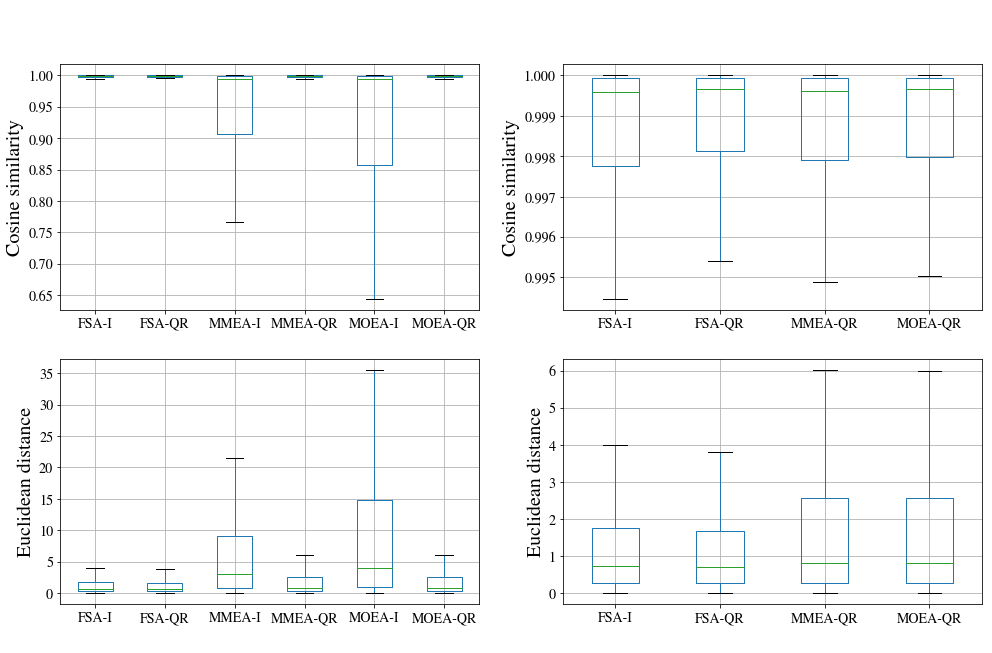
\includegraphics[width=14cm]{img/all_distances_feasible}

    \caption{Similarity of the solutions given by the algorithms finding $h$-element subsets satisfying strong necessary condition compared to the OLS solution on the subset of the data set that does not contain outliers. On the left are two box plots for all algorithms. Since the visualization is influenced by the scale of MMEA-I and MOEA-I box plots, we provide also two graphs without these two algorithms on the right.}
    \label{all_distances}
\end{figure}

\subsection{Algorithms for finding the exact solution}
Here we provide results of the algorithms finding the exact solution. For the improved versions of the BAB and BSA algorithms, which are able to incorporate pre-computed results, we decided to use the estimate given by the FSA-QR. This algorithm, as observed in previous section, provides the best results. FSA-QR is quite slow compared to the MOEA and MMEA variations, but because the exact algorithms have much higher time complexity (thus can be used only on very small data sets), this slowing down is insignificant with respect to the total time complexity.

The setup for the simulations was the same as in the previous section, but we only compare speed this time because all of the algorithms provide the exact solution. 

The results are given in Appendix~\ref{apendix:chapter} in Tables~\ref{table:exact:1}, \ref{table:exact:2} and \ref{table:exact:3} for data sets $D1$, $D2$ and $D3$ respectively. 
    
Interesting observation is given by the Figure~\ref{exact:improvement} depicting where is the average time of the calculation improved by the FSA-QR-BAB instead of the BAB and the FSA-QR-BSA instead of the BSA. Whereas FSA-QR-BAB improves the time of the computation significantly, the FSA-QR-BSA does not leads to any time improvement at all.
 
\begin{figure}[h]
    \centering
    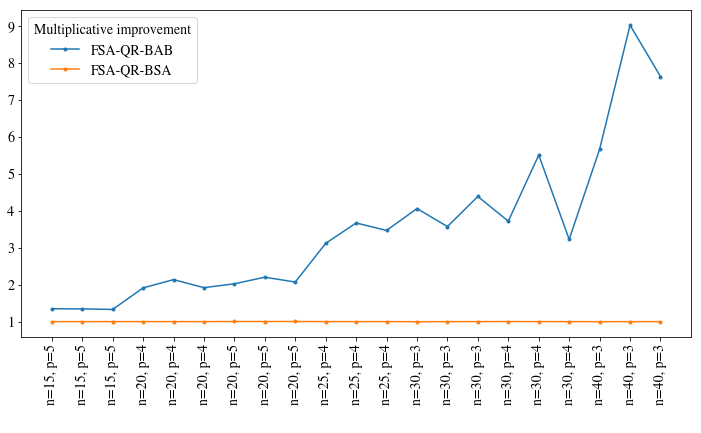
\includegraphics[width=12cm]{img/exact_improvement}

    \caption{For various combinations of parameters $n$ and $p$ we calculated average multiplicative improvement of the CPU time for running FSA-QR-BAB and FSA-QR-BSA instead of BAB and BSA.}
    \label{exact:improvement}

    
\end{figure}

We can observe from the results that BSA (as well as FSA-QR-BSA) is, as expected, sensitive to increasing the parameter $p$. On the other hand, when $p$ stays low, BSA outperforms both BAB and FSA-QR-BAB. We have ran $10$ simulations for higher values of $n$ for each dataset $D1$, $D2$ and $D3$ for algorithm BSA, while preserving value of $p = 2$. In this simulation we have not used intercept. Resulting average, minimum and maximum CPU times are given in Table~\ref{bsa:big:table}. For the data sets $D2$ and $D3$ the simulation was not performed for $n = 400$, so the 
respective cells are empty.


\begin{table}[h!]
    \centering

\scalebox{0.63}{
\begin{tabular}{l|l|l|r|r|r|r|r|r|r|r|r|} 
\hline\hline
&      & out & 
\multicolumn{3}{l|}{$D1$} &
\multicolumn{3}{l|}{$D2$} &
\multicolumn{3}{l|}{$D3$} \\  
\hline
$n$ & $out$ & $h$ &     avg &       min &       max &      avg &      min &      max &      avg &      min &      max \\
\hline
      100 & 0.10 & 51  &     5.499 &     5.213 &     6.860 &    5.206 &    5.150 &    5.273 &    5.215 &    5.166 &    5.342 \\    & 0.30 & 51  &     5.598 &     5.125 &     6.852 &    5.345 &    5.129 &    6.707 &    5.198 &    5.142 &    5.309 \\    & 0.45 & 51  &     5.978 &     5.161 &     6.902 &    5.347 &    5.099 &    6.724 &    5.425 &    5.164 &    6.989 \\200 & 0.10 & 101 &    81.172 &    80.042 &    81.582 &   81.280 &   80.816 &   81.575 &   82.678 &   81.153 &   93.849 \\    & 0.30 & 101 &    80.992 &    80.416 &    81.396 &   82.482 &   80.789 &   94.172 &   81.250 &   80.008 &   81.921 \\    & 0.45 & 101 &    81.101 &    80.660 &    82.054 &   81.165 &   80.836 &   81.496 &   81.332 &   81.088 &   81.631 \\300 & 0.10 & 151 &   422.982 &   421.551 &   423.973 &  425.611 &  422.521 &  466.379 &  423.312 &  422.593 &  424.112 \\    & 0.30 & 151 &   426.895 &   421.704 &   465.063 &  423.236 &  421.937 &  424.155 &  427.746 &  422.930 &  466.564 \\    & 0.45 & 151 &   427.169 &   421.060 &   467.341 &  427.391 &  421.636 &  466.195 &  423.404 &  422.699 &  424.172 \\400 & 0.10 & 201 &  1390.836 &  1378.586 &  1483.780 &      $-$ &      $-$ &      $-$ &      $-$ &      $-$ &      $-$ \\    & 0.30 & 201 &  1389.465 &  1373.600 &  1483.066 &      $-$ &      $-$ &      $-$ &      $-$ &      $-$ &      $-$ \\    & 0.45 & 201 &  1380.151 &  1373.839 &  1383.228 &      $-$ &      $-$ &      $-$ &      $-$ &      $-$ &      $-$ \\
\hline
\end{tabular}
% end table
}

\caption{Average, minimum and maximum CPU times of computation time for BSA for $p=2$ and various combinations of parameters $n$ and $out$  for each dataset.}
\label{bsa:big:table}

\end{table}


\subsection{FAST-LTS and combinations of the algorithms} \label{results:combinations}
In this section we present the results of the FAST-LTS algorithm compared to the MOEA-QR and MMEA-QR because, as described in Section~\ref{strong:experiments}, these algorithms seems to be very fast while providing reliable results. We also run simulations on the combinations of those two algorithms as described in Section~\ref{sectioncombined}. All algorithms were set to start from $50$ randomly chosen subsets for each simulation and maximum number of inner cycles was set to $40$. We ran simulations $100$ times for each combination of the parameters $n$, $p$ and $out$ for each data set. The results are given in Appendix~\ref{apendix:chapter} in Tables~\ref{table:combined:1}, \ref{table:combined:2} and \ref{table:combined:3} for data sets $D1$, $D2$ and $D3$ respectively. Beside measuring the cosine similarity and $L^2$ norm, we also provide the number of the inner cycles for each algorithms. We can see, that providing solution from the FAST-LTS to the MOEA-QR and MMEA-QR significantly reduce those numbers.
 
In Table~\ref{table:percentage:improvement} we can see that approximately in 30 $\%$ of cases MOEA-QR and MMEA-QR were able to improve the solution of the FAST-LTS in all three data sets. That means in those cases FAST-LTS algorithm have provided solutions that satisfied weak necessary condition but not the strong one. 

\begin{table}[h!]
    \centering
    \begin{tabular}{l|r|r|r|}
        \hline\hline
         &    $D1$ &    $D2$ &    $D3$ \\
         \hline
         FAST-LTS-MMEA-QR &  30.33 $\%$ &  34.00 $\%$ &  33.00 $\%$ \\FAST-LTS-MOEA-QR &  30.33 $\%$ &  35.33 $\%$ &  33.33 $\%$  \\
         \hline
         
    \end{tabular}

    \caption{Percentage of the $h$-elements subsets provided by FAST-LTS which did not satisfied strong necessary condition, and the MMEA-QR and MOEA-QR were able to improve them.}
    \label{table:percentage:improvement}
\end{table}

Let us note, that it would be interesting to exhaustively enumerate data sets and count number of $h$-element subsets which satisfies the weak and strong necessary conditions and, similarly, enumerate the ``domains'' of each such $h$-element subsets in terms how many $h$-elements subsets leads to the particular $h$-element subset satisfying the weak or strong necessary condition, respectively.


\subsection{Random algorithm and RBSA}
In Section~\ref{bsasection} we proposed the probabilistic version of BSA. We compare it to the Random solution algorithm (RANDOM) described in Section~\ref{first:attempts} and also to the FAST-LTS and MMEA-QR algorithms which were observed to provide efficient solutions in previous sections. In this experiments we set RANDOM and RBSA algorithm to start from $1000$ randomly chosen $(p+1)$-element subsets. FSA-LTS was set to start from $100$ $p$-element subsets and MMEA-QR from $100$ $h$-element subsets. Both algorithms were set to the maximum of $50$ inner cycles. For each combination of the parameters $n$, $p$ and $out$ we ran $10$ simulations. This was repeated for all three data sets. The results are given in Appendix~\ref{apendix:chapter} in Tables~\ref{table:randim:1}, \ref{table:randim:2} and \ref{table:randim:3} for data sets $D1$, $D2$ and $D3$, respectively, and include average CPU times, cosine similarity and $L^2$ norm in the same way as above.

\begin{figure}[h]
    \centering
    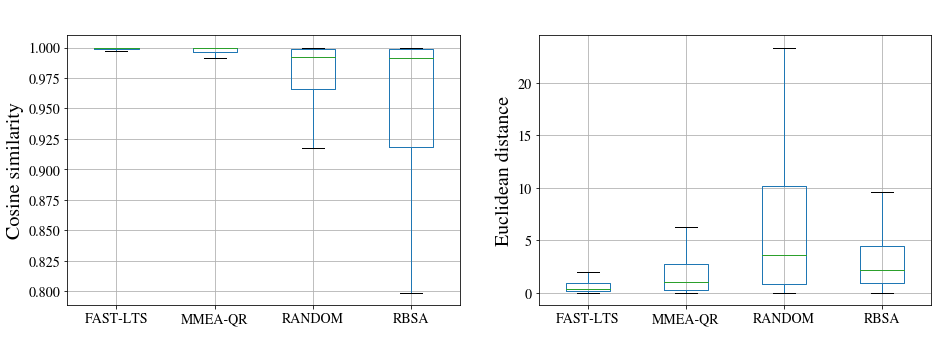
\includegraphics[width=12cm]{img/random_box}

    \caption{Cosine similarity and $L^2$ norm for multiple algorithms. Random algorithms are outperformed by the algorithms finding the weak and strong necessary conditions.}
    \label{randim:box}
\end{figure}

In Figure~\ref{randim:box} box plots describing the quality of the solution are given. The $L^2$ norm of the RBSA estimate is in average less, the cosine similarity is worse. Moreover we can clearly see that MMEA-QR and FAST-LTS provide much more reliable results (even in shorter CPU times).

There are many other possibilities for other experiments than what is provided in this chapter, especially the experiments suggested in the Section~\ref{results:combinations} for exploring domains of $h$-element subsets satisfying the weak and strong necessary conditions. These experiments are out of the scope of this work, because already provided simulations were quite exhaustive due to the lot of possible variations of the algorithms.  

\setsecnumdepth{part}

\chapter{Conclusion}
% Goal of this thesis was to compare probabilistic algorithms for computing the LTS estimate. 
We have surveyed, implemented and described multiple exact and probabilistic algorithms for calculating the LTS estimate.
Those algorithms have been proposed across the last few decades. Most recently proposed algorithms are just a few years old. This means that research in the filed of LTS algorithms is still ongoing.

Although the exact algorithms have polynomial time complexity, we showed that currently used probabilistic algorithm provide sufficiently fast solutions which, even though thay may not be exact, are good enough. Despite the fact that it was proven that the exact solution cannot be obtained faster than in polynomial time, we showed that currently used algorithms could be combined to obtain better results. 


Algorithms for calculating the LTS estimate are still open topic for further research. One of the possible research direction is to study possibility to combine the exact algorithms with probabilistic ones. As our experimental results suggest, we could possibly come up probabilistic algorithms which provide even better performance.

Another direction could be to use algorithms for computing LTS estimate on different robust statistic methods because some of them are very similar to the LTS problem.




% ******************************************************************
% ***********************  BIBLIOGRAPHY  ****************************
% ******************************************************************
% “book – A single-volume book with one or more authors where the authors share credit for the work as a whole.”

% “inbook – A part of a book which forms a self-contained unit with its own title. Note that the profile of this entry type is different from standard BibTeX, see § 2.3.1.”

% “collection – A single-volume collection with multiple, self-contained contributions by distinct authors which have their own title. The work as a whole has no overall author but it will usually have an editor.”

% “incollection – A contribution to a collection which forms a self-contained unit with a distinct author and title. The author refers to the title, the editor to the booktitle, i. e., the title of the collection.”

% INPROCEEDINGS - ???

% In practice, incollection items vastly outnumber inbook

\bibliographystyle{bib/iso690}
\bibliography{bib/mybibliographyfile}



% ******************************************************************
% ************************  APPENDIX  ******************************
% ******************************************************************
\setsecnumdepth{all}
\appendix

\chapter{Results of the experiments} \label{apendix:chapter}
%  Here we provide tabular results of the experiments from the Section~\ref{chapterexperiments} where you can find detailed description of experimental setup. 




%%%%%%%%%%%%%%%%%%%%%%%%%%%%%%%%%%%%%%%%%%%%%%%%%%%%%%%%%%%%%%%%%%%%%%%%%%%%%%%%%%%%%%%%%%%%%%%%%%%
%%%%%%%%%%%%%%%%%%%%%%%%%%%%%%%%%%%%%%%%%%%%%%%%%%%%%%%%%%%%%%%%%%%%%%%%%%%%%%%%%%%%%%%%%%%%%%%%%%%
%%%%%%%%%%%%%%%%%%%%%%%%%%%%%%%%%%%%%%%%%%%%%%%%%%%%%%%%%%%%%%%%%%%%%%%%%%%%%%%%%%%%%%%%%%%%%%%%%%%
%%%%%%%%%%%%%%%%%%%%%%%%%%%%%%%%%%%%%%%%%%%%%%%%%%%%%%%%%%%%%%%%%%%%%%%%%%%%%%%%%%%%%%%%%%%%%%%%%%%
%%%%%%%%%%%%%%%%%%%%%%%%%%%%%%%%%%%%%%%%%%%%%%%%%%%%%%%%%%%%%%%%%%%%%%%%%%%%%%%%%%%%%%%%%%%%%%%%%%%
 %%%%%%%%%%%%%%%%%%%%%%% STRONG CONDITION %%%%%%%%%%%%%%%%%%%%%%%%%%%%%%%%%%%%%%%%%%%%%%%%%%%%%%%%%
%%%%%%%%%%%%%%%%%%%%%%%%%%%%%%%%%%%%%%%%%%%%%%%%%%%%%%%%%%%%%%%%%%%%%%%%%%%%%%%%%%%%%%%%%%%%%%%%%%%
%%%%%%%%%%%%%%%%%%%%%%%%%%%%%%%%%%%%%%%%%%%%%%%%%%%%%%%%%%%%%%%%%%%%%%%%%%%%%%%%%%%%%%%%%%%%%%%%%%%
%%%%%%%%%%%%%%%%%%%%%%%%%%%%%%%%%%%%%%%%%%%%%%%%%%%%%%%%%%%%%%%%%%%%%%%%%%%%%%%%%%%%%%%%%%%%%%%%%%%
%%%%%%%%%%%%%%%%%%%%%%%%%%%%%%%%%%%%%%%%%%%%%%%%%%%%%%%%%%%%%%%%%%%%%%%%%%%%%%%%%%%%%%%%%%%%%%%%%%%
%%%%%%%%%%%%%%%%%%%%%%%%%%%%%%%%%%%%%%%%%%%%%%%%%%%%%%%%%%%%%%%%%%%%%%%%%%%%%%%%%%%%%%%%%%%%%%%%%%%



 %\section{Strong necessary condition algorithms results} \label{apendix:strong}




%%%%%%%%%%%%%%%%%%%%%%% TABLE 1 %%%%%%%%%%%%%%%%%%%%%%%%%%%%%%%%%%%%%%%%%%%%%%%%%%%%%%%%%%%%%%%
\begin{table}[h!]
    \centering
    
\begin{adjustbox}{angle=90}

% scale
% {\begin{adjustwidth}{-2.1cm}{0cm}

    \scalebox{0.63}{
    
    % tabular
    \begin{tabular}{l|l|l|l|r|r|r|r|r|r|r|r|r|r|r|r|r|r|r|r|r|r|}    
    \hline\hline         &    &      & alg & 
    \multicolumn{3}{l|}{FSA-I} & 
    \multicolumn{3}{l|}{FSA-QR} & 
    \multicolumn{3}{l|}{MMEA-I} & 
    \multicolumn{3}{l|}{MMEA-QR} & 
    \multicolumn{3}{l|}{MOEA-I} & 
    \multicolumn{3}{l|}{MOEA-QR} \\  
    \hline
    $n$ & $p$ & $out$ & $h$ &     time &    cos & l2 &   time &    cos &  l2 &   time &    cos & l2 &    time &    cos &  l2 &   time &    cos &  l2 &    time &    cos & l2 \\ 
    \hline
    20   & 3  & 0.10 & 12  &  0.000 &  0.983 &  1.496 &  0.007 &  0.991 &  1.475 &  0.000 &  0.895 &   4.693 &   0.000 &  0.990 &   1.488 &  0.000 &  0.699 &  23.235 &   0.000 &  0.988 &   1.447 \\     &    & 0.30 & 12  &  0.000 &  0.986 &  2.457 &  0.006 &  0.963 &  2.544 &  0.000 &  0.737 &  11.694 &   0.000 &  0.994 &   1.310 &  0.000 &  0.557 &  44.050 &   0.000 &  0.972 &   3.916 \\     &    & 0.45 & 12  &  0.000 &  0.848 &  8.643 &  0.004 &  0.947 &  4.337 &  0.000 &  0.652 &  20.731 &   0.000 &  0.916 &   5.594 &  0.000 &  0.594 &  37.565 &   0.000 &  0.863 &   6.180 \\100  & 4  & 0.10 & 52  &  0.020 &  0.998 &  0.855 &  0.179 &  0.998 &  0.965 &  0.001 &  0.965 &   2.710 &   0.003 &  0.998 &   0.978 &  0.003 &  0.877 &  11.660 &   0.006 &  0.998 &   0.836 \\     &    & 0.30 & 52  &  0.021 &  0.998 &  0.903 &  0.186 &  0.999 &  0.885 &  0.001 &  0.927 &   5.429 &   0.003 &  0.997 &   0.916 &  0.002 &  0.872 &  10.986 &   0.007 &  0.999 &   0.839 \\     &    & 0.45 & 52  &  0.021 &  0.999 &  0.611 &  0.151 &  0.999 &  0.656 &  0.001 &  0.939 &   6.489 &   0.003 &  0.999 &   0.653 &  0.002 &  0.880 &  11.619 &   0.007 &  0.998 &   0.640 \\     & 6  & 0.10 & 53  &  0.022 &  0.997 &  0.925 &  0.266 &  0.998 &  0.910 &  0.001 &  0.950 &   3.637 &   0.003 &  0.998 &   0.761 &  0.003 &  0.833 &  14.147 &   0.007 &  0.997 &   0.765 \\     &    & 0.30 & 53  &  0.024 &  0.997 &  0.887 &  0.286 &  0.998 &  0.914 &  0.001 &  0.915 &   6.815 &   0.003 &  0.998 &   0.854 &  0.003 &  0.831 &  17.549 &   0.008 &  0.997 &   0.975 \\     &    & 0.45 & 53  &  0.025 &  0.997 &  0.671 &  0.220 &  0.994 &  1.023 &  0.001 &  0.895 &   8.875 &   0.003 &  0.998 &   0.740 &  0.002 &  0.854 &  14.923 &   0.008 &  0.993 &   1.066 \\500  & 3  & 0.10 & 252 &  1.708 &  1.000 &  0.529 &  6.854 &  1.000 &  0.484 &  0.076 &  0.999 &   0.883 &   0.172 &  1.000 &   0.523 &  0.152 &  0.998 &   0.946 &   0.496 &  1.000 &   0.465 \\     &    & 0.30 & 252 &  1.662 &  1.000 &  1.176 &  6.661 &  1.000 &  1.153 &  0.076 &  0.997 &   1.973 &   0.173 &  1.000 &   1.194 &  0.157 &  0.997 &   2.053 &   0.489 &  1.000 &   1.217 \\     &    & 0.45 & 252 &  1.786 &  0.999 &  2.781 &  7.327 &  0.999 &  2.679 &  0.075 &  0.998 &   3.419 &   0.166 &  0.999 &   2.749 &  0.141 &  0.998 &   3.284 &   0.503 &  0.999 &   2.681 \\     & 6  & 0.10 & 253 &  2.014 &  1.000 &  0.421 &  8.535 &  1.000 &  0.366 &  0.076 &  0.994 &   1.117 &   0.162 &  1.000 &   0.375 &  0.112 &  0.994 &   1.411 &   0.481 &  1.000 &   0.430 \\     &    & 0.30 & 253 &  2.062 &  1.000 &  1.094 &  8.701 &  1.000 &  0.979 &  0.071 &  0.995 &   2.187 &   0.162 &  1.000 &   1.155 &  0.105 &  0.995 &   2.256 &   0.486 &  0.999 &   1.145 \\     &    & 0.45 & 253 &  2.077 &  0.999 &  2.632 &  8.866 &  0.999 &  2.464 &  0.068 &  0.994 &   3.868 &   0.153 &  0.999 &   2.602 &  0.104 &  0.994 &   3.735 &   0.484 &  0.999 &   2.719 \\1000 & 3  & 0.10 & 502 &    $-$ &    $-$ &    $-$ &    $-$ &    $-$ &    $-$ &  0.149 &  1.000 &   0.370 &   0.509 &  1.000 &   0.354 &  0.379 &  1.000 &   0.373 &   1.865 &  1.000 &   0.327 \\     &    & 0.30 & 502 &    $-$ &    $-$ &    $-$ &    $-$ &    $-$ &    $-$ &  0.147 &  0.999 &   3.021 &   0.367 &  0.999 &   3.029 &  0.265 &  1.000 &   2.911 &   1.665 &  1.000 &   2.909 \\     &    & 0.45 & 502 &    $-$ &    $-$ &    $-$ &    $-$ &    $-$ &    $-$ &  0.035 &  0.996 &  10.661 &   0.239 &  0.996 &  10.998 &  0.139 &  0.995 &  10.603 &   1.487 &  0.996 &  10.682 \\     & 6  & 0.10 & 503 &    $-$ &    $-$ &    $-$ &    $-$ &    $-$ &    $-$ &  0.172 &  1.000 &   0.455 &   0.585 &  1.000 &   0.345 &  0.360 &  1.000 &   0.486 &   1.895 &  1.000 &   0.349 \\     &    & 0.30 & 503 &    $-$ &    $-$ &    $-$ &    $-$ &    $-$ &    $-$ &  0.124 &  0.999 &   3.016 &   0.440 &  0.999 &   3.146 &  0.242 &  0.999 &   2.837 &   1.697 &  0.999 &   2.924 \\     &    & 0.45 & 503 &    $-$ &    $-$ &    $-$ &    $-$ &    $-$ &    $-$ &  0.030 &  0.994 &   8.955 &   0.345 &  0.994 &   9.092 &  0.143 &  0.994 &   8.933 &   1.562 &  0.993 &   9.095 \\     & 11 & 0.10 & 506 &    $-$ &    $-$ &    $-$ &    $-$ &    $-$ &    $-$ &  0.211 &  1.000 &   0.412 &   0.723 &  1.000 &   0.265 &  0.359 &  1.000 &   0.400 &   1.974 &  1.000 &   0.292 \\     &    & 0.30 & 506 &    $-$ &    $-$ &    $-$ &    $-$ &    $-$ &    $-$ &  0.094 &  0.999 &   2.708 &   0.616 &  0.999 &   2.657 &  0.230 &  0.999 &   2.622 &   1.874 &  0.999 &   2.559 \\     &    & 0.45 & 506 &    $-$ &    $-$ &    $-$ &    $-$ &    $-$ &    $-$ &  0.037 &  0.993 &   8.305 &   0.561 &  0.992 &   8.335 &  0.170 &  0.992 &   8.338 &   1.810 &  0.992 &   8.113 \\     & 21 & 0.10 & 511 &    $-$ &    $-$ &    $-$ &    $-$ &    $-$ &    $-$ &  0.204 &  1.000 &   0.449 &   1.186 &  1.000 &   0.294 &  0.457 &  1.000 &   0.577 &   2.719 &  1.000 &   0.315 \\     &    & 0.30 & 511 &    $-$ &    $-$ &    $-$ &    $-$ &    $-$ &    $-$ &  0.076 &  0.999 &   2.943 &   1.053 &  0.999 &   3.057 &  0.284 &  0.999 &   2.901 &   2.431 &  0.999 &   2.874 \\     &    & 0.45 & 511 &    $-$ &    $-$ &    $-$ &    $-$ &    $-$ &    $-$ &  0.051 &  0.989 &  10.646 &   1.018 &  0.991 &  11.064 &  0.280 &  0.991 &  10.797 &   2.464 &  0.991 &  10.594 \\
     
    \hline 
     \multicolumn{4}{l|}{\textbf{mean}} & 0.763 & 0.987 & 1.739 &	3.217 &	0.992 &	1.456 &	0.066 &	0.956 &	5.054 &	0.320 &	0.994 &	2.760 &	0.152 &	0.924 &	9.304 &	0.979 &	0.991 &	2.828 \\
    \hline 
    \end{tabular}    
    % end table
    
    
    }
    
    %\end{adjustwidth}  }
\end{adjustbox}
    % end scale
    
    \caption{Results of simulations for algorithms finding $h$-element subsets satisfying the strong necessary condition for the data set $D1$ for various configurations of the parameters $n$, $p$ and $out$. Results include average time and cosine similarity and $L^2$ norm.}
    \label{table1}
\end{table}


%%%%%%%%%%%%%%%%%%%%%%% TABLE 2 %%%%%%%%%%%%%%%%%%%%%%%%%%%%%%%%%%%%%%%%%%%%%%%%%%%%%%%%%%%%%%%
\begin{table}[h!]
    \centering


% scale
\begin{adjustbox}{angle=90}

%{\begin{adjustwidth}{-2.1cm}{0cm}

    \scalebox{0.63}{
    
    % tabular
    \begin{tabular}{l|l|l|l|r|r|r|r|r|r|r|r|r|r|r|r|r|r|r|r|r|r|}    
    \hline\hline         &    &      & alg & 
    \multicolumn{3}{l|}{FSA-I} & 
    \multicolumn{3}{l|}{FSA-QR} & 
    \multicolumn{3}{l|}{MMEA-I} & 
    \multicolumn{3}{l|}{MMEA-QR} & 
    \multicolumn{3}{l|}{MOEA-I} & 
    \multicolumn{3}{l|}{MOEA-QR} \\  
    \hline
    $n$ & $p$ & $out$ & $h$ &     time &    cos & l2 &   time &    cos &  l2 &   time &    cos & l2 &    time &    cos &  l2 &   time &    cos &  l2 &    time &    cos & l2 \\ 
    \hline
    
    20   & 3  & 0.10 & 12  &  0.000 &  0.990 &   1.945 &  0.006 &  0.992 &   1.973 &  0.000 &  0.888 &   7.989 &   0.000 &  0.993 &   1.645 &  0.000 &  0.734 &  35.866 &   0.000 &  0.992 &   1.733 \\     &    & 0.30 & 12  &  0.000 &  0.870 &   9.287 &  0.006 &  0.883 &  10.860 &  0.000 &  0.582 &  23.583 &   0.000 &  0.869 &  11.504 &  0.000 &  0.506 &  47.430 &   0.000 &  0.953 &   7.286 \\     &    & 0.45 & 12  &  0.000 &  0.691 &  21.370 &  0.004 &  0.749 &  16.951 &  0.000 &  0.545 &  32.270 &   0.000 &  0.716 &  17.784 &  0.000 &  0.533 &  38.293 &   0.000 &  0.732 &  17.072 \\100  & 4  & 0.10 & 52  &  0.019 &  0.998 &   0.984 &  0.165 &  0.998 &   0.943 &  0.001 &  0.771 &   8.848 &   0.003 &  0.998 &   0.937 &  0.003 &  0.621 &  27.151 &   0.006 &  0.998 &   1.041 \\     &    & 0.30 & 52  &  0.021 &  0.983 &   1.930 &  0.203 &  0.983 &   1.809 &  0.001 &  0.699 &  17.484 &   0.003 &  0.995 &   2.020 &  0.003 &  0.681 &  32.773 &   0.007 &  0.992 &   1.485 \\     &    & 0.45 & 52  &  0.019 &  0.837 &   9.497 &  0.123 &  0.830 &  11.490 &  0.001 &  0.677 &  30.080 &   0.003 &  0.894 &   7.186 &  0.003 &  0.660 &  35.166 &   0.006 &  0.894 &   8.129 \\     & 6  & 0.10 & 53  &  0.021 &  0.997 &   0.863 &  0.271 &  0.998 &   0.835 &  0.001 &  0.689 &  20.252 &   0.003 &  0.998 &   0.861 &  0.004 &  0.572 &  48.255 &   0.007 &  0.998 &   0.904 \\     &    & 0.30 & 53  &  0.025 &  0.986 &   3.821 &  0.290 &  0.972 &   4.816 &  0.001 &  0.672 &  34.943 &   0.003 &  0.996 &   1.514 &  0.004 &  0.670 &  49.795 &   0.008 &  0.991 &   2.085 \\     &    & 0.45 & 53  &  0.025 &  0.892 &  18.193 &  0.189 &  0.896 &  19.771 &  0.001 &  0.627 &  58.788 &   0.003 &  0.883 &  20.926 &  0.004 &  0.662 &  81.034 &   0.008 &  0.908 &  15.608 \\500  & 3  & 0.10 & 252 &  1.644 &  1.000 &   0.420 &  6.933 &  1.000 &   0.452 &  0.014 &  0.936 &   1.525 &   0.072 &  1.000 &   0.439 &  0.041 &  0.930 &   1.919 &   0.402 &  1.000 &   0.451 \\     &    & 0.30 & 252 &  1.669 &  0.999 &   0.547 &  7.049 &  1.000 &   0.540 &  0.014 &  0.814 &   4.182 &   0.074 &  0.999 &   0.603 &  0.043 &  0.821 &   4.607 &   0.415 &  1.000 &   0.593 \\     &    & 0.45 & 252 &  1.744 &  0.863 &   7.336 &  7.205 &  0.910 &   4.894 &  0.015 &  0.693 &  14.545 &   0.078 &  0.888 &   8.072 &  0.043 &  0.725 &  14.494 &   0.422 &  0.920 &   5.066 \\     & 6  & 0.10 & 253 &  2.001 &  0.999 &   0.507 &  8.659 &  1.000 &   0.493 &  0.015 &  0.879 &   5.676 &   0.104 &  0.999 &   0.421 &  0.048 &  0.848 &   8.561 &   0.435 &  0.999 &   0.463 \\     &    & 0.30 & 253 &  2.095 &  0.999 &   3.193 &  8.913 &  0.999 &   3.078 &  0.015 &  0.817 &  16.367 &   0.107 &  1.000 &   3.148 &  0.047 &  0.820 &  17.580 &   0.446 &  1.000 &   2.929 \\     &    & 0.45 & 253 &  2.049 &  0.922 &  13.144 &  8.838 &  0.916 &  14.667 &  0.015 &  0.769 &  44.826 &   0.107 &  0.911 &  14.810 &  0.043 &  0.768 &  43.490 &   0.433 &  0.906 &  15.377 \\1000 & 3  & 0.10 & 502 &    $-$ &    $-$ &     $-$ &    $-$ &    $-$ &     $-$ &  0.027 &  1.000 &   0.278 &   0.237 &  1.000 &   0.236 &  0.134 &  1.000 &   0.253 &   1.478 &  1.000 &   0.249 \\     &    & 0.30 & 502 &    $-$ &    $-$ &     $-$ &    $-$ &    $-$ &     $-$ &  0.029 &  0.999 &   0.634 &   0.267 &  1.000 &   0.653 &  0.146 &  1.000 &   0.654 &   1.582 &  1.000 &   0.647 \\     &    & 0.45 & 502 &    $-$ &    $-$ &     $-$ &    $-$ &    $-$ &     $-$ &  0.030 &  0.811 &   1.996 &   0.282 &  0.728 &   1.775 &  0.149 &  0.878 &   1.969 &   1.598 &  0.821 &   1.972 \\     & 6  & 0.10 & 503 &    $-$ &    $-$ &     $-$ &    $-$ &    $-$ &     $-$ &  0.030 &  1.000 &   0.306 &   0.348 &  1.000 &   0.255 &  0.146 &  1.000 &   0.298 &   1.571 &  1.000 &   0.285 \\     &    & 0.30 & 503 &    $-$ &    $-$ &     $-$ &    $-$ &    $-$ &     $-$ &  0.032 &  1.000 &   1.634 &   0.391 &  1.000 &   1.633 &  0.155 &  1.000 &   1.659 &   1.665 &  1.000 &   1.648 \\     &    & 0.45 & 503 &    $-$ &    $-$ &     $-$ &    $-$ &    $-$ &     $-$ &  0.035 &  0.748 &   5.133 &   0.439 &  0.705 &   4.894 &  0.158 &  0.708 &   5.064 &   1.728 &  0.686 &   4.304 \\     & 11 & 0.10 & 506 &    $-$ &    $-$ &     $-$ &    $-$ &    $-$ &     $-$ &  0.037 &  1.000 &   0.311 &   0.559 &  1.000 &   0.301 &  0.184 &  1.000 &   0.345 &   1.820 &  1.000 &   0.301 \\     &    & 0.30 & 506 &    $-$ &    $-$ &     $-$ &    $-$ &    $-$ &     $-$ &  0.038 &  0.977 &   4.805 &   0.584 &  0.980 &   3.649 &  0.181 &  0.983 &   4.620 &   1.849 &  0.992 &   3.478 \\     &    & 0.45 & 506 &    $-$ &    $-$ &     $-$ &    $-$ &    $-$ &     $-$ &  0.039 &  0.739 &   8.669 &   0.616 &  0.711 &   7.955 &  0.175 &  0.781 &   8.871 &   1.868 &  0.763 &   8.356 \\     & 21 & 0.10 & 511 &    $-$ &    $-$ &     $-$ &    $-$ &    $-$ &     $-$ &  0.053 &  0.999 &   0.432 &   1.024 &  1.000 &   0.277 &  0.294 &  0.993 &   0.683 &   2.579 &  1.000 &   0.326 \\     &    & 0.30 & 511 &    $-$ &    $-$ &     $-$ &    $-$ &    $-$ &     $-$ &  0.055 &  0.903 &  13.742 &   1.115 &  0.933 &   9.280 &  0.294 &  0.903 &  13.823 &   2.512 &  0.945 &   9.462 \\     &    & 0.45 & 511 &    $-$ &    $-$ &     $-$ &    $-$ &    $-$ &     $-$ &  0.055 &  0.646 &  15.593 &   1.151 &  0.626 &  13.667 &  0.279 &  0.645 &  15.189 &   2.610 &  0.609 &  13.806 \\
    
    \hline 
     \multicolumn{4}{l|}{\textbf{mean}} & 0.756 &	0.935 &	6.202 &	3.257 &	0.942 &	6.238 &	0.021 &	0.810 &	13.885 &	0.281 &	0.919 &	5.053 &	0.096 &	0.794 &	19.994 &	0.943 &	0.930 &	4.632 \\
    \hline 
    \end{tabular}    
    % end table
    
    }
    
    % \end{adjustwidth}  }
    % end scale
\end{adjustbox}
    
\caption{Results of simulations for algorithms finding $h$-element subsets satisfying the strong necessary condition for the data set $D2$ for various configurations of the parameters $n$, $p$ and $out$. Results include average time and cosine similarity and $L^2$ norm.}
    \label{table2}
\end{table}



%%%%%%%%%%%%%%%%%%%%%%% TABLE 3 %%%%%%%%%%%%%%%%%%%%%%%%%%%%%%%%%%%%%%%%%%%%%%%%%%%%%%%%%%%%%%%
\begin{table}[h!]
    \centering
    

% scale
% {\begin{adjustwidth}{-2.1cm}{0cm}
    \begin{adjustbox}{angle=90}

    \scalebox{0.63}{
    
    % tabular
    \begin{tabular}{l|l|l|l|r|r|r|r|r|r|r|r|r|r|r|r|r|r|r|r|r|r|}    
    \hline\hline         &    &      & alg & 
    \multicolumn{3}{l|}{FSA-I} & 
    \multicolumn{3}{l|}{FSA-QR} & 
    \multicolumn{3}{l|}{MMEA-I} & 
    \multicolumn{3}{l|}{MMEA-QR} & 
    \multicolumn{3}{l|}{MOEA-I} & 
    \multicolumn{3}{l|}{MOEA-QR} \\  
    \hline
    $n$ & $p$ & $out$ & $h$ &     time &    cos & l2 &   time &    cos &  l2 &   time &    cos & l2 &    time &    cos &  l2 &   time &    cos &  l2 &    time &    cos & l2 \\ 
    \hline
    20   & 3  & 0.10 & 12  &  0.000 &  0.987 &  1.648 &  0.007 &  0.993 &  1.584 &  0.000 &  0.850 &   9.931 &   0.000 &  0.992 &   1.505 &  0.000 &  0.625 &  37.956 &   0.000 &  0.990 &   1.749 \\     &    & 0.30 & 12  &  0.000 &  0.978 &  2.893 &  0.007 &  0.980 &  2.322 &  0.000 &  0.595 &  23.852 &   0.000 &  0.957 &   2.431 &  0.000 &  0.440 &  55.069 &   0.000 &  0.973 &   3.275 \\     &    & 0.45 & 12  &  0.000 &  0.855 &  9.627 &  0.003 &  0.898 &  8.978 &  0.000 &  0.641 &  26.917 &   0.000 &  0.889 &  10.512 &  0.000 &  0.621 &  43.391 &   0.000 &  0.910 &  13.152 \\100  & 4  & 0.10 & 52  &  0.021 &  0.998 &  1.030 &  0.192 &  0.998 &  0.916 &  0.001 &  0.917 &   4.816 &   0.003 &  0.998 &   0.877 &  0.004 &  0.757 &  24.437 &   0.007 &  0.998 &   0.956 \\     &    & 0.30 & 52  &  0.021 &  0.998 &  0.849 &  0.197 &  0.998 &  0.795 &  0.001 &  0.752 &  10.570 &   0.003 &  0.997 &   0.811 &  0.003 &  0.684 &  28.215 &   0.007 &  0.998 &   0.789 \\     &    & 0.45 & 52  &  0.023 &  0.999 &  0.564 &  0.155 &  0.999 &  0.554 &  0.001 &  0.778 &  13.069 &   0.003 &  0.999 &   0.535 &  0.003 &  0.742 &  22.952 &   0.008 &  0.999 &   0.561 \\     & 6  & 0.10 & 53  &  0.023 &  0.997 &  1.075 &  0.291 &  0.997 &  0.943 &  0.001 &  0.723 &  15.112 &   0.003 &  0.997 &   0.876 &  0.004 &  0.625 &  39.288 &   0.008 &  0.997 &   0.942 \\     &    & 0.30 & 53  &  0.024 &  0.997 &  0.746 &  0.271 &  0.998 &  0.740 &  0.001 &  0.674 &  21.592 &   0.003 &  0.997 &   1.111 &  0.004 &  0.603 &  51.948 &   0.008 &  0.998 &   0.779 \\     &    & 0.45 & 53  &  0.027 &  0.999 &  0.616 &  0.240 &  0.996 &  1.404 &  0.001 &  0.642 &  40.547 &   0.004 &  0.997 &   1.006 &  0.004 &  0.645 &  52.690 &   0.009 &  0.997 &   0.759 \\500  & 3  & 0.10 & 252 &  1.736 &  1.000 &  0.495 &  7.368 &  1.000 &  0.439 &  0.015 &  0.974 &   1.041 &   0.077 &  1.000 &   0.495 &  0.045 &  0.925 &   1.754 &   0.424 &  1.000 &   0.503 \\     &    & 0.30 & 252 &  1.625 &  1.000 &  0.930 &  6.812 &  1.000 &  0.838 &  0.014 &  0.951 &   3.346 &   0.070 &  0.999 &   0.868 &  0.040 &  0.958 &   2.699 &   0.395 &  1.000 &   0.948 \\     &    & 0.45 & 252 &  1.712 &  0.999 &  2.197 &  7.186 &  0.999 &  2.046 &  0.015 &  0.924 &   4.274 &   0.074 &  0.999 &   2.124 &  0.042 &  0.908 &   4.275 &   0.413 &  1.000 &   2.088 \\     & 6  & 0.10 & 253 &  2.114 &  0.999 &  0.469 &  9.017 &  1.000 &  0.440 &  0.016 &  0.931 &   2.587 &   0.110 &  0.999 &   0.472 &  0.052 &  0.791 &   8.573 &   0.448 &  0.999 &   0.480 \\     &    & 0.30 & 253 &  2.138 &  1.000 &  0.964 &  9.101 &  1.000 &  0.951 &  0.016 &  0.898 &   6.597 &   0.110 &  1.000 &   1.054 &  0.049 &  0.873 &   8.730 &   0.456 &  1.000 &   1.035 \\     &    & 0.45 & 253 &  2.044 &  0.999 &  2.216 &  8.850 &  0.999 &  1.986 &  0.015 &  0.853 &   9.545 &   0.107 &  0.999 &   2.201 &  0.044 &  0.872 &   8.614 &   0.434 &  0.999 &   2.160 \\1000 & 3  & 0.10 & 502 &    $-$ &    $-$ &    $-$ &    $-$ &    $-$ &    $-$ &  0.030 &  1.000 &   0.321 &   0.299 &  1.000 &   0.279 &  0.152 &  1.000 &   0.295 &   1.645 &  1.000 &   0.278 \\     &    & 0.30 & 502 &    $-$ &    $-$ &    $-$ &    $-$ &    $-$ &    $-$ &  0.030 &  1.000 &   1.132 &   0.323 &  1.000 &   1.081 &  0.154 &  1.000 &   1.041 &   1.688 &  1.000 &   1.060 \\     &    & 0.45 & 502 &    $-$ &    $-$ &    $-$ &    $-$ &    $-$ &    $-$ &  0.163 &  0.998 &   3.358 &   0.520 &  0.998 &   3.559 &  0.401 &  0.998 &   3.452 &   1.774 &  0.999 &   3.469 \\     & 6  & 0.10 & 503 &    $-$ &    $-$ &    $-$ &    $-$ &    $-$ &    $-$ &  0.032 &  1.000 &   0.366 &   0.427 &  1.000 &   0.285 &  0.157 &  0.999 &   0.417 &   1.702 &  1.000 &   0.307 \\     &    & 0.30 & 503 &    $-$ &    $-$ &    $-$ &    $-$ &    $-$ &    $-$ &  0.032 &  1.000 &   1.856 &   0.418 &  1.000 &   1.688 &  0.155 &  1.000 &   1.772 &   1.707 &  1.000 &   1.755 \\     &    & 0.45 & 503 &    $-$ &    $-$ &    $-$ &    $-$ &    $-$ &    $-$ &  0.183 &  0.996 &   5.619 &   0.596 &  0.996 &   5.572 &  0.368 &  0.997 &   5.583 &   1.823 &  0.996 &   5.515 \\     & 11 & 0.10 & 506 &    $-$ &    $-$ &    $-$ &    $-$ &    $-$ &    $-$ &  0.038 &  1.000 &   0.380 &   0.645 &  1.000 &   0.265 &  0.183 &  0.999 &   0.362 &   1.936 &  1.000 &   0.259 \\     &    & 0.30 & 506 &    $-$ &    $-$ &    $-$ &    $-$ &    $-$ &    $-$ &  0.037 &  0.999 &   2.249 &   0.596 &  0.999 &   2.330 &  0.175 &  0.999 &   2.364 &   1.877 &  0.999 &   2.172 \\     &    & 0.45 & 506 &    $-$ &    $-$ &    $-$ &    $-$ &    $-$ &    $-$ &  0.210 &  0.993 &   8.146 &   0.752 &  0.993 &   8.049 &  0.358 &  0.992 &   8.073 &   1.950 &  0.992 &   8.198 \\     & 21 & 0.10 & 511 &    $-$ &    $-$ &    $-$ &    $-$ &    $-$ &    $-$ &  0.055 &  0.999 &   0.462 &   1.239 &  1.000 &   0.356 &  0.279 &  0.997 &   0.554 &   2.785 &  1.000 &   0.321 \\     &    & 0.30 & 511 &    $-$ &    $-$ &    $-$ &    $-$ &    $-$ &    $-$ &  0.053 &  0.997 &   3.195 &   1.132 &  0.999 &   2.661 &  0.271 &  0.996 &   3.057 &   2.530 &  0.999 &   2.730 \\     &    & 0.45 & 511 &    $-$ &    $-$ &    $-$ &    $-$ &    $-$ &    $-$ &  0.206 &  0.968 &  13.257 &   1.212 &  0.971 &  12.368 &  0.436 &  0.969 &  12.822 &   2.614 &  0.971 &  12.274 \\
    
    \hline 
     \multicolumn{4}{l|}{\textbf{mean}} 
     & 0.767 &	0.987 &	1.755 &	3.313 &	0.990 &	1.662 &	0.043 &	0.891 &	8.672 &	0.323 &	0.992 &	2.421 &	0.125 &	0.852 &	15.940 &	0.987 &	0.993 &	2.538 \\
    \hline 
    \end{tabular}    
    % end table
    
    
    
    }
    
    %\end{adjustwidth}   }
    % end scale
\end{adjustbox}
    
\caption{Results of simulations for algorithms finding $h$-element subsets satisfying the strong necessary condition for the data set $D3$ for various configurations of the parameters $n$, $p$ and $out$. Results include average time and cosine similarity and $L^2$ norm.}
    \label{table3}
\end{table}







%%%%%%%%%%%%%%%%%%%%%%%%%%%%%%%%%%%%%%%%%%%%%%%%%%%%%%%%%%%%%%%%%%%%%%%%%%%%%%%%%%%%%%%%%%%%%%%%%%%%%%%%%%%%%%%%%%%%%%%%%%%%%%%%%%%%%%%%%%%%%%%%%%%%%%%%%%%%%%%%%%%%%%%%%%%%%%%%%%%%%%%%%%%%%%%%%%%%%%%%
%%%%%%%%%%%%%%%%%%%%%%%%%%%%%%%%%%%%%%%%%%%%%%%%%%%%%%%%%%%%%%%%%%%%%%%%%%%%%%%%%%%%%%%%%%%%%%%%%%%%
%%%%%%%%%%%%%%%%%%%%%%%%%%%%%%%%%%%%%%%%%%%%%%%%%%%%%%%%%%%%%%%%%%%%%%%%%%%%%%%%%%%%%%%%%%%%%%%%%%%%
%%%%%%%%%%%%%%%%%%%%%%%%%%%%%%%%%%%%%%%%%%%%%%%%%%%%%%%%%%%%%%%%%%%%%%%%%%%%%%%%%%%%%%%%%%%%%%%%%%%%
%%%%%%%%%%%%%%%%%%%%%%%%%%%%%%%%%%%%%%%%%%%%%%%%%%%%%%%%%%%%%%%%%%%%%%%%%%%%%%%%%%%%%%%%%%%%%%%%%%%%
%%%%%%%%%%%%%%%%%%%%%%%%%%%%%%%%%%%%%%%%%%%%%%%%%%%%%%%%%%%%%%%%%%%%%%%%%%%%%%%%%%%%%%%%%%%%%%%%%%%%

   
%%%%%%%%%%%%%%%%%%%%%%% TABLE exact 1 %%%%%%%%%%%%%%%%%%%%%%%%%%%%%%%%%%%%%%%%%%%%%%%%%%%%%%%%%%%%
\begin{table}[h!]
    \centering
    

% scale
% {\begin{adjustwidth}{-2.1cm}{0cm}
    \begin{adjustbox}{angle=90}


		\scalebox{0.63}{

			\begin{tabular}{l|l|l|l|r|r|r|r|r|r|r|r|r|r|r|r|r|r|r|}
			\hline\hline
			&   &      & alg & 
			\multicolumn{3}{l|}{BAB} &
			\multicolumn{3}{l|}{BSA} &
			\multicolumn{3}{l|}{EXACT} & 
			\multicolumn{3}{l|}{FSA-QR-BAB} & 
			\multicolumn{3}{l|}{FSA-QR-BSA} \\ 
			\hline
			$n$ & $p$ & $out$ & $h$ &     avg &     min &      max &     avg &     min &     max &     avg &     min &     max &         avg &    min &     max &         avg &     min &     max \\
			\hline
			 15 & 5 & 0.10 & 10 &    0.003 &   0.002 &    0.005 &   2.362 &   1.873 &   2.944 &    0.008 &    0.007 &    0.014 &       0.002 &  0.001 &   0.004 &       2.363 &   1.811 &   3.358 \\   &   & 0.30 & 10 &    0.002 &   0.002 &    0.003 &   2.063 &   1.777 &   2.476 &    0.008 &    0.007 &    0.008 &       0.002 &  0.001 &   0.003 &       2.061 &   1.773 &   2.486 \\   &   & 0.45 & 10 &    0.003 &   0.002 &    0.005 &   2.040 &   1.781 &   2.425 &    0.007 &    0.007 &    0.008 &       0.002 &  0.001 &   0.004 &       2.045 &   1.782 &   2.438 \\20 & 4 & 0.10 & 12 &    0.017 &   0.012 &    0.034 &   1.839 &   1.744 &   1.994 &    0.283 &    0.278 &    0.306 &       0.009 &  0.004 &   0.019 &       1.838 &   1.764 &   1.994 \\   &   & 0.30 & 12 &    0.016 &   0.012 &    0.025 &   1.868 &   1.740 &   2.040 &    0.290 &    0.272 &    0.327 &       0.007 &  0.004 &   0.020 &       1.866 &   1.732 &   2.032 \\   &   & 0.45 & 12 &    0.014 &   0.011 &    0.027 &   1.855 &   1.751 &   2.019 &    0.289 &    0.272 &    0.307 &       0.007 &  0.003 &   0.016 &       1.851 &   1.743 &   1.995 \\   & 5 & 0.10 & 13 &    0.022 &   0.018 &    0.036 &  13.814 &  12.808 &  15.674 &    0.204 &    0.194 &    0.217 &       0.010 &  0.005 &   0.022 &      13.766 &  12.676 &  15.680 \\   &   & 0.30 & 13 &    0.021 &   0.017 &    0.033 &  13.441 &  12.564 &  14.544 &    0.204 &    0.194 &    0.238 &       0.009 &  0.004 &   0.017 &      13.389 &  12.593 &  14.420 \\   &   & 0.45 & 13 &    0.020 &   0.017 &    0.030 &  13.577 &  12.651 &  14.664 &    0.206 &    0.193 &    0.234 &       0.009 &  0.005 &   0.020 &      13.525 &  12.610 &  14.626 \\25 & 4 & 0.10 & 15 &    0.208 &   0.099 &    0.563 &   7.706 &   5.996 &  14.464 &    9.814 &    7.242 &   16.872 &       0.066 &  0.011 &   0.350 &       7.689 &   5.986 &  14.861 \\   &   & 0.30 & 15 &    0.180 &   0.096 &    0.437 &   7.737 &   5.974 &   9.681 &    9.491 &    7.314 &   11.406 &       0.047 &  0.009 &   0.277 &       7.734 &   5.882 &   9.633 \\   &   & 0.45 & 15 &    0.196 &   0.143 &    0.400 &   9.097 &   8.950 &   9.402 &   11.213 &   11.081 &   11.324 &       0.049 &  0.013 &   0.139 &       9.076 &   8.831 &   9.421 \\30 & 3 & 0.10 & 17 &    1.709 &   0.806 &    3.700 &   1.485 &   1.437 &   2.433 &  368.801 &  366.077 &  375.885 &       0.427 &  0.067 &   1.500 &       1.489 &   1.437 &   2.432 \\   &   & 0.30 & 17 &    1.189 &   0.743 &    2.176 &   1.494 &   1.478 &   1.518 &      $-$ &      $-$ &      $-$ &       0.305 &  0.135 &   0.722 &       1.495 &   1.472 &   1.531 \\   &   & 0.45 & 17 &    1.064 &   0.731 &    2.929 &   1.491 &   1.472 &   1.536 &      $-$ &      $-$ &      $-$ &       0.190 &  0.040 &   0.523 &       1.487 &   1.471 &   1.508 \\   & 4 & 0.10 & 17 &    1.733 &   0.858 &    3.440 &  24.221 &  24.009 &  24.645 &      $-$ &      $-$ &      $-$ &       0.389 &  0.117 &   1.063 &      24.083 &  23.932 &  24.228 \\   &   & 0.30 & 17 &    1.110 &   0.519 &    1.840 &  24.131 &  23.817 &  24.388 &      $-$ &      $-$ &      $-$ &       0.202 &  0.086 &   0.370 &      24.133 &  23.875 &  24.392 \\   &   & 0.45 & 17 &    0.908 &   0.717 &    1.545 &  24.107 &  23.750 &  24.265 &      $-$ &      $-$ &      $-$ &       0.384 &  0.067 &   0.948 &      24.109 &  23.782 &  24.421 \\40 & 3 & 0.10 & 22 &  103.891 &  58.453 &  183.988 &   9.986 &   8.386 &  11.580 &      $-$ &      $-$ &      $-$ &      16.839 &  2.723 &  43.747 &       9.999 &   8.386 &  11.617 \\   &   & 0.30 & 22 &   78.415 &  42.544 &  118.603 &   8.397 &   8.316 &   8.445 &      $-$ &      $-$ &      $-$ &       6.615 &  0.864 &  26.232 &       8.402 &   8.377 &   8.434 \\   &   & 0.45 & 22 &   37.435 &  22.998 &   66.874 &   8.404 &   8.338 &   8.442 &      $-$ &      $-$ &      $-$ &      10.809 &  0.273 &  55.871 &       8.409 &   8.340 &   8.454 \\
			 \hline 
			\end{tabular} 
			% end table
			
			
			
			}
			
    %\end{adjustwidth}   }
    % end scale
\end{adjustbox}
    
    \caption{Average, minimum and maximum CPU times of simulations for exact algorithms for the data set $D1$ for various configurations of the parameters $n$, $p$ and $out$.}
    \label{table:exact:1}
\end{table}




   
%%%%%%%%%%%%%%%%%%%%%%% TABLE exact 2 %%%%%%%%%%%%%%%%%%%%%%%%%%%%%%%%%%%%%%%%%%%%%%%%%%%%%%%%%%%%
\begin{table}[h!]
    \centering
    

% scale
% {\begin{adjustwidth}{-2.1cm}{0cm}
    \begin{adjustbox}{angle=90}


		\scalebox{0.63}{

			\begin{tabular}{l|l|l|l|r|r|r|r|r|r|r|r|r|r|r|r|r|r|r|}
			\hline\hline
			&   &      & alg & 
			\multicolumn{3}{l|}{BAB} &
			\multicolumn{3}{l|}{BSA} &
			\multicolumn{3}{l|}{EXACT} & 
			\multicolumn{3}{l|}{FSA-QR-BAB} & 
			\multicolumn{3}{l|}{FSA-QR-BSA} \\ 
			\hline
			$n$ & $p$ & $out$ & $h$ &     avg &     min &      max &     avg &     min &     max &     avg &     min &     max &         avg &    min &     max &         avg &     min &     max \\
			\hline
			15 & 5 & 0.10 & 10 &    0.003 &   0.002 &    0.004 &   2.132 &   1.782 &   2.648 &   0.008 &   0.007 &   0.010 &       0.002 &  0.001 &   0.003 &       2.130 &   1.782 &   2.660 \\   &   & 0.30 & 10 &    0.003 &   0.002 &    0.004 &   2.105 &   1.794 &   2.460 &   0.008 &   0.007 &   0.012 &       0.002 &  0.001 &   0.003 &       2.104 &   1.770 &   2.487 \\   &   & 0.45 & 10 &    0.003 &   0.002 &    0.004 &   2.154 &   1.801 &   2.543 &   0.008 &   0.007 &   0.010 &       0.002 &  0.002 &   0.004 &       2.149 &   1.801 &   2.535 \\20 & 4 & 0.10 & 12 &    0.018 &   0.013 &    0.033 &   1.922 &   1.851 &   2.026 &   0.297 &   0.277 &   0.335 &       0.010 &  0.004 &   0.018 &       1.923 &   1.808 &   2.051 \\   &   & 0.30 & 12 &    0.017 &   0.012 &    0.025 &   1.860 &   1.744 &   2.022 &   0.288 &   0.271 &   0.314 &       0.009 &  0.004 &   0.022 &       1.863 &   1.747 &   2.037 \\   &   & 0.45 & 12 &    0.016 &   0.012 &    0.024 &   1.829 &   1.749 &   2.006 &   0.283 &   0.270 &   0.329 &       0.008 &  0.003 &   0.017 &       1.831 &   1.755 &   2.053 \\   & 5 & 0.10 & 13 &    0.022 &   0.017 &    0.035 &  13.544 &  12.781 &  14.983 &   0.200 &   0.193 &   0.218 &       0.011 &  0.005 &   0.023 &      13.476 &  12.739 &  14.920 \\   &   & 0.30 & 13 &    0.021 &   0.017 &    0.033 &  13.388 &  12.676 &  14.732 &   0.201 &   0.194 &   0.275 &       0.010 &  0.005 &   0.021 &      13.337 &  12.656 &  14.594 \\   &   & 0.45 & 13 &    0.022 &   0.017 &    0.037 &  13.584 &  12.720 &  15.150 &   0.202 &   0.194 &   0.216 &       0.011 &  0.006 &   0.022 &      13.534 &  12.713 &  15.235 \\25 & 4 & 0.10 & 15 &    0.260 &   0.152 &    0.449 &   9.144 &   8.960 &   9.384 &  11.217 &  11.048 &  11.369 &       0.089 &  0.024 &   0.267 &       9.155 &   8.923 &   9.773 \\   &   & 0.30 & 15 &    0.250 &   0.149 &    0.549 &   9.118 &   8.928 &   9.335 &  11.224 &  11.009 &  11.370 &       0.071 &  0.019 &   0.206 &       9.108 &   8.952 &   9.309 \\   &   & 0.45 & 15 &    0.230 &   0.144 &    0.398 &   9.106 &   8.808 &   9.372 &  11.225 &  11.112 &  11.331 &       0.076 &  0.021 &   0.289 &       9.110 &   8.901 &  10.166 \\30 & 3 & 0.10 & 17 &    1.555 &   0.975 &    2.536 &   1.483 &   1.465 &   1.508 &     $-$ &     $-$ &     $-$ &       0.349 &  0.138 &   0.995 &       1.486 &   1.467 &   1.526 \\   &   & 0.30 & 17 &    1.629 &   0.977 &    3.007 &   1.474 &   1.462 &   1.485 &     $-$ &     $-$ &     $-$ &       0.349 &  0.166 &   0.630 &       1.476 &   1.464 &   1.490 \\   &   & 0.45 & 17 &    1.212 &   0.759 &    1.859 &   1.476 &   1.465 &   1.485 &     $-$ &     $-$ &     $-$ &       0.349 &  0.076 &   0.980 &       1.473 &   1.465 &   1.487 \\   & 4 & 0.10 & 17 &    1.260 &   0.888 &    1.786 &  24.173 &  23.993 &  24.342 &     $-$ &     $-$ &     $-$ &       0.389 &  0.165 &   0.728 &      24.153 &  23.977 &  24.407 \\   &   & 0.30 & 17 &    1.449 &   0.672 &    1.985 &  24.201 &  23.964 &  24.474 &     $-$ &     $-$ &     $-$ &       0.217 &  0.113 &   0.385 &      24.136 &  24.006 &  24.303 \\   &   & 0.45 & 17 &    1.574 &   0.921 &    2.425 &  24.195 &  24.020 &  24.511 &     $-$ &     $-$ &     $-$ &       0.496 &  0.184 &   1.078 &      24.222 &  24.035 &  24.423 \\40 & 3 & 0.10 & 22 &  107.905 &  35.374 &  222.922 &   8.412 &   8.365 &   8.470 &     $-$ &     $-$ &     $-$ &      20.629 &  3.565 &  53.692 &       8.419 &   8.369 &   8.465 \\   &   & 0.30 & 22 &  103.866 &  42.430 &  161.180 &   8.477 &   8.410 &   8.581 &     $-$ &     $-$ &     $-$ &      16.070 &  3.764 &  44.978 &       8.493 &   8.422 &   8.628 \\   &   & 0.45 & 22 &   93.810 &  31.350 &  161.078 &   8.430 &   8.385 &   8.468 &     $-$ &     $-$ &     $-$ &       9.253 &  1.498 &  29.853 &       8.430 &   8.397 &   8.466 \\
			 \hline 
			\end{tabular} 
			% end table
			
			
			
			}
			
    %\end{adjustwidth}   }
    % end scale
\end{adjustbox}
    
    \caption{Average, minimum and maximum CPU times of simulations for exact algorithms for the data set $D2$ for various configurations of the parameters $n$, $p$ and $out$.}
    \label{table:exact:2}
\end{table}



   
%%%%%%%%%%%%%%%%%%%%%%% TABLE exact 3 %%%%%%%%%%%%%%%%%%%%%%%%%%%%%%%%%%%%%%%%%%%%%%%%%%%%%%%%%%%%
\begin{table}[h!]
    \centering
    

% scale
% {\begin{adjustwidth}{-2.1cm}{0cm}
    \begin{adjustbox}{angle=90}


		\scalebox{0.63}{

			\begin{tabular}{l|l|l|l|r|r|r|r|r|r|r|r|r|r|r|r|r|r|r|}
			\hline\hline
			&   &      & alg & 
			\multicolumn{3}{l|}{BAB} &
			\multicolumn{3}{l|}{BSA} &
			\multicolumn{3}{l|}{EXACT} & 
			\multicolumn{3}{l|}{FSA-QR-BAB} & 
			\multicolumn{3}{l|}{FSA-QR-BSA} \\ 
			\hline
			$n$ & $p$ & $out$ & $h$ &     avg &     min &      max &     avg &     min &     max &     avg &     min &     max &         avg &    min &     max &         avg &     min &     max \\
			\hline
			15 & 5 & 0.10 & 10 &    0.003 &   0.002 &    0.005 &   2.354 &   2.001 &   3.149 &   0.009 &   0.008 &   0.012 &       0.002 &  0.002 &   0.003 &       2.356 &   1.994 &   3.167 \\   &   & 0.30 & 10 &    0.003 &   0.002 &    0.004 &   2.168 &   1.834 &   2.662 &   0.008 &   0.007 &   0.010 &       0.002 &  0.002 &   0.005 &       2.167 &   1.833 &   2.643 \\   &   & 0.45 & 10 &    0.003 &   0.002 &    0.005 &   2.039 &   1.766 &   2.476 &   0.008 &   0.007 &   0.008 &       0.002 &  0.001 &   0.003 &       2.034 &   1.774 &   2.390 \\20 & 4 & 0.10 & 12 &    0.018 &   0.013 &    0.031 &   1.896 &   1.756 &   2.017 &   0.291 &   0.274 &   0.312 &       0.009 &  0.003 &   0.025 &       1.892 &   1.748 &   2.017 \\   &   & 0.30 & 12 &    0.017 &   0.012 &    0.029 &   1.898 &   1.721 &   1.993 &   0.296 &   0.274 &   0.304 &       0.008 &  0.004 &   0.017 &       1.898 &   1.731 &   2.031 \\   &   & 0.45 & 12 &    0.015 &   0.011 &    0.024 &   1.792 &   1.720 &   2.052 &   0.280 &   0.275 &   0.308 &       0.008 &  0.003 &   0.015 &       1.790 &   1.721 &   1.990 \\   & 5 & 0.10 & 13 &    0.021 &   0.017 &    0.032 &  13.360 &  12.684 &  14.357 &   0.198 &   0.194 &   0.203 &       0.011 &  0.006 &   0.020 &      13.326 &  12.722 &  14.411 \\   &   & 0.30 & 13 &    0.021 &   0.017 &    0.032 &  13.588 &  12.546 &  15.029 &   0.205 &   0.193 &   0.223 &       0.010 &  0.005 &   0.022 &      13.554 &  12.513 &  14.811 \\   &   & 0.45 & 13 &    0.021 &   0.017 &    0.031 &  13.610 &  12.798 &  14.894 &   0.204 &   0.188 &   0.244 &       0.010 &  0.005 &   0.022 &      13.546 &  12.675 &  14.851 \\25 & 4 & 0.10 & 15 &    0.265 &   0.165 &    0.473 &   9.126 &   8.946 &   9.366 &  11.227 &  11.000 &  11.394 &       0.081 &  0.020 &   0.224 &       9.119 &   8.911 &   9.380 \\   &   & 0.30 & 15 &    0.228 &   0.149 &    0.419 &   9.095 &   8.910 &   9.318 &  11.229 &  11.024 &  11.346 &       0.063 &  0.017 &   0.170 &       9.096 &   8.909 &   9.324 \\   &   & 0.45 & 15 &    0.207 &   0.143 &    0.378 &   9.097 &   8.940 &   9.307 &  11.229 &  11.017 &  11.395 &       0.058 &  0.019 &   0.153 &       9.091 &   8.861 &   9.356 \\30 & 3 & 0.10 & 17 &    1.224 &   0.871 &    1.585 &   1.473 &   1.445 &   1.496 &     $-$ &     $-$ &     $-$ &       0.293 &  0.074 &   0.562 &       1.472 &   1.445 &   1.491 \\   &   & 0.30 & 17 &    1.409 &   1.151 &    1.670 &   1.473 &   1.455 &   1.505 &     $-$ &     $-$ &     $-$ &       0.531 &  0.176 &   1.519 &       1.471 &   1.461 &   1.492 \\   &   & 0.45 & 17 &    1.158 &   0.730 &    1.625 &   1.462 &   1.441 &   1.491 &     $-$ &     $-$ &     $-$ &       0.244 &  0.073 &   0.464 &       1.464 &   1.449 &   1.481 \\   & 4 & 0.10 & 17 &    1.307 &   0.765 &    2.136 &  24.280 &  24.103 &  24.472 &     $-$ &     $-$ &     $-$ &       0.380 &  0.251 &   0.673 &      24.287 &  24.122 &  24.415 \\   &   & 0.30 & 17 &    1.524 &   0.899 &    2.210 &  24.222 &  23.975 &  24.552 &     $-$ &     $-$ &     $-$ &       0.323 &  0.113 &   0.781 &      24.208 &  23.829 &  24.618 \\   &   & 0.45 & 17 &    1.235 &   0.866 &    2.301 &  24.180 &  23.917 &  24.441 &     $-$ &     $-$ &     $-$ &       0.274 &  0.128 &   0.673 &      24.148 &  23.927 &  24.403 \\40 & 3 & 0.10 & 22 &  121.401 &  56.588 &  240.316 &   8.390 &   8.322 &   8.452 &     $-$ &     $-$ &     $-$ &      21.435 &  7.312 &  50.445 &       8.396 &   8.335 &   8.504 \\   &   & 0.30 & 22 &   93.298 &  38.782 &  174.062 &   8.380 &   8.321 &   8.458 &     $-$ &     $-$ &     $-$ &       7.905 &  1.334 &  17.158 &       8.369 &   8.312 &   8.413 \\   &   & 0.45 & 22 &   89.391 &  31.266 &  174.557 &   8.394 &   8.372 &   8.478 &     $-$ &     $-$ &     $-$ &       8.883 &  1.382 &  38.292 &       8.380 &   8.356 &   8.390 \\
			 \hline 
			\end{tabular} 
			% end table
			
			
			
			}
			
    %\end{adjustwidth}   }
    % end scale
\end{adjustbox}
    
    \caption{Average, minimum and maximum CPU times of simulations for exact algorithms for the data set $D3$ for various configurations of the parameters $n$, $p$ and $out$.}
    \label{table:exact:3}
\end{table}








%%%%%%%%%%%%%%%%%%%%%%%%%%%%%%%%%%%%%%%%%%%%%%%%%%%%%%%%%%%%%%%%%%%%%%%%%%%%%%%%%%%%%%%%%%%%%%
%%%%%%%%%%%%%%%%%%%%%%%%%%%%%%%%%%%%%%%%%%%%%%%%%%%%%%%%%%%%%%%%%%%%%%%%%%%%%%%%%%%%%%%%%%%%%%
%%%%%%%%%%%%%%%%%%%%%%%%%%%%%%%%%%%%   Table combined %%%%%%%%%%%%%%%%%%%%%%%%%%%%%%%%%%%%%%%%
%%%%%%%%%%%%%%%%%%%%%%%%%%%%%%%%%%%%%%%%%%%%%%%%%%%%%%%%%%%%%%%%%%%%%%%%%%%%%%%%%%%%%%%%%%%%%%
%%%%%%%%%%%%%%%%%%%%%%%%%%%%%%%%%%%%%%%%%%%%%%%%%%%%%%%%%%%%%%%%%%%%%%%%%%%%%%%%%%%%%%%%%%%%%%


   
%%%%%%%%%%%%%%%%%%%%%%% TABLE combined 1 %%%%%%%%%%%%%%%%%%%%%%%%%%%%%%%%%%%%%%%%%%%%%%%%%%%
\begin{table}[h!]
    \centering
    

% scale
% {\begin{adjustwidth}{-2.1cm}{0cm}
    \begin{adjustbox}{angle=90}


	
\scalebox{0.63}{

    \begin{tabular}{l|l|l|l|r|r|r|r|r|r|r|r|r|r|r|r|r|r|r|}
        \hline\hline
        &   &      & alg & 
        \multicolumn{3}{l|}{FAST-LTS} & 
        \multicolumn{3}{l|}{FAST-LTS-MMEA-QR} & 
        \multicolumn{3}{l|}{FAST-LTS-MOEA-QR} & 
        \multicolumn{3}{l|}{MMEA-QR} & 
        \multicolumn{3}{l|}{MOEA-QR} \\ 
        \hline
        $n$& $p$ & $out$ & $h$ &     cos &        l2 &  iter &              cos &        l2 &   iter &              cos &        l2 &   iter &       cos &        l2 &   iter &       cos &        l2 &   iter \\
        \hline
     20  & 3 & 0.10 & 12  &   0.9911 &  1.7474 &   4.4 &           0.9996 &  0.8350 &   1.3 &           0.9996 &  0.8350 &   0.9 &  0.9912 &   1.6739 &   5.2 &  0.9912 &   1.6739 &   4.9 \\    &   & 0.30 & 12  &   0.9927 &  1.1167 &   4.2 &           0.9998 &  0.7831 &   1.4 &           0.9998 &  0.7831 &   0.9 &  0.9933 &   1.4301 &   5.5 &  0.9933 &   1.4301 &   5.5 \\    &   & 0.45 & 12  &   0.9743 &  3.2395 &   4.4 &           1.0000 &  0.9654 &   1.2 &           1.0000 &  0.9654 &   0.9 &  0.9751 &   2.5531 &   5.2 &  0.9751 &   2.5531 &   5.0 \\100 & 4 & 0.10 & 52  &   0.9985 &  1.0772 &   8.6 &           0.9992 &  0.8552 &   8.2 &           0.9992 &  0.8552 &   4.7 &  0.9981 &   1.0396 &  27.1 &  0.9981 &   1.0396 &  28.8 \\    &   & 0.30 & 52  &   0.9976 &  1.0727 &   8.4 &           0.9991 &  0.6979 &   8.8 &           0.9991 &  0.6979 &   7.8 &  0.9986 &   1.0682 &  29.6 &  0.9980 &   0.9500 &  29.7 \\    &   & 0.45 & 52  &   0.9994 &  0.3328 &   8.3 &           0.9995 &  0.2532 &  13.2 &           0.9995 &  0.2532 &  10.1 &  0.9995 &   0.2532 &  31.0 &  0.9995 &   0.2532 &  29.3 \\    & 6 & 0.10 & 53  &   0.9932 &  0.8824 &   8.2 &           0.9983 &  0.8412 &   9.7 &           0.9983 &  0.8625 &   5.5 &  0.9950 &   1.0828 &  27.2 &  0.9950 &   1.1060 &  26.3 \\    &   & 0.30 & 53  &   0.9968 &  0.7212 &   9.0 &           0.9994 &  0.6583 &  12.5 &           0.9994 &  0.6583 &   9.3 &  0.9970 &   0.7211 &  27.4 &  0.9970 &   0.7211 &  26.5 \\    &   & 0.45 & 53  &   0.9988 &  0.4321 &   9.6 &           0.9981 &  0.3899 &  13.4 &           0.9984 &  0.3784 &   6.7 &  0.9980 &   0.4581 &  25.8 &  0.9980 &   0.4581 &  27.6 \\500 & 3 & 0.10 & 252 &   0.9996 &  0.6092 &  15.9 &           0.9996 &  0.4456 &  19.1 &           0.9997 &  0.3768 &   8.0 &  0.9999 &   0.3198 &  40.0 &  0.9999 &   0.4262 &  40.0 \\    &   & 0.30 & 252 &   0.9993 &  0.6235 &  13.9 &           0.9998 &  1.1351 &   1.8 &           0.9999 &  1.1693 &   1.7 &  0.9986 &   3.4802 &  40.0 &  0.9994 &   3.1676 &  40.0 \\    &   & 0.45 & 252 &   0.9998 &  0.3413 &  10.9 &           0.9988 &  1.1901 &   2.2 &           1.0000 &  1.2632 &   0.0 &  0.9977 &   6.7589 &  40.0 &  0.9961 &   6.4466 &  40.0 \\    & 6 & 0.10 & 253 &   0.9991 &  0.3925 &  16.6 &           0.9998 &  0.4261 &  19.6 &           0.9996 &  0.2710 &  12.1 &  0.9995 &   0.4136 &  40.0 &  0.9997 &   0.2213 &  40.0 \\    &   & 0.30 & 253 &   0.9992 &  0.4242 &  15.9 &           0.9997 &  1.0593 &   7.0 &           0.9997 &  0.9453 &   2.7 &  0.9983 &   2.9997 &  40.0 &  0.9982 &   2.3554 &  40.0 \\    &   & 0.45 & 253 &   0.9998 &  0.4407 &  11.3 &           0.9999 &  1.2118 &   2.4 &           0.9998 &  1.1649 &   1.8 &  0.9845 &  10.6046 &  40.0 &  0.9797 &  10.5189 &  40.0 \\
    \hline
    \end{tabular}
    }
			
    %\end{adjustwidth}   }
    % end scale
\end{adjustbox}
    
    \caption{Results of simulations for combination of FAST-LTS with MOEA-QR and MMEA-QR versus their versions which are not combined, all for the data set $D1$. Results include average cosine similarity, $L^2$ norm and number of inner cycles of the algorithms. In case of the combined versions, inner cycles represents only cycles of the second algorithm MOEA-QR or MMEA-QR.}
    \label{table:combined:1}
\end{table}



%%%%%%%%%%%%%%%%%%%%%%% TABLE combined 2 %%%%%%%%%%%%%%%%%%%%%%%%%%%%%%%%%%%%%%%%%%%%%%%%%%%
\begin{table}[h!]
    \centering
    

% scale
% {\begin{adjustwidth}{-2.1cm}{0cm}
    \begin{adjustbox}{angle=90}


		\scalebox{0.63}{

			\begin{tabular}{l|l|l|l|r|r|r|r|r|r|r|r|r|r|r|r|r|r|r|}
                \hline\hline
                &   &      & alg & 
                \multicolumn{3}{l|}{FAST-LTS} & 
                \multicolumn{3}{l|}{FAST-LTS-MMEA-QR} & 
                \multicolumn{3}{l|}{FAST-LTS-MOEA-QR} & 
                \multicolumn{3}{l|}{MMEA-QR} & 
                \multicolumn{3}{l|}{MOEA-QR} \\ 
                \hline
                $n$& $p$ & $out$ & $h$ &     cos &        l2 &  iter &              cos &        l2 &   iter &              cos &        l2 &   iter &       cos &        l2 &   iter &       cos &        l2 &   iter \\
                \hline
			20  & 3 & 0.10 & 12  &   0.9924 &  1.5773 &   4.1 &           0.9979 &  0.9260 &   1.9 &           0.9979 &  0.9260 &   0.9 &  0.9860 &  1.9837 &   4.4 &  0.9860 &  1.9837 &   3.8 \\    &   & 0.30 & 12  &   0.9948 &  1.4486 &   4.6 &           0.9989 &  0.7790 &   1.2 &           0.9989 &  0.7790 &   1.1 &  0.9916 &  1.2389 &   5.6 &  0.9916 &  1.2389 &   5.3 \\    &   & 0.45 & 12  &   0.4031 &  4.8100 &   3.9 &           0.9996 &  0.9317 &   1.1 &           0.9996 &  0.9317 &   0.9 &  0.5309 &  3.5610 &   4.0 &  0.5309 &  3.5610 &   4.7 \\100 & 4 & 0.10 & 52  &   0.9964 &  0.9717 &   8.9 &           0.9983 &  0.8211 &  11.0 &           0.9982 &  0.7931 &   7.6 &  0.9963 &  1.2158 &  26.3 &  0.9961 &  1.1273 &  25.7 \\    &   & 0.30 & 52  &   0.9976 &  1.0532 &  11.6 &           0.9988 &  0.8582 &   7.7 &           0.9988 &  0.8582 &   4.6 &  0.9972 &  1.1817 &  28.6 &  0.9972 &  1.1817 &  27.7 \\    &   & 0.45 & 52  &   0.4044 &  2.0463 &   8.2 &           0.9991 &  0.8039 &   6.5 &           0.9991 &  0.8039 &   5.3 &  0.4609 &  1.7392 &  27.6 &  0.4609 &  1.7644 &  25.5 \\    & 6 & 0.10 & 53  &   0.9911 &  1.1592 &   8.9 &           0.9989 &  0.9261 &   5.6 &           0.9989 &  0.9261 &   3.9 &  0.9947 &  1.7288 &  25.4 &  0.9954 &  1.6332 &  26.7 \\    &   & 0.30 & 53  &   0.9976 &  0.5820 &  11.8 &           0.9984 &  0.5120 &  11.7 &           0.9984 &  0.5120 &   4.9 &  0.9987 &  0.7010 &  28.6 &  0.9983 &  0.6525 &  28.8 \\    &   & 0.45 & 53  &   0.7651 &  1.7059 &   7.7 &           0.9987 &  0.4663 &  10.9 &           0.9987 &  0.5876 &   5.3 &  0.7877 &  1.5195 &  29.9 &  0.8175 &  0.7120 &  26.2 \\500 & 3 & 0.10 & 252 &   0.9993 &  0.4512 &  15.9 &           0.9997 &  0.4054 &  14.9 &           0.9996 &  0.3376 &  13.0 &  0.9994 &  0.3613 &  40.0 &  0.9997 &  0.2560 &  40.0 \\    &   & 0.30 & 252 &   0.9981 &  0.7668 &  14.8 &           0.9996 &  0.5577 &  17.1 &           0.9997 &  0.6251 &   7.3 &  0.9999 &  0.6945 &  40.0 &  0.9999 &  0.9012 &  40.0 \\    &   & 0.45 & 252 &   0.8346 &  0.6451 &  12.0 &           0.9999 &  1.0925 &   8.2 &           0.9997 &  1.0894 &   3.4 &  0.6584 &  2.2155 &  40.0 &  0.6515 &  2.1403 &  40.0 \\    & 6 & 0.10 & 253 &   0.9980 &  0.6675 &  20.9 &           0.9997 &  0.4198 &  15.8 &           0.9998 &  0.3686 &  14.4 &  0.9997 &  0.4117 &  40.0 &  0.9996 &  0.4672 &  40.0 \\    &   & 0.30 & 253 &   0.9996 &  0.4512 &  17.9 &           0.9998 &  0.8423 &   9.1 &           0.9999 &  0.7832 &   6.7 &  0.9996 &  1.4874 &  40.0 &  0.9995 &  1.9879 &  40.0 \\
			 \hline 
			\end{tabular} 
			% end table
			
			
			
			}
			
    %\end{adjustwidth}   }
    % end scale
\end{adjustbox}
    
    \caption{Results of simulations for combination of FAST-LTS with MOEA-QR and MMEA-QR versus their versions which are not combined, all for the data set $D2$. Results include average cosine similarity, $L^2$ norm and number of inner cycles of the algorithms. In case of the combined versions, inner cycles represents only cycles of the second algorithm MOEA-QR or MMEA-QR.}
    \label{table:combined:2}
\end{table}





%%%%%%%%%%%%%%%%%%%%%%% TABLE combined 3 %%%%%%%%%%%%%%%%%%%%%%%%%%%%%%%%%%%%%%%%%%%%%%%%%%%
\begin{table}[h!]
    \centering
    

% scale
% {\begin{adjustwidth}{-2.1cm}{0cm}
    \begin{adjustbox}{angle=90}


        
		\scalebox{0.63}{



		
\begin{tabular}{l|l|l|l|r|r|r|r|r|r|r|r|r|r|r|r|r|r|r|}
    \hline\hline
    &   &      & alg & 
    \multicolumn{3}{l|}{FAST-LTS} & 
    \multicolumn{3}{l|}{FAST-LTS-MMEA-QR} & 
    \multicolumn{3}{l|}{FAST-LTS-MOEA-QR} & 
    \multicolumn{3}{l|}{MMEA-QR} & 
    \multicolumn{3}{l|}{MOEA-QR} \\ 
    \hline
    $n$& $p$ & $out$ & $h$ &     cos &        l2 &  iter &              cos &        l2 &   iter &              cos &        l2 &   iter &       cos &        l2 &   iter &       cos &        l2 &   iter \\
    \hline
			20  & 3 & 0.10 & 12  &   0.9817 &  1.8058 &   4.1 &           0.9949 &  0.9275 &   1.1 &           0.9949 &  0.9275 &   0.7 &  0.9833 &  1.7182 &   5.0 &  0.9833 &  1.7182 &   5.1 \\    &   & 0.30 & 12  &   0.9922 &  1.1600 &   4.4 &           0.9977 &  0.6342 &   1.8 &           0.9977 &  0.6342 &   1.2 &  0.9967 &  1.0598 &   4.9 &  0.9967 &  1.0598 &   5.5 \\    &   & 0.45 & 12  &   0.9306 &  1.3368 &   3.4 &           0.9982 &  0.8009 &   1.3 &           0.9982 &  0.8009 &   1.0 &  0.9520 &  1.2080 &   4.8 &  0.9520 &  1.2080 &   4.3 \\100 & 4 & 0.10 & 52  &   0.9983 &  1.2923 &   8.4 &           0.9997 &  0.7787 &   6.3 &           0.9997 &  0.7787 &   2.4 &  0.9987 &  1.0823 &  26.7 &  0.9987 &  1.0823 &  25.7 \\    &   & 0.30 & 52  &   0.9983 &  0.8638 &   9.3 &           0.9995 &  0.7193 &  12.3 &           0.9995 &  0.7193 &   5.9 &  0.9993 &  1.0276 &  27.8 &  0.9993 &  1.0276 &  26.2 \\    &   & 0.45 & 52  &   0.9988 &  0.7391 &   8.3 &           0.9990 &  0.5489 &  13.7 &           0.9990 &  0.5489 &   4.4 &  0.9990 &  0.7185 &  27.9 &  0.9990 &  0.7185 &  26.6 \\    & 6 & 0.10 & 53  &   0.9892 &  2.1644 &   8.3 &           0.9974 &  1.0061 &  10.1 &           0.9970 &  1.0014 &   4.8 &  0.9913 &  1.5589 &  26.8 &  0.9912 &  1.5413 &  25.5 \\    &   & 0.30 & 53  &   0.9981 &  1.0631 &   9.8 &           0.9995 &  0.5988 &  11.3 &           0.9993 &  0.5897 &   7.6 &  0.9985 &  0.8735 &  25.7 &  0.9985 &  0.8735 &  27.5 \\    &   & 0.45 & 53  &   0.9983 &  0.5501 &   9.9 &           0.9985 &  0.7319 &   9.2 &           0.9985 &  0.7319 &   5.7 &  0.9977 &  0.7688 &  27.5 &  0.9977 &  0.7688 &  27.7 \\500 & 3 & 0.10 & 252 &   0.9997 &  0.3449 &  17.0 &           0.9999 &  0.2931 &  15.2 &           0.9999 &  0.1774 &   7.4 &  0.9999 &  0.3153 &  40.0 &  0.9999 &  0.2602 &  40.0 \\    &   & 0.30 & 252 &   0.9994 &  0.6810 &  15.2 &           0.9998 &  0.8462 &   9.4 &           0.9997 &  0.5963 &   9.7 &  0.9993 &  0.6633 &  40.0 &  0.9990 &  1.0597 &  40.0 \\    &   & 0.45 & 252 &   0.9999 &  0.3151 &  14.2 &           0.9982 &  0.9582 &   9.5 &           0.9970 &  0.9824 &   5.0 &  0.9972 &  2.0233 &  40.0 &  0.9968 &  1.7131 &  40.0 \\    & 6 & 0.10 & 253 &   0.9996 &  0.4021 &  20.9 &           0.9999 &  0.2557 &  18.2 &           0.9999 &  0.1791 &  15.4 &  0.9998 &  0.1904 &  40.0 &  0.9999 &  0.1477 &  40.0 \\    &   & 0.30 & 253 &   0.9997 &  0.7210 &  18.3 &           0.9997 &  0.6519 &  18.2 &           0.9997 &  0.8369 &   6.2 &  0.9995 &  0.9374 &  40.0 &  0.9993 &  0.6734 &  40.0 \\
			 \hline 
			\end{tabular} 
			% end table
			}
			
    %\end{adjustwidth}   }
    % end scale
\end{adjustbox}
    
    \caption{Results of simulations for combination of FAST-LTS with MOEA-QR and MMEA-QR versus their versions which are not combined, all for the data set $D3$. Results include average cosine similarity, $L^2$ norm and number of inner cycles of the algorithms. In case of the combined versions, inner cycles represents only cycles of the second algorithm MOEA-QR or MMEA-QR.}
    \label{table:combined:3}
\end{table}





%%%%%%%%%%%%%%%%%%%%%%%%%%%%%%%%%%%%%%%%%%%%%%%%%%%%%%%%%%%%%%%%%%%%%%%%%%%%%%%%%%%%%%%%%%%%%%
%%%%%%%%%%%%%%%%%%%%%%%%%%%%%%%%%%%%%%%%%%%%%%%%%%%%%%%%%%%%%%%%%%%%%%%%%%%%%%%%%%%%%%%%%%%%%%
%%%%%%%%%%%%%%%%%%%%%%%%%%%%%%%%%%%%   Table RANDOM %%%%%%%%%%%%%%%%%%%%%%%%%%%%%%%%%%%%%%%%
%%%%%%%%%%%%%%%%%%%%%%%%%%%%%%%%%%%%%%%%%%%%%%%%%%%%%%%%%%%%%%%%%%%%%%%%%%%%%%%%%%%%%%%%%%%%%%
%%%%%%%%%%%%%%%%%%%%%%%%%%%%%%%%%%%%%%%%%%%%%%%%%%%%%%%%%%%%%%%%%%%%%%%%%%%%%%%%%%%%%%%%%%%%%%


   
%%%%%%%%%%%%%%%%%%%%%%% TABLE RANDOM  %%%%%%%%%%%%%%%%%%%%%%%%%%%%%%%%%%%%%%%%%%%%%%%%%%%%%%%%%



%%%%%%%%%%%%%%%%%%%%%%% TABLE random 1 %%%%%%%%%%%%%%%%%%%%%%%%%%%%%%%%%%%%%%%%%%%%%%%%%%%
\begin{table}[h!]
    \centering
    

% scale
% {\begin{adjustwidth}{-2.1cm}{0cm}
    \begin{adjustbox}{angle=90}


        
		\scalebox{0.63}{



		
            \begin{tabular}{ll|l|l|r|r|r|r|r|r|r|r|r|r|r|r|} \\
                \hline\hline
                &   &      & alg & 
                \multicolumn{3}{l|}{FAST-LTS} & 
                \multicolumn{3}{l|}{MMEA-QR} & 
                \multicolumn{3}{l|}{RANDOM} &
                \multicolumn{3}{l|}{RBSA} \\ 
                \hline
                $n$ & $p$ & $out$ & $h$ &      time &    cos &     l2 &    time &    cos &      l2 &   time &    cos &      l2 &   time &    cos &      l2 \\
                     \hline
                         20   & 3 & 0.10 & 12  &    0.001 &  0.990 &  1.629 &   0.000 &  0.977 &   2.153 &  0.002 &  0.993 &   1.762 &  0.037 &  0.966 &   1.811 \\     &   & 0.30 & 12  &    0.001 &  0.997 &  0.642 &   0.000 &  0.987 &   0.597 &  0.002 &  0.990 &   0.520 &  0.057 &  0.998 &   0.841 \\     &   & 0.45 & 12  &    0.001 &  0.970 &  0.734 &   0.000 &  1.000 &   1.955 &  0.002 &  0.952 &   6.328 &  0.057 &  0.960 &   1.522 \\100  & 4 & 0.10 & 52  &    0.002 &  0.998 &  1.297 &   0.002 &  0.997 &   0.967 &  0.005 &  0.998 &   0.986 &  0.171 &  0.993 &   1.157 \\     &   & 0.30 & 52  &    0.002 &  0.999 &  0.727 &   0.003 &  0.998 &   0.744 &  0.006 &  0.973 &   9.471 &  0.174 &  0.997 &   0.885 \\     &   & 0.45 & 52  &    0.002 &  0.999 &  1.008 &   0.003 &  0.999 &   0.881 &  0.005 &  0.912 &  18.635 &  0.175 &  0.977 &   3.611 \\     & 6 & 0.10 & 53  &    0.002 &  0.998 &  0.899 &   0.003 &  0.998 &   1.439 &  0.006 &  0.999 &   0.731 &  1.280 &  0.996 &   0.667 \\     &   & 0.30 & 53  &    0.003 &  0.996 &  1.241 &   0.003 &  0.996 &   1.114 &  0.007 &  0.942 &  11.855 &  1.277 &  0.993 &   1.861 \\     &   & 0.45 & 53  &    0.003 &  0.997 &  0.674 &   0.004 &  0.994 &   0.857 &  0.007 &  0.757 &  34.235 &  1.299 &  0.936 &   7.298 \\500  & 3 & 0.10 & 252 &    0.043 &  0.999 &  0.658 &   0.208 &  1.000 &   0.382 &  0.093 &  0.994 &   3.991 &  0.460 &  0.990 &   1.611 \\     &   & 0.30 & 252 &    0.041 &  1.000 &  0.409 &   0.210 &  0.999 &   2.880 &  0.095 &  0.987 &  14.196 &  0.446 &  0.984 &   5.212 \\     &   & 0.45 & 252 &    0.039 &  1.000 &  0.579 &   0.211 &  0.989 &   7.617 &  0.098 &  0.960 &  24.051 &  0.441 &  0.655 &  17.162 \\     & 6 & 0.10 & 253 &    0.060 &  1.000 &  0.360 &   0.300 &  1.000 &   0.334 &  0.123 &  0.990 &   4.738 &  3.675 &  0.992 &   1.413 \\     &   & 0.30 & 253 &    0.061 &  0.999 &  0.813 &   0.291 &  0.999 &   2.705 &  0.125 &  0.984 &  11.385 &  3.663 &  0.814 &   9.525 \\     &   & 0.45 & 253 &    0.056 &  1.000 &  0.663 &   0.273 &  0.979 &  14.460 &  0.144 &  0.920 &  40.441 &  4.009 &  0.761 &  21.161 \\1000 & 3 & 0.10 & 502 &    0.080 &  1.000 &  0.308 &   0.370 &  1.000 &   0.274 &  0.174 &  0.998 &   5.896 &  0.774 &  0.996 &   1.535 \\     &   & 0.30 & 502 &    0.074 &  1.000 &  0.421 &   0.357 &  0.998 &   7.809 &  0.177 &  0.998 &  17.351 &  0.758 &  0.934 &   5.605 \\     &   & 0.45 & 502 &    0.070 &  1.000 &  0.451 &   0.345 &  0.991 &  25.335 &  0.179 &  0.984 &  41.768 &  0.758 &  0.737 &  16.918 \\     & 6 & 0.10 & 503 &    0.116 &  1.000 &  0.263 &   0.427 &  1.000 &   0.173 &  0.233 &  0.994 &   4.048 &  7.532 &  0.994 &   0.960 \\     &   & 0.30 & 503 &    0.103 &  1.000 &  0.451 &   0.419 &  0.993 &  10.930 &  0.240 &  0.978 &  24.151 &  7.543 &  0.736 &  26.221 \\     &   & 0.45 & 503 &    0.096 &  1.000 &  0.442 &   0.390 &  0.972 &  20.910 &  0.232 &  0.944 &  35.656 &  7.473 &  0.663 &  20.738 \\
                         
                 \hline
                \end{tabular}
			% end table
			}
			
    %\end{adjustwidth}   }
    % end scale
\end{adjustbox}
    
    \caption{Average CPU time, cosine similarity and $L^2$ norm of simulations for RANDOM and RBSA  compared to FAST-LTS and MMEA-QR for the data set $D1$.}
    \label{table:randim:1}
\end{table}







%%%%%%%%%%%%%%%%%%%%%%% TABLE random 2 %%%%%%%%%%%%%%%%%%%%%%%%%%%%%%%%%%%%%%%%%%%%%%%%%%%
\begin{table}[h!]
    \centering
    

% scale
% {\begin{adjustwidth}{-2.1cm}{0cm}
    \begin{adjustbox}{angle=90}


        
		\scalebox{0.63}{



		
            \begin{tabular}{ll|l|l|r|r|r|r|r|r|r|r|r|r|r|r|} \\
                \hline\hline
                &   &      & alg & 
                \multicolumn{3}{l|}{FAST-LTS} & 
                \multicolumn{3}{l|}{MMEA-QR} & 
                \multicolumn{3}{l|}{RANDOM} &
                \multicolumn{3}{l|}{RBSA} \\ 
                \hline
                $n$ & $p$ & $out$ & $h$ &      time &    cos &     l2 &    time &    cos &      l2 &   time &    cos &      l2 &   time &    cos &      l2 \\
                     \hline
                        20   & 3 & 0.10 & 12  &    0.001 &  0.968 &  1.469 &   0.000 &  0.976 &  1.727 &  0.002 &  0.995 &  0.985 &  0.061 &  0.977 &   1.533 \\     &   & 0.30 & 12  &    0.001 &  0.606 &  2.568 &   0.000 &  0.537 &  2.674 &  0.002 &  0.991 &  1.621 &  0.060 &  0.617 &   2.770 \\     &   & 0.45 & 12  &    0.001 &  0.656 &  2.141 &   0.000 &  0.817 &  2.453 &  0.002 &  0.749 &  2.287 &  0.058 &  0.654 &   2.094 \\100  & 4 & 0.10 & 52  &    0.003 &  0.992 &  1.596 &   0.003 &  0.997 &  1.765 &  0.006 &  0.999 &  0.602 &  0.193 &  0.991 &   1.531 \\     &   & 0.30 & 52  &    0.002 &  0.987 &  0.970 &   0.003 &  0.999 &  0.927 &  0.006 &  0.995 &  2.420 &  0.191 &  0.926 &   1.526 \\     &   & 0.45 & 52  &    0.002 &  0.884 &  0.692 &   0.003 &  0.643 &  2.169 &  0.006 &  0.513 &  3.098 &  0.187 &  0.790 &   2.598 \\     & 6 & 0.10 & 53  &    0.003 &  0.999 &  0.783 &   0.003 &  0.997 &  1.065 &  0.007 &  0.999 &  0.812 &  1.407 &  0.994 &   1.180 \\     &   & 0.30 & 53  &    0.003 &  0.998 &  0.835 &   0.003 &  0.999 &  0.710 &  0.007 &  0.862 &  4.556 &  1.399 &  0.904 &   1.406 \\     &   & 0.45 & 53  &    0.003 &  0.657 &  2.025 &   0.003 &  0.786 &  2.638 &  0.007 &  0.780 &  6.363 &  1.394 &  0.527 &   3.739 \\500  & 3 & 0.10 & 252 &    0.042 &  1.000 &  0.735 &   0.218 &  1.000 &  0.399 &  0.106 &  0.999 &  0.658 &  0.433 &  0.987 &   1.331 \\     &   & 0.30 & 252 &    0.043 &  1.000 &  0.275 &   0.210 &  1.000 &  0.438 &  0.105 &  0.986 &  2.572 &  0.415 &  0.676 &   2.142 \\     &   & 0.45 & 252 &    0.046 &  0.707 &  0.602 &   0.191 &  0.422 &  1.612 &  0.103 &  0.879 &  2.704 &  0.398 &  0.143 &   3.024 \\     & 6 & 0.10 & 253 &    0.066 &  0.999 &  0.465 &   0.246 &  1.000 &  0.352 &  0.142 &  0.997 &  2.815 &  3.953 &  0.992 &   1.973 \\     &   & 0.30 & 253 &    0.063 &  0.999 &  0.633 &   0.228 &  1.000 &  1.341 &  0.133 &  0.967 &  6.012 &  3.739 &  0.861 &   4.876 \\     &   & 0.45 & 253 &    0.061 &  0.888 &  0.744 &   0.210 &  0.331 &  3.519 &  0.141 &  0.715 &  5.721 &  3.895 &  0.401 &   5.495 \\1000 & 3 & 0.10 & 502 &    0.086 &  1.000 &  0.584 &   0.315 &  1.000 &  0.336 &  0.186 &  1.000 &  0.517 &  0.746 &  0.992 &   1.690 \\     &   & 0.30 & 502 &    0.080 &  0.999 &  0.700 &   0.297 &  0.999 &  1.660 &  0.174 &  0.982 &  2.374 &  0.692 &  0.675 &   1.691 \\     &   & 0.45 & 502 &    0.083 &  0.982 &  0.205 &   0.282 &  0.819 &  1.873 &  0.191 &  0.823 &  1.649 &  0.717 &  0.935 &   2.925 \\     & 6 & 0.10 & 503 &    0.118 &  1.000 &  0.374 &   0.366 &  1.000 &  0.231 &  0.227 &  0.999 &  1.993 &  7.526 &  0.929 &   2.949 \\     &   & 0.30 & 503 &    0.120 &  1.000 &  0.169 &   0.351 &  0.998 &  4.336 &  0.218 &  0.969 &  4.774 &  7.954 &  0.948 &   4.074 \\     &   & 0.45 & 503 &    0.118 &  0.624 &  1.290 &   0.336 &  0.695 &  5.400 &  0.196 &  0.856 &  6.080 &  8.003 &  0.659 &  10.294 \\
                         
                 \hline
                \end{tabular}
			% end table
			}
			
    %\end{adjustwidth}   }
    % end scale
\end{adjustbox}
    
    \caption{Average CPU time, cosine similarity and $L^2$ norm of simulations for RANDOM and RBSA  compared to FAST-LTS and MMEA-QR for the data set $D2$.}
    \label{table:randim:2}
\end{table}








%%%%%%%%%%%%%%%%%%%%%%% TABLE random 3 %%%%%%%%%%%%%%%%%%%%%%%%%%%%%%%%%%%%%%%%%%%%%%%%%%%
\begin{table}[h!]
    \centering
    

% scale
% {\begin{adjustwidth}{-2.1cm}{0cm}
    \begin{adjustbox}{angle=90}

		\scalebox{0.63}{
		
            \begin{tabular}{ll|l|l|r|r|r|r|r|r|r|r|r|r|r|r|} \\
                \hline\hline
                &   &      & alg & 
                \multicolumn{3}{l|}{FAST-LTS} & 
                \multicolumn{3}{l|}{MMEA-QR} & 
                \multicolumn{3}{l|}{RANDOM} &
                \multicolumn{3}{l|}{RBSA} \\ 
                \hline
                $n$ & $p$ & $out$ & $h$ &      time &    cos &     l2 &    time &    cos &      l2 &   time &    cos &      l2 &   time &    cos &      l2 \\
                     \hline
                       20   & 3 & 0.10 & 12  &    0.001 &  0.986 &  1.558 &   0.000 &  0.989 &  1.154 &  0.002 &  0.981 &   1.280 &  0.053 &  0.986 &   1.512 \\     &   & 0.30 & 12  &    0.001 &  0.951 &  1.820 &   0.000 &  0.951 &  1.752 &  0.002 &  0.974 &   1.715 &  0.054 &  0.952 &   1.954 \\     &   & 0.45 & 12  &    0.001 &  0.966 &  1.535 &   0.000 &  0.863 &  2.371 &  0.002 &  0.803 &   3.419 &  0.050 &  0.893 &   1.653 \\100  & 4 & 0.10 & 52  &    0.002 &  0.994 &  1.382 &   0.002 &  0.996 &  1.739 &  0.006 &  0.999 &   0.333 &  0.186 &  0.993 &   1.121 \\     &   & 0.30 & 52  &    0.002 &  0.998 &  0.655 &   0.003 &  0.999 &  0.904 &  0.006 &  0.992 &   4.286 &  0.187 &  0.994 &   1.207 \\     &   & 0.45 & 52  &    0.002 &  0.999 &  0.668 &   0.003 &  0.999 &  0.622 &  0.005 &  0.896 &   8.861 &  0.173 &  0.942 &   3.805 \\     & 6 & 0.10 & 53  &    0.003 &  0.997 &  0.986 &   0.003 &  0.997 &  0.983 &  0.007 &  0.999 &   0.645 &  1.385 &  0.991 &   1.900 \\     &   & 0.30 & 53  &    0.003 &  0.997 &  0.922 &   0.003 &  0.997 &  0.697 &  0.007 &  0.940 &   4.723 &  1.371 &  0.974 &   2.500 \\     &   & 0.45 & 53  &    0.003 &  0.995 &  0.943 &   0.003 &  0.991 &  1.273 &  0.007 &  0.882 &   9.381 &  1.277 &  0.886 &   3.395 \\500  & 3 & 0.10 & 252 &    0.044 &  1.000 &  0.604 &   0.182 &  0.999 &  0.238 &  0.101 &  0.998 &   1.768 &  0.387 &  0.978 &   1.367 \\     &   & 0.30 & 252 &    0.046 &  1.000 &  0.272 &   0.157 &  1.000 &  0.679 &  0.102 &  0.987 &   8.324 &  0.367 &  0.990 &   2.876 \\     &   & 0.45 & 252 &    0.041 &  1.000 &  0.372 &   0.146 &  0.996 &  3.765 &  0.095 &  0.966 &  17.092 &  0.331 &  0.451 &   5.853 \\     & 6 & 0.10 & 253 &    0.064 &  0.999 &  0.338 &   0.195 &  1.000 &  0.361 &  0.138 &  0.995 &   2.366 &  3.847 &  0.991 &   1.315 \\     &   & 0.30 & 253 &    0.062 &  0.999 &  0.762 &   0.179 &  0.999 &  2.216 &  0.141 &  0.981 &   9.678 &  3.855 &  0.855 &   5.703 \\     &   & 0.45 & 253 &    0.059 &  0.999 &  0.493 &   0.163 &  0.997 &  4.041 &  0.131 &  0.933 &  15.445 &  3.532 &  0.716 &  10.914 \\1000 & 3 & 0.10 & 502 &    0.089 &  1.000 &  0.484 &   0.265 &  1.000 &  0.119 &  0.172 &  0.999 &   2.204 &  0.698 &  0.995 &   1.081 \\     &   & 0.30 & 502 &    0.080 &  1.000 &  0.333 &   0.261 &  0.998 &  3.223 &  0.168 &  0.990 &  10.513 &  0.656 &  0.752 &   6.644 \\     &   & 0.45 & 502 &    0.078 &  1.000 &  0.206 &   0.223 &  0.990 &  6.142 &  0.133 &  0.976 &  15.205 &  0.687 &  0.714 &   8.161 \\     & 6 & 0.10 & 503 &    0.126 &  0.999 &  0.304 &   0.320 &  1.000 &  0.175 &  0.182 &  0.997 &   3.464 &  7.973 &  0.988 &   1.753 \\     &   & 0.30 & 503 &    0.110 &  1.000 &  0.458 &   0.304 &  0.998 &  4.854 &  0.180 &  0.978 &  12.927 &  7.336 &  0.855 &   8.847 \\     &   & 0.45 & 503 &    0.111 &  1.000 &  0.259 &   0.286 &  0.990 &  9.805 &  0.148 &  0.959 &  21.085 &  7.977 &  0.630 &  14.644 \\
                         
                 \hline
                \end{tabular}
			% end table
			}
			
    %\end{adjustwidth}   }
    % end scale
\end{adjustbox}
    
    \caption{Average CPU time, cosine similarity and $L^2$ norm of simulations for RANDOM and RBSA  compared to FAST-LTS and MMEA-QR for the data set $D3$.}
    \label{table:randim:3}
\end{table}






\chapter{Contents of enclosed CD}
%change appropriately
\begin{figure}
	\dirtree{%
		.1 readme.txt\DTcomment{the file with CD contents description}.
		.1 src\DTcomment{the directory of source codes}.
        .2 lts\DTcomment{implementation sources}.
		.2 thesis\DTcomment{the directory of \LaTeX{} source codes of the thesis}.
		.1 text\DTcomment{the thesis text directory}.
		.2 thesis.pdf\DTcomment{the thesis text in PDF format}.
		.2 thesis.ps\DTcomment{the thesis text in PS format}.
	}
\end{figure}

\end{document}
